%
% TU/e Style Master Thesis template for LaTeX
%
% Public version 1.0
% 2010 - 2013 Thijs Nugteren and Joos Buijs
%
% THIS IS THE MAIN FILE (i.e. compile this file, compiling the others directly won't work)
%
\documentclass[a4paper,10pt,twoside]{report}

%all the other includes etc. are done in the thesis.sty file.
\usepackage{thesis}
\usepackage[table]{xcolor}
\usepackage{tabularx} % for responsive width columns
\usepackage{array}
% \usepackage{arxiv}
\usepackage{lipsum}
\usepackage{pgfgantt}
\usepackage[utf8]{inputenc} % allow utf-8 input
\usepackage[T1]{fontenc}    % use 8-bit T1 fonts
\usepackage{hyperref}       % hyperlinks
\usepackage{url}            % simple URL typesetting
\usepackage{booktabs}       % professional-quality tables
\usepackage{adjustbox}
\usepackage{amsfonts}       % blackboard math symbols
\usepackage{nicefrac}       % compact symbols for 1/2, etc.
\usepackage{microtype}      % microtypography
\usepackage{graphicx}
\usepackage{pgf}
\usepackage{import}
\usepackage{longtable}
% \usepackage[colorinlistoftodos]{todonotes}
\graphicspath{ {./images/} }

\usepackage[numbers,square,sort]{natbib}
\usepackage{amsmath}
\usepackage{cleveref}
\usepackage{amssymb}
\usepackage{amsthm}
\usepackage{stmaryrd}
\usepackage{algorithmic,algorithm}
\usepackage{graphicx}
\usepackage{caption}
\usepackage{subcaption}
\usepackage{tikz}
\usetikzlibrary{positioning,bayesnet}
\usepackage{comment}

\Crefname{figure}{Figure}{Figures} % For capitalized (start of sentence)
\crefname{figure}{Figure}{Figures} % For lowercase
\Crefname{table}{Table}{Tables} % For capitalized (start of sentence)
\crefname{table}{Table}{Tables} % For lowercase

%
% These commands need to be defined in order to produce a correct and personalized document
%
\newcommand{\shortdoctitle}{Master's Thesis}
\newcommand{\doctitle}{Topic Modeling Of OpenML Dataset Descriptions}
\newcommand{\docsubtitle}{Master Thesis}

\newcommand{\me}{Ivan Germanov}
\newcommand{\keywords}{keyword1, keyword2, keyword3}
\newcommand{\version}{1.0}
\newcommand{\monthYear}{October 2024}

%Be sure to use all the titles for your committee members!!! (their names show up on the very first page!)
\newcommand{\firstCommitteeMember}{prof. Joaquin Vanschoren}
\newcommand{\secondCommitteeMember}{MSc Taniya Das}
\newcommand{\thirdCommitteeMember}{Your Third Committee Member, usually the external member}

\author{\me}

%
% PDF settings
%
\hypersetup
{
    pdfauthor={\me},
    pdftitle={\shortdoctitle},
    pdfsubject={\doctitle},
    pdfkeywords={\keywords}
}

\begin{document}

%use this include for PDF and distribution versions
\pagenumbering{roman}
\begin{titlepage}
\begin{center}

\includegraphics[height=2cm]{figures/tue-logo-high}\\
%\LARGE
%Eindhoven University of Technology \\
\large
Department of Mathematics and Computer Science  \\
Data Mining and Artificial Intelligence Research Group

\vspace*{10cm}

\setlength{\TPHorizModule}{1mm}
\setlength{\TPVertModule}{\TPHorizModule}
% Set the Paragraph Indent to zero, so the first line is not Indented
% Back-up the current value so it can be put back at the end of the title page
\newlength{\backupparindent}
\setlength{\backupparindent}{\parindent}
\setlength{\parindent}{0mm}			
% Begins a textbox at 72 mm from the left of the edge of the paper and 89 mm from the top
% The width of the textbox is 95 mm (167 - 72 mm)
% The height of the box cannot be defined, so it is your task to keep the text not too long
\begin{textblock}{95}(62,89)
    \vspace*{1mm}
    \huge
    \textbf{\doctitle \\}
    \Large
    \vspace*{5mm}
    \textit{\docsubtitle}\\
    \vspace*{10mm}
    \Large
    \me\\
\end{textblock}

\large
Supervisors:\\
\begin{tabular}{rl}
    \firstCommitteeMember\\
    \secondCommitteeMember\\
    \thirdCommitteeMember\\
\end{tabular}

\vfill
\version

\vfill
%\docdate \\
\large
Eindhoven, \monthYear\\

% Put the Paragraph Indent back to its original value
\setlength{\parindent}{\backupparindent}
\end{center}
\end{titlepage} 

\normalsize

% \clearemptydoublepage

%Sometimes line numbers are nice, uncomment the next line to enable:
% \linenumbers

%It could be handy to have a list of todos and brainstorms in your thesis
% \chapter*{*General todos*}\todo{remove this chapter}
% TODOS

\chapter*{Abstract}\label{chapter:abstract}
This thesis presents a novel approach to automatically generate tags for OpenML dataset descriptions using topic modeling techniques. While OpenML datasets are currently categorized using manual tagging, many datasets lack semantic tags that are readable by humans. We develop a modular pipeline that extends the BERTopic model with advanced language models and zeroshot text classification to automatically generate high-quality, human-readable tags.

Through an exploratory data analysis, we first investigate OpenML dataset descriptions and augment them with additional metadata and contextual information. We then develop our pipeline, which combines state-of-the-art embedding models, dimensionality reduction, clustering, and fine-tuning with large language models. The modular nature of our approach ensures it can evolve alongside advances in language models and embedding models.

We evaluate our model using both automated metrics and human evaluation. Our automated evaluation shows that our model significantly outperforms baseline approaches including LDA, NMF, Top2Vec and CTM in terms of topic coherence and diversity. A human evaluation study with 21 participants demonstrates that our model generates tags that are significantly more relevant and provide better coverage compared to the baseline approach, while maintaining a good balance between specific and general tags. These findings are further validated through a large-scale automated evaluation using \textit{GPT-4-mini} across the entire OpenML dataset.

Our approach provides OpenML with an automated, scalable solution for dataset tagging that produces high-quality tags approaching human-level performance. The techniques we developed could be applied to similar problems in other domains where automated categorization of technical or scientific content is needed. Our method of combining traditional topic modeling with modern language models and zeroshot text classification represents a novel contribution to the field of topic modeling itself.

\textbf{Keywords}: topic modeling, machine learning, natural language processing, dataset tagging, OpenML, BERTopic



% \clearemptydoublepage

%An executive summary if you want:
%\chapter*{Executive summary}\label{chapter:executive_summary}
%\input{chapters/executive_summary}

%\clearemptydoublepage


\chapter*{Acknowledgements}\label{chapter:acknowledgements}
This thesis marks the end of my Master's degree in Computer Science at the Eindhoven University of Technology. I would like to express my deepest gratitude to my supervisor, prof. Joaquin Vanschoren, for his invaluable guidance and continuous support throughout the project. 

I am also sincerely thankful to my daily supervisor, Taniya Das, for her timely feedback and suggestions, and for pointing me to the relevant literature, all of which were instrumental in shaping the outcome of this work.

% \clearemptydoublepage
\tableofcontents
% \clearemptydoublepage

\listoffigures

% \clearemptydoublepage

\listoftables

% \clearemptydoublepage

% \lstlistoflistings

% \clearemptydoublepage

\chapter{Introduction}\label{chapter:introduction}
\setcounter{page}{0}
\pagenumbering{arabic}
%from here on, start the 'real' page numbering, from 1, with normal digits
Topic modeling is a rapidly growing field with applications in various contexts that include text corpora — social media posts \cite{curiskis_evaluation_2020,paul_discovering_2014,pennacchiotti_investigating_2011}, books \cite{raj_p_m_sentiment_2022}, newspapers \cite{jacobi_quantitative_2018,nicholson_search_2020,marjanen_topic_2020}, legal documents \cite{silveira_topic_nodate,oneill_analysis_2016}, research papers \cite{asmussen_smart_2019} and financial reports \cite{el_mokhtari_using_2020,garcia-mendez_automatic_2023}, to name a few. Topic models can take a large corpus of documents as input and extract the latent topics present in the corpus \cite{blei_latent_2001}. A topic refers to a recurring pattern of words (terms) or phrases that commonly occur together in a set of documents \cite{abdelrazek_topic_2022}. For instance, in a collection of news articles, a topic $T_1$ may consist of the terms \textit{election}, \textit{candidate}, and \textit{vote}, while another topic $T_2$ may consist of the terms \textit{stock}, \textit{market}, and \textit{investment}.

\citet{churchill_evolution_2022} define a topic model to be a mathematical model that takes as input a set of documents $D$, and returns a set of topics $T$ that represent the content of $D$ in an accurate and coherent manner. The documents within the collection can subsequently be tagged with these identified topics. This process enables users to discern the importance of each topic both within individual documents and across the entire collection.

The concept of organizing and tagging document collections has been implemented in various platforms, including \href{https://www.openml.org/}{OpenML} \cite{vanschoren_openml_2014}, a collaborative platform for machine learning researchers. OpenML facilitates global collaboration by allowing users to present datasets for analysis and share their findings, including code, models, predictions, and evaluations. OpenML ensures the clear definition of tasks and organizes all contributions online for easy accessibility, reuse, and discussion.

For each dataset, OpenML provides a dedicated page that contains structured and uniformly formatted metadata such as a general dataset description, attribution details, and characteristics of the data, as well as statistics on the data distribution. Additionally, OpenML supports the use of tags on datasets, facilitating easier filtering and searchability.

\section{Problem formulation and goal}
In OpenML, datasets are currently categorized using both manual tagging and a semantic tagging approach that uses GPT-3.5-turbo to automatically assign predefined tags based on dataset descriptions. However, many datasets lack semantic tags that are readable by humans. This situation presents an opportunity for a Master's thesis project aimed at developing an unsupervised, automated topic modeling system for tagging datasets. Given that most datasets come with descriptions, applying topic modeling to extract topics is an innovative approach to generate and assign relevant tags. Most topic modeling techniques are unsupervised, meaning they do not require labeled data for training. This characteristic makes them suitable for the task of tagging OpenML datasets, as the tags are not predefined.

Applying topic modeling to extract topics as tags could improve how users interact with the OpenML platform. Specifically, it could make the process of searching and filtering through the extensive collection of datasets more efficient, thus improving dataset discoverability. The addition of semantic tags based on the topics identified in the descriptions could also lead to better organization and management of datasets, thereby improving data governance on the platform.

Automating the process of tagging can save considerable time for researchers and data scientists who would otherwise have to tag datasets manually. This method ensures consistency in the tags applied and enriches the datasets' metadata, making them more useful and accessible.

Furthermore, previous work by \citeauthor{das_openmlscripts_nodate} has shown the potential of using scripts to automate the tagging of datasets in OpenML \cite{das_openmlscripts_nodate}. \citeauthor{das_openmlscripts_nodate}'s approach involved using dataset descriptions and a predefined list of tags to prompt \textit{GPT-3.5-turbo} to assign relevant semantic tags to each dataset. This method demonstrated the feasibility of classifying datasets with a set of predefined tags, similar to the dataset tags in the Wolfram Data Repository \cite{noauthor_wolfram_nodate}.

The main goal of this research is to explore the potential of unsupervised topic modeling when applied to the dataset descriptions combined with other available metadata on the OpenML platform. By extracting topics from the descriptions, we can use the terms in the topics as tags for the datasets. A tag is a descriptive keyword or phrase that characterizes the dataset's content or properties. For example, a dataset containing medical images might be tagged with terms like \textit{Healthcare}, \textit{Medicine}, or \textit{Image Classification}.

\section{Research questions}
To refine the main goal of the research, we define the following research questions:
\begin{itemize}
    \item{\textbf{RQ1 — What are the specifications of the OpenML dataset descriptions, and what impact may they have on model performance?}}\label{rq1} Explore the dataset descriptions in OpenML and analyze their characteristics to understand the challenges and opportunities for extracting topics. Evaluate whether additional preprocessing steps are necessary to improve the quality of the descriptions to be used as input for the topic model.
    \item{\textbf{RQ2 — What are the different approaches to topic modeling that can be applied to the OpenML dataset descriptions, and what are the tradeoffs involved in their use?}}\label{rq2} Investigate existing topic modeling techniques and architectures and assess their suitability for extracting topics from the dataset descriptions, while considering tradeoffs such as computational cost, scalability, and model complexity. Additionally, explore strategies to ensure that the generated tags can be continuously refined and improved as new topic modeling approaches and advancements become available.
    \item{\textbf{RQ3 — What are suitable automated evaluation metrics for assessing the quality of the topics and terms extracted by the topic model?}}\label{rq3} Define and implement automated evaluation metrics to quantitatively measure the quality of the topics and terms extracted by the topic model. Compare the performance of different topic models (benchmarks) using these metrics.
    \item{\textbf{RQ4 — What are suitable human evaluation methods for assessing the quality of the topics and terms extracted by the topic model?}}\label{rq4} Define and implement human-centered evaluation strategies to assess the usefulness and coherence of the topics and terms from a human perspective. This evaluation will consider how well the extracted topics align with a human's understanding and expectations.
\end{itemize}

\section{Contributions}
This research aims to contribute to the OpenML platform by providing a novel approach to tagging datasets. By automating the tagging process, the research can improve the efficiency of dataset management and organization on the platform. This contribution can benefit researchers and data scientists who use OpenML by making it easier to search for and filter datasets based on their content.

Furthermore, the research aims to explore the potential of topic modeling when applied to dataset descriptions, an area that to our knowledge has not been studied. By doing so, it seeks to contribute new insights to the field of topic modeling, which has been applied in various contexts but not extensively in the categorization of datasets based on their descriptions.

Another contribution of this research is the development of a new topic model that not only extracts topics from the specific context of OpenML dataset descriptions, but that is also generalizable to other text corpora. We also provide a set of automated and human evaluation metrics to assess the quality of the topics and terms extracted by the model.

% \clearemptydoublepage

\chapter{Preliminaries}\label{chapter:preliminaries}
The goal of this chapter is to introduce the reader with the preliminary knowledge which is needed for understanding this research. We present an in-depth literature review of the current state-of-the-art and most widely adopted topic modeling techniques, along with the evaluation metrics used to assess the quality of the extracted topics. The foundational models discussed include Latent Dirichlet Allocation (LDA), Non-negative Matrix Factorization (NMF), and Top2Vec.

For the reader that is primarily interested in the approach that will be central to this research, we encourage you to focus on the subsection about BERTopic. As BERTopic will serve as the primary model in this research, the others — LDA, NMF, Top2Vec — will be used as baseline models for comparison.

Readers interested in a comprehensive overview of the field are invited to explore the broader literature in \cref{sec:broad_literature_review}, which provides a detailed account of topic modeling techniques, their applications and history.

\section{Latent Dirichlet Allocation}
% refer to section with broad literature review
Latent Dirichlet Allocation (LDA) \cite{blei_latent_2001} is a seminal and widely adopted generative probabilistic model that assumes documents are a mixture of topics, and topics are a mixture of words. It is based on the bag-of-words assumption, i.e. the order of words in a document does not matter.

\Cref{fig:lda} illustrates the plate notation for LDA. Each plate can be viewed as a "loop", where the variable in the bottom right can be seen as the number of iterations of the loop. The figure shows that there are $K$ topics whose Dirichlet distribution over words is controlled by the hyper-parameter $\beta$. The plate below shows that there are $M$ documents, each of which has $N$ words. The gray circle with $w$ represents the observed word, while the other circles represent latent variables. $z$ refers to the topic of $w$, $\theta$ refers to the Dirichlet distribution of topics over documents, which is controlled by the hyper-parameter $\alpha$.

\begin{figure}[h] % adjust placement if needed
    \centering
    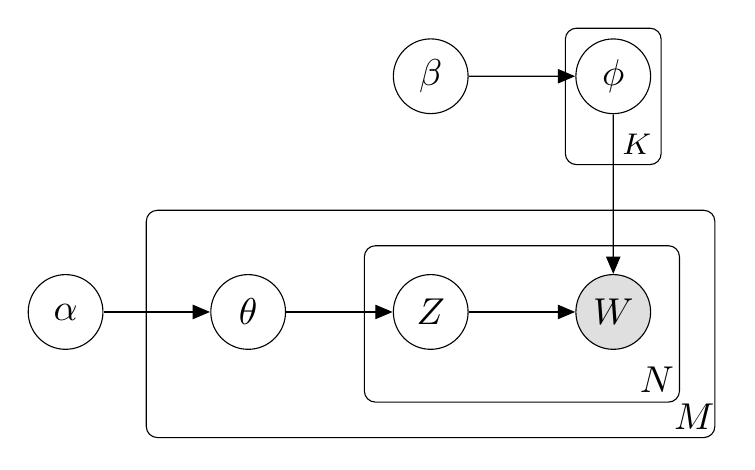
\begin{tikzpicture}[scale=1.35, transform shape]
        % Define nodes
        \node[obs]                               (w) {$W$};
        \node[latent, left=of w] (z) {$Z$};
        \node[latent, left=of z] (theta) {$\theta$};
        \node[latent, left=of theta]            (alpha) {$\alpha$};
        \node[latent, above=of w, yshift=0.5cm]            (phi) {$\phi$};
        \node[latent, left=of phi]              (beta) {$\beta$};

        % Connect the nodes
        \edge {z} {w} ;
        \edge {theta} {z} ;
        \edge {alpha} {theta} ;
        \edge {beta} {phi} ;
        \edge {phi} {w} ;

        % Plates
        \plate [inner sep=0.8cm] {plate1} {(theta)(z)(w)} {} ;
        \plate [inner sep=0.35cm] {plate2} {(w)(z)} {} ;
        \plate {plate3} {(phi)} {$K$} ;

        % Manually adjust label positions
        \node [xshift=-0.2cm, yshift=0.2cm] at (plate1.south east) {$M$};
        \node [xshift=-0.55cm, yshift=0.55cm] at (plate1.south east) {$N$};

    \end{tikzpicture}
    \caption{LDA plate notation}
    \label{fig:lda}
\end{figure}

The generative process for a corpus in the context of LDA is as follows:

\begin{enumerate}
    \item For each document $i = 1, \ldots, M$:
          \begin{itemize}
              \item Sample $\theta$ from a Dirichlet distribution $\theta_i \sim \text{Dir}(\alpha)$.
          \end{itemize}
    \item For each topic $k = 1, \ldots, K$:
          \begin{itemize}
              \item Sample $\phi$ from another Dirichlet distribution $\phi_k \sim \text{Dir}(\beta)$.
          \end{itemize}
    \item For each word $j = 1, \ldots, N$ in document $i$:
          \begin{itemize}
              \item Sample a topic $z_{ij} \sim \text{Multinomial}(\theta_i)$.
              \item Sample a word $w_{ij} \sim \text{Multinomial}(\phi_{z_{ij}})$.
          \end{itemize}
\end{enumerate}

$\theta_{ik}$ represents the probability of the $i$-th document to contain words from the $k$-th topic. Similarly, $\phi_{kw}$ represents the probability of the $k$-th topic to contain the $w$-th word.

\subsection{Dirichlet distribution}

Take the example of a large digital library of academic papers. First, for each paper $i$, we sample its topic distribution $\theta_i$ from a Dirichlet distribution. This represents the mixture of topics covered by the document. Secondly, for each topic $k$, we sample a word distribution $\phi_k$ over each topic from a Dirichlet distribution. Then, for each word $j$ in the document, we draw a topic $z_{ij}$ from the topic distribution Multinomial($\theta_i$), followed by sampling a word $w_{ij}$ from the word distribution Multinomial($\phi_{z_{ij}}$). This process models the generation of words in an academic paper based on latent topic structures and their corresponding word distributions.

The intuition behind the Dirichlet distribution is that the $k$-dimensional Dirichlet distribution $\theta$ is controlled by a $k$-dimensional vector of positive real numbers, $\alpha$. The $\alpha$ parameter shapes how topics are distributed across documents. A uniform $\alpha$ suggests no prior preference for topic prevalence, leading to a balanced mix of topics within documents. Smaller $\alpha$ values push the model towards sparser topic representations, where documents are likely to be dominated by fewer topics. An asymmetric $\alpha$ allows for the modeling of prior beliefs about topic prevalence, making some topics more prominent than others.

Similarly, $\beta$ controls the concentration of the word distribution for each topic, where the $m$-dimensional Dirichlet distribution $\phi$ is controlled by a $m$-dimensional vector of positive real numbers, $\beta$.

\subsection{Learning LDA}

The problem of learning an LDA model is referred to as an "inference" problem. That is, given the observed variable, \( w \), and the hyper-parameters \( \alpha \) and \( \beta \), how do we estimate the posterior of the latent variables:

\[ p(\theta, z, \phi | w, \alpha, \beta) = \frac{p(\theta, z, \phi, w | \alpha, \beta)}{p(w | \alpha, \beta)} \]

\citet{blei_latent_2001} discover that the integral for computing in the denominator is infeasible to compute exactly:

\[ p(w | \alpha, \beta) = \frac{\Gamma(\sum_i \alpha_i)}{\prod_i \Gamma(\alpha_i)} \int \left( \prod_i \theta_i^{\alpha_i - 1} \right) \left( \prod_{n=1}^{N} \prod_{i=1}^{k} \prod_{j=1}^{V} (\theta_i \beta_{ij})^{w_{n}} \right) d\theta \]

Therefore, approximate inference must be applied. Common approaches are Gibbs sampling and variational inference. Without delving into too much detail, Gibbs sampling allows us to avoid directly computing the intractable integral. The basic idea is that we want to sample from \(p(w \mid \alpha, \beta)\) to estimate the distribution, but we cannot directly do so. Instead, Gibbs sampling allows us to iteratively compute the posterior of one of the latent variables while fixing all the other variables. This way, we can obtain the posterior distribution \(p(\theta, z, \phi \mid w, \alpha, \beta)\).

For each iteration, we alternatively sample \(\theta\), \(z\), \(\phi\) with all the other variables fixed. Because the samples from the early iterations are not stable, we discard the first \(B\) iterations of samples. The algorithm is shown in the following pseudo code:


For \(i\) from \(1\) to \(\text{MaxIter}\):
\begin{itemize}
    \item Sample \(\theta_{i} \sim p(\theta \mid z = z_{i-1}, \phi = \phi_{i-1}, w, \alpha, \beta)\)
    \item Sample \(z_{i} \sim p(z \mid \theta = \theta_{i}, \phi = \phi_{i-1}, w, \alpha, \beta)\)
    \item Sample \(\phi_{i} \sim p(\phi \mid \theta = \theta_{i}, z = z_{i}, w, \alpha, \beta)\)
\end{itemize}

The algorithm begins with initial, possibly random, values for the variables \(\theta\), \(z\), and \(\phi\), and proceeds through a series of iterations up to a predefined maximum number, \(\text{MaxIter}\). At each iteration \(i\), the value of \(\theta_i\) is sampled from its conditional distribution given the current values of \(z\) and \(\phi\), denoted \(z_{i-1}\) and \(\phi_{i-1}\) to reflect their values from the previous iteration, alongside any observed data or parameters \(w\), \(\alpha\), and \(\beta\). Following this, \(z_i\) is updated based on the new \(\theta_i\) and the previous \(\phi_{i-1}\), and finally, \(\phi_i\) is sampled using the latest values of \(\theta_i\) and \(z_i\). This sequential updating of variables leverages the simpler conditional distributions to approximate the complex joint distribution. As the number of iterations increases, the algorithm converges, meaning the samples generated become representative of the target distribution.

\section{Non-negative Matrix Factorization}
Non-negative Matrix Factorization (NMF) \cite{shahnaz_document_2006, kasiviswanathan_emerging_2011, yan_learning_2013} is a technique where an original matrix, consisting of non-negative values, is decomposed into two distinct matrices. The fundamental principle of NMF is that the product of these two matrices approximates the original matrix. This decomposition is a form of dimensionality reduction. The large original matrix typically represents a set of documents, with each document being a vector of words. The two resultant matrices in NMF are the word-topic matrix and the topic-document matrix. The topic-word matrix shows the association between topics and words, while the topic-document matrix shows the relationship between topics and individual documents.

\Cref{fig:nmf} illustrates the decomposition of a matrix \(A\) into two matrices \(W\) and \(H\). The matrix \(A\) is a non-negative matrix, and the matrices \(W\) and \(H\) are also non-negative. The product of \(W\) and \(H\) approximates \(A\). \(A\) represents the word-document matrix, where each row corresponds to a word and each column corresponds to a document. \(W\) represents the word-topic matrix, where each row corresponds to a word and each column corresponds to a topic. \(H\) represents the topic-document matrix, where each row corresponds to a topic and each column corresponds to a document.

\begin{figure}[h] % adjust placement if needed
    \centering
    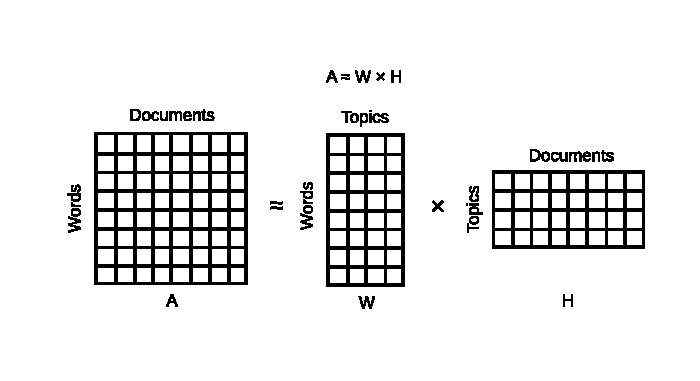
\includegraphics[width=0.75\textwidth]{figures/nmf.pdf}
    \caption{NMF decomposition}
    \label{fig:nmf}
\end{figure}

Non-negative Matrix Factorization is a group of algorithms whose objective is to minimize $F$ - the function which measures the error between the original matrix and the product of the two matrices. The most common algorithms for NMF typically involve iterative update rules that aim to minimize $F$, such as the Frobenius norm or the Kullback-Leibler (KL) divergence.

\subsection{Frobenius norm}

The goal in NMF using the Frobenius norm is to minimize the objective function \( F \), which is given by:

\[
    F = \| A - WH \|_F^2 = \sum_{i=1}^{n} \sum_{j=1}^{m} (A_{ij} - (WH)_{ij})^2
\]

where \( \| \cdot \|_F \) denotes the Frobenius norm. This objective function represents the sum of the squares of the element-wise differences between \( A \) and the product \( WH \).

The typical algorithm to minimize the Frobenius norm in NMF is an iterative process that involves:

\begin{enumerate}
    \item \textbf{Initialization:} Matrices \( W \) and \( H \) are initialized with non-negative values. This can be done randomly or based on some informed heuristic.
    \item \textbf{Iterative Update:} The matrices \( W \) and \( H \) are updated iteratively to reduce \( F \). The updates are performed using multiplicative rules that inherently maintain the non-negativity of \( W \) and \( H \). The update rules are as follows:
          \[
              W_{ai} \leftarrow W_{ai} \cdot \frac{(AH^\top)_{ai}}{(WHH^\top)_{ai}}
          \]
          \[
              H_{ib} \leftarrow H_{ib} \cdot \frac{(W^\top A)_{ib}}{(W^\top WH)_{ib}}
          \]
          where the indices \( a \) and \( b \) iterate over all rows and columns of \( W \) and \( H \), respectively.
    \item \textbf{Convergence:} The iteration continues until the change in \( F \) between successive iterations is less than a predetermined threshold, or a maximum number of iterations has been reached.
\end{enumerate}

While the Frobenius norm-based NMF is not convex over both \( W \) and \( H \) together, it is convex over each one individually when the other is held constant. Thus, each iteration is guaranteed to not increase \( F \), although the solution may converge to a local minimum rather than a global minimum.

\subsection{Kullback-Leibler}

Unlike the Frobenius norm which assesses the difference based on squared errors, the KL divergence is more suitable for data that is inherently probabilistic. The KL divergence for two matrices is defined as:

\[
    D(A || WH) = \sum_{i=1}^{n} \sum_{j=1}^{m} \left( A_{ij} \log\frac{A_{ij}}{(WH)_{ij}} - A_{ij} + (WH)_{ij} \right)
\]

where \( D(A || WH) \) represents the KL divergence between \( A \) and \( WH \), with the objective to minimize this divergence in NMF.

The iterative update rules for the matrices \( W \) and \( H \) that minimize the KL divergence are as follows:

\[
    W_{ai} \leftarrow W_{ai} \cdot \frac{(A \oslash (WH)H^\top)_{ai}}{\mathbf{1}H^\top_{ai}}
\]

\[
    H_{ib} \leftarrow H_{ib} \cdot \frac{(W^\top(A \oslash (WH)))_{ib}}{W^\top\mathbf{1}_{ib}}
\]

Here, \( \oslash \) denotes element-wise division, and \( \mathbf{1} \) is a matrix of ones that is used for normalization in the denominators.

Just like in the case of the Frobenius norm, the KL divergence-based NMF aims to iteratively update \( W \) and \( H \) until the decrease in \( D(A || WH) \) is below a certain threshold, signaling convergence. However, it is important to note that this optimization problem is non-convex, and the solution found may represent a local minimum.

\section{Top2Vec}
A limitation of LDA and NMF is that they disregard semantic relationships between words, thus neglecting context. As a result, text embedding techniques which capture context have become popular as an NLP technique.

\subsection{Embeddings}

In Top2Vec \cite{angelov_top2vec_2020}, the first step is to embed the documents into dense vector representations (embeddings) to capture the semantic meaning of the text. \Cref{fig:doc_word_embedding} \cite{angelov_top2vec_2020} illustrates the embeddings, where the purple dots represent words and the green dots represent documents. Words are closest to documents that contain them, and documents are closest to words that are most representative of their content.

\begin{figure}[h] % adjust placement if needed
    \centering
    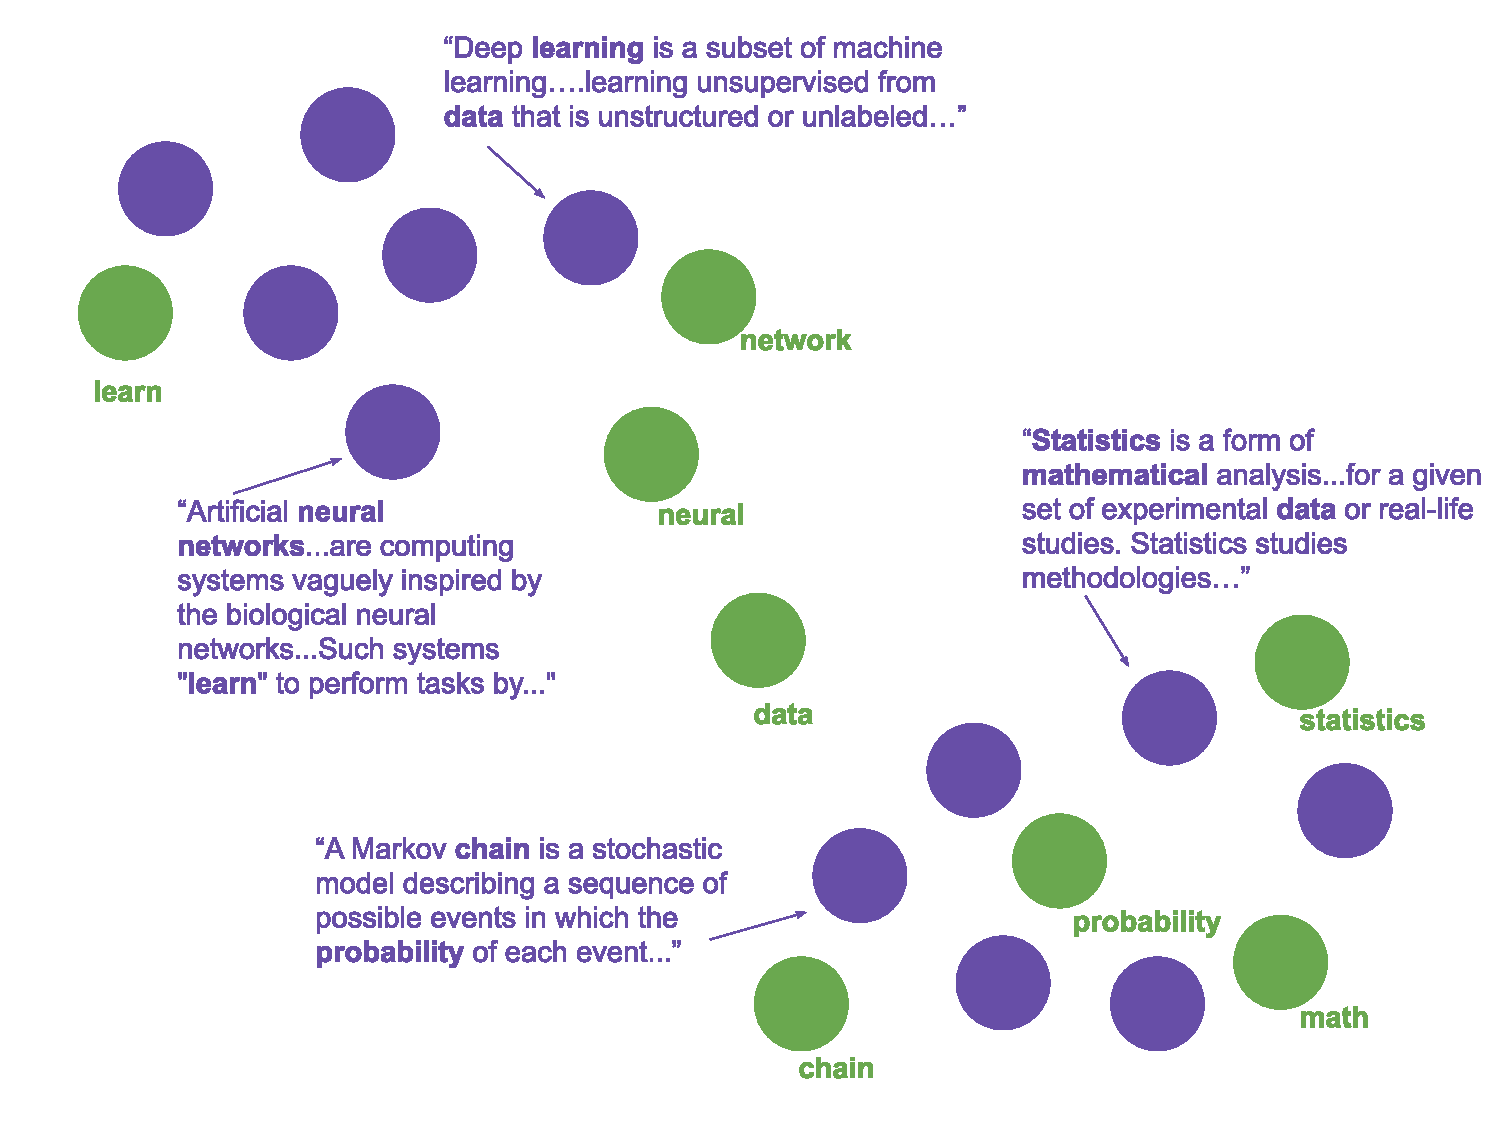
\includegraphics[width=0.65\textwidth]{figures/doc_word_embedding.pdf}
    \caption{Example of embeddings}
    \label{fig:doc_word_embedding}
\end{figure}

To learn the embeddings, Top2Vec utilizes Doc2Vec \cite{le_distributed_2014, rehurek_software_2010}, Universal Sentence Encoder \cite{cer_universal_2018}, or Sentence-BERT (SBERT) \cite{reimers_sentence-bert_2019}.

The original paper uses Doc2Vec's Distributed Bag of Words (DBOW) model, and even though it is simpler than Doc2Vec's Distributed Memory (DM) model, it is more efficient and has been shown to perform better in practice \cite{lau_empirical_2016}. DBOW essentially uses the document vector to predict words within a context window in the document.

Doc2Vec's DBOW is similar to Word2Vec's Skip-gram model (\cref{sec:word_embedding_topic_models}), which uses the context word to predict surrounding words in the context window. The difference is that DBOW switches the context word for the document vector to predict the surrounding words in the context window.

The process of learning the embeddings in Top2Vec can be summarized as follows:
\begin{enumerate}
    \item \textbf{Matrix Initialization}: The process initiates with the establishment of two matrices. The document matrix, denoted as $D_{c,d}$, encapsulates document vectors where $c$ represents the corpus's document count and $d$ the embedding dimensionality. Each row within $D_{c,d}$ represents a distinct document vector $\vec{d} \in \mathbb{R}^d$. Concurrently, the context word matrix $W'_{n,d}$, representing word vectors in analogous $d$-dimensional space for $n$ vocabulary words, may originate from pre-training, random initialization, or parallel learning processes.

    \item \textbf{Word Prediction Mechanism}: Contrary to relying on neighboring context words for prediction, the DBOW model employs the document vector for prediction. For every document $d$, each word's context vector $\vec{w_c}'$ within $d$ (sourced from $W'_{n,d}$) aids in inferring the document's vector $\vec{d}$ in $D_{c,d}$. This inference employs a softmax function, $\text{softmax}(\vec{w_c}' \cdot D_{c,d})$, generating a corpus-wide probability distribution reflecting each document's likelihood of generating the word.

    \item \textbf{Learning Process}: The learning process aims to optimize the document and word vectors to predict the document's constituent words. This optimization leverages backpropagation and stochastic gradient descent to modify both $D_{c,d}$ and $\vec{w_c}'$ from $W'_{n,d}$ to maximize the probability $P(\vec{d} | \vec{w})$ of correctly predicting the document given its words.

    \item \textbf{Embeddings}: Through optimization, embeddings emerge where documents gravitate towards the vectors of words they comprise, effectively "attracted" by these words. Consequently, semantically similar documents (sharing similar words) cluster, whereas dissimilar documents (sharing fewer words) diverge.
\end{enumerate}

\subsection{Number of topics}

In the embeddings, a dense area of documents can be interpreted as an area of highly similar documents. First, Uniform Manifold Approximation and Projection for Dimension Reduction (UMAP) \cite{mcinnes_umap_2020} is used to reduce the dimensionality of the document vectors. That is because the high-dimensional document vectors lead to the \textit{curse of dimensionality}, where the document vector sparsity makes it difficult to find dense clusters. Then, in order find the dense areas of documents in the embeddings, density-based clustering is used on the document vectors, specifically Hierarchical Density-Based Spatial Clustering of Applications with Noise (HDBSCAN) \cite{campello_density-based_2013, mcinnes_accelerated_2017, mcinnes_hdbscan_2017}. HDBSCAN assigns a label to each dense cluster of document vectors and assigns a noise label to all document vectors that are not in a dense cluster.


\subsection{Topic vectors}

Given labels for each cluster of dense documents in the embeddings, topic vectors can be calculated. The authors lay out multiple methods for calculating topic vectors, but discover that they perform similarly. The method that is used in the original paper is to calculate the centroid of the document vectors in each cluster. The centroid is the average of all the document vectors in the cluster. The centroid is calculated for each set of document vectors that belong do a dense cluster, generating a topic vector for each set. The number of dense areas found is the number of prominent topics identified in the corpus.

In the embeddings, every point represents a topic that is best described semantically by its nearest word vectors. Therefore, the word vectors that are closest to a topic vector are those that are most representative of it semantically. The distance of each word vector to the topic vector will indicate how semantically similar the word is to the topic. The words closest to the topic vector can be seen as the words that are most similar to all documents into the dense area, as the topic vector is the centroid of that area. These words can be used to summarize the common topic of the documents in the dense area.

\section{BERTopic}
Top2Vec simplifies the process of generating topics by clustering embeddings of words and documents. Inspired from Top2Vec, BERTopic \cite{grootendorst_bertopic_2022} is a state-of-the-art topic model that builds on top of the embeddings approach.

BERTopic generates representations of topics through a six-step process:

\begin{enumerate}
    \item Initially, it transforms each document into an embedding using a pre-trained language model.
    \item Before the clustering process, the dimensionality of these embeddings is reduced.
    \item Following this, the embeddings are clustered.
    \item Subsequently, a bag-of-words representation is generated for each cluster, containing the frequency of every word.
    \item Next, topic representations are derived from these clusters using a specialized class-based version of TF-IDF.
    \item The final step optionally fine-tunes these topic representations. Each of these steps is modular, allowing for the use of different techniques at each stage.
\end{enumerate}

While these steps are the default, BERTopic offers a degree of modularity. Each step in the process is relatively independent from the others. For instance, the bag-of-words step does not depend on the specific embedding model used for document embeddings, which provides flexibility in how the bag-of-words representation is calculated.

As a result, BERTopic is highly modular, maintaining its ability to generate topics across different sub-models. This means that BERTopic effectively allows for the construction of customized topic models, appropriate for the specific use case. Additionally, the modularity of BERTopic ensures that it can be easily adapted to incorporate new advancements in the field of NLP, since each component can be changed independently from the others. \Cref{fig:modularity_modified} (inspired by \cite{grootendorst_algorithm_nodate}) illustrates the six steps of BERTopic, presented from bottom to top. It highlights the possibility of employing various techniques at each step of the process. For example, one could choose between SBERT or spaCy for document embedding, UMAP \cite{mcinnes_umap_2020} or PCA \cite{abdi_principal_2010} for dimensionality reduction, and GPT or KeyBERT \cite{grootendorst_maartengrkeybert_2024} for the fine-tuning phase.

\begin{figure}[h] % adjust placement if needed
    \centering
    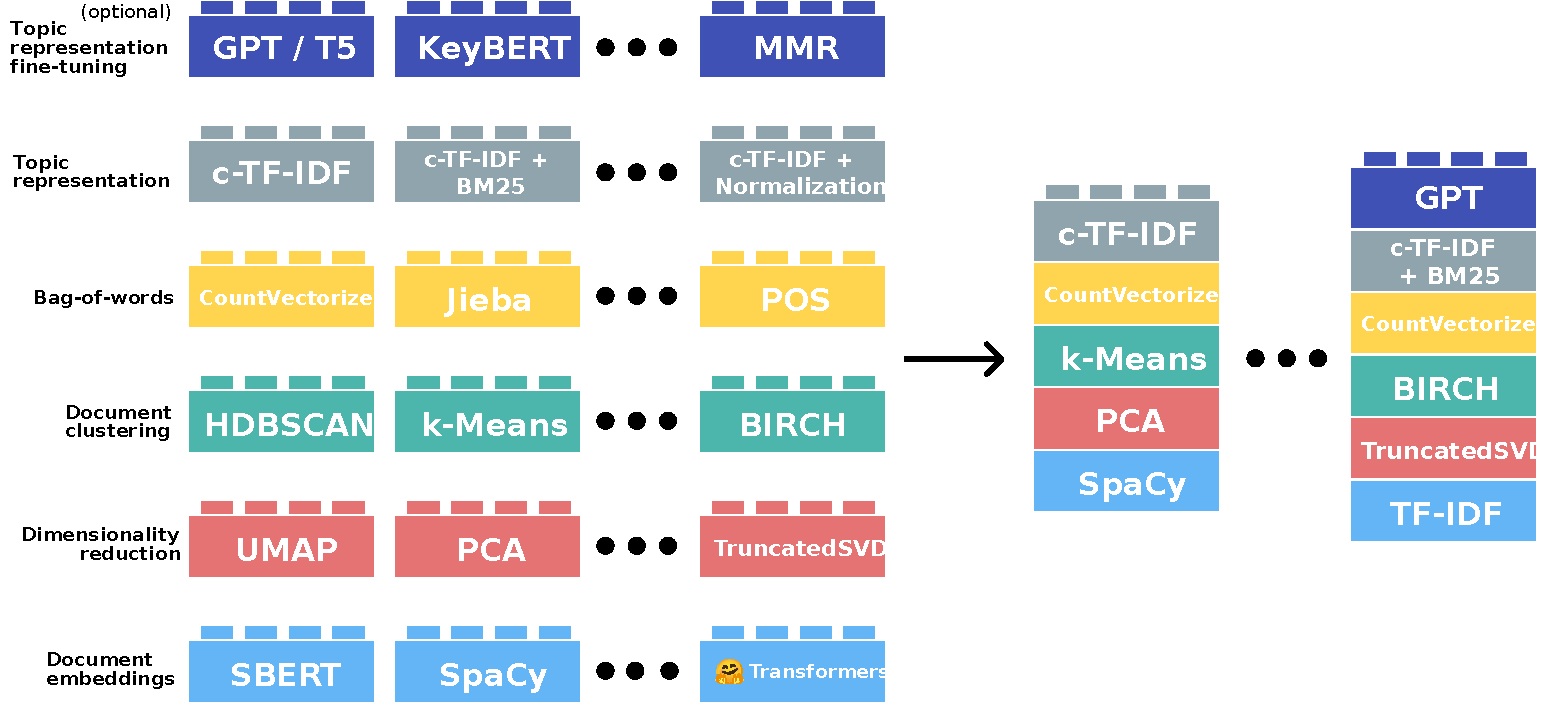
\includegraphics[width=\textwidth]{figures/modularity_modified.pdf}
    \caption{BERTopic modularity and steps (from bottom to top)}
    \label{fig:modularity_modified}
\end{figure}

\subsection{Document embeddings}

In BERTopic, documents are transformed into embeddings to create vector space representations for semantic comparison. It is based on the idea that documents sharing the same topic will have similar semantics. For this embedding step, by default BERTopic utilizes the SBERT framework \cite{reimers_sentence-bert_2019}. SBERT is a modification of the popular Bidirectional Encoder Representations from Transformer (BERT) model (\cref{sec:transformer_based_models}), and enables the conversion of sentences and paragraphs into dense vector representations by employing pre-trained language models. This achieves top performance on several sentence embedding tasks \cite{reimers_making_2020}. The embeddings are mainly used for clustering documents with semantic similarities rather than directly for topic generation.

The base Transformer architecture is presented in \cref{fig:transformer} \cite{vaswani_attention_2017}. It uses a unidirectional multi-head self-attention mechanism to capture dependencies between words in a sentence. Unidirectional means that the attention mechanism only looks at previous words in the sentence, which can be a limitation. The model consists of a stacked encoder-decoder architecture, where the encoder processes the input sequence, and the decoder generates the output sequence. The encoder is composed of a stack of identical layers, each containing two sub-layers: a multi-head self-attention mechanism and a feed-forward neural network. The decoder is also composed of a stack of identical layers, each containing three sub-layers: a multi-head self-attention mechanism, a multi-head attention mechanism over the encoder's output, and a feed-forward neural network. The self-attention mechanism allows the model to weigh the importance of each word in the sentence when generating the embeddings.

\begin{figure}[h]
    \centering
    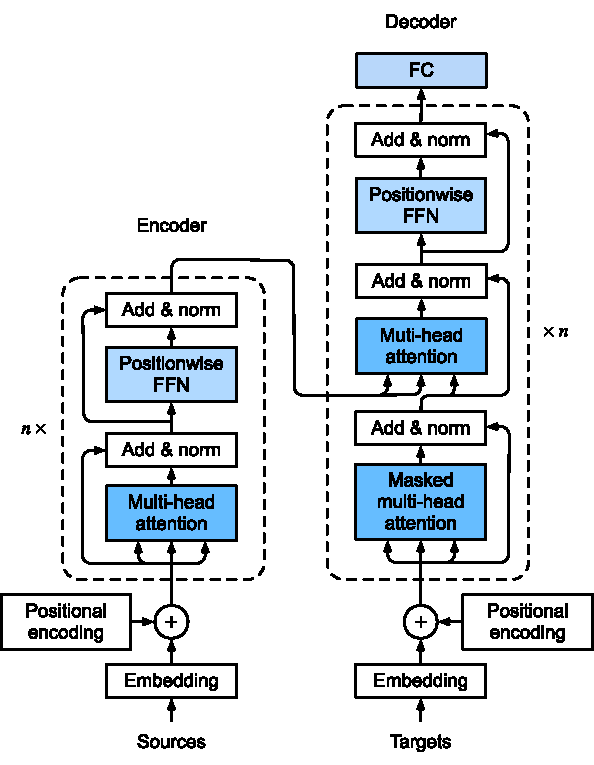
\includegraphics[width=0.5\textwidth]{figures/transformer.pdf}
    \caption{Transformer architecture}
    \label{fig:transformer}
\end{figure}

BERT, in contrast, is a bidirectional model that captures dependencies between words in both directions (\cref{fig:bert}, \cref{fig:gpt}, \cref{fig:bert_detailed}) \cite{vaswani_attention_2017, devlin_bert_2019}. It achieves this by leveraging a \textit{masked language model (MLM)} objective, where the model is trained to predict masked words within a sentence. Pre-trained on a large corpus of text, BERT’s embeddings can be fine-tuned for various downstream tasks, such as sentence classification or question answering. However, tasks relevant to topic modeling, such as semantic similarity, are computationally expensive due to BERT's cross-encoder architecture. In a cross-encoder, pairs of sentences are passed through the transformer network together, and the target value is predicted. For example, in a collection of \( n = 10,000 \) sentences, finding the most similar pair using BERT would require \( n \times (n-1) / 2 = 49,995,000 \) inference computations \cite{reimers_sentence-bert_2019}.

\begin{figure}[h]
    \centering
    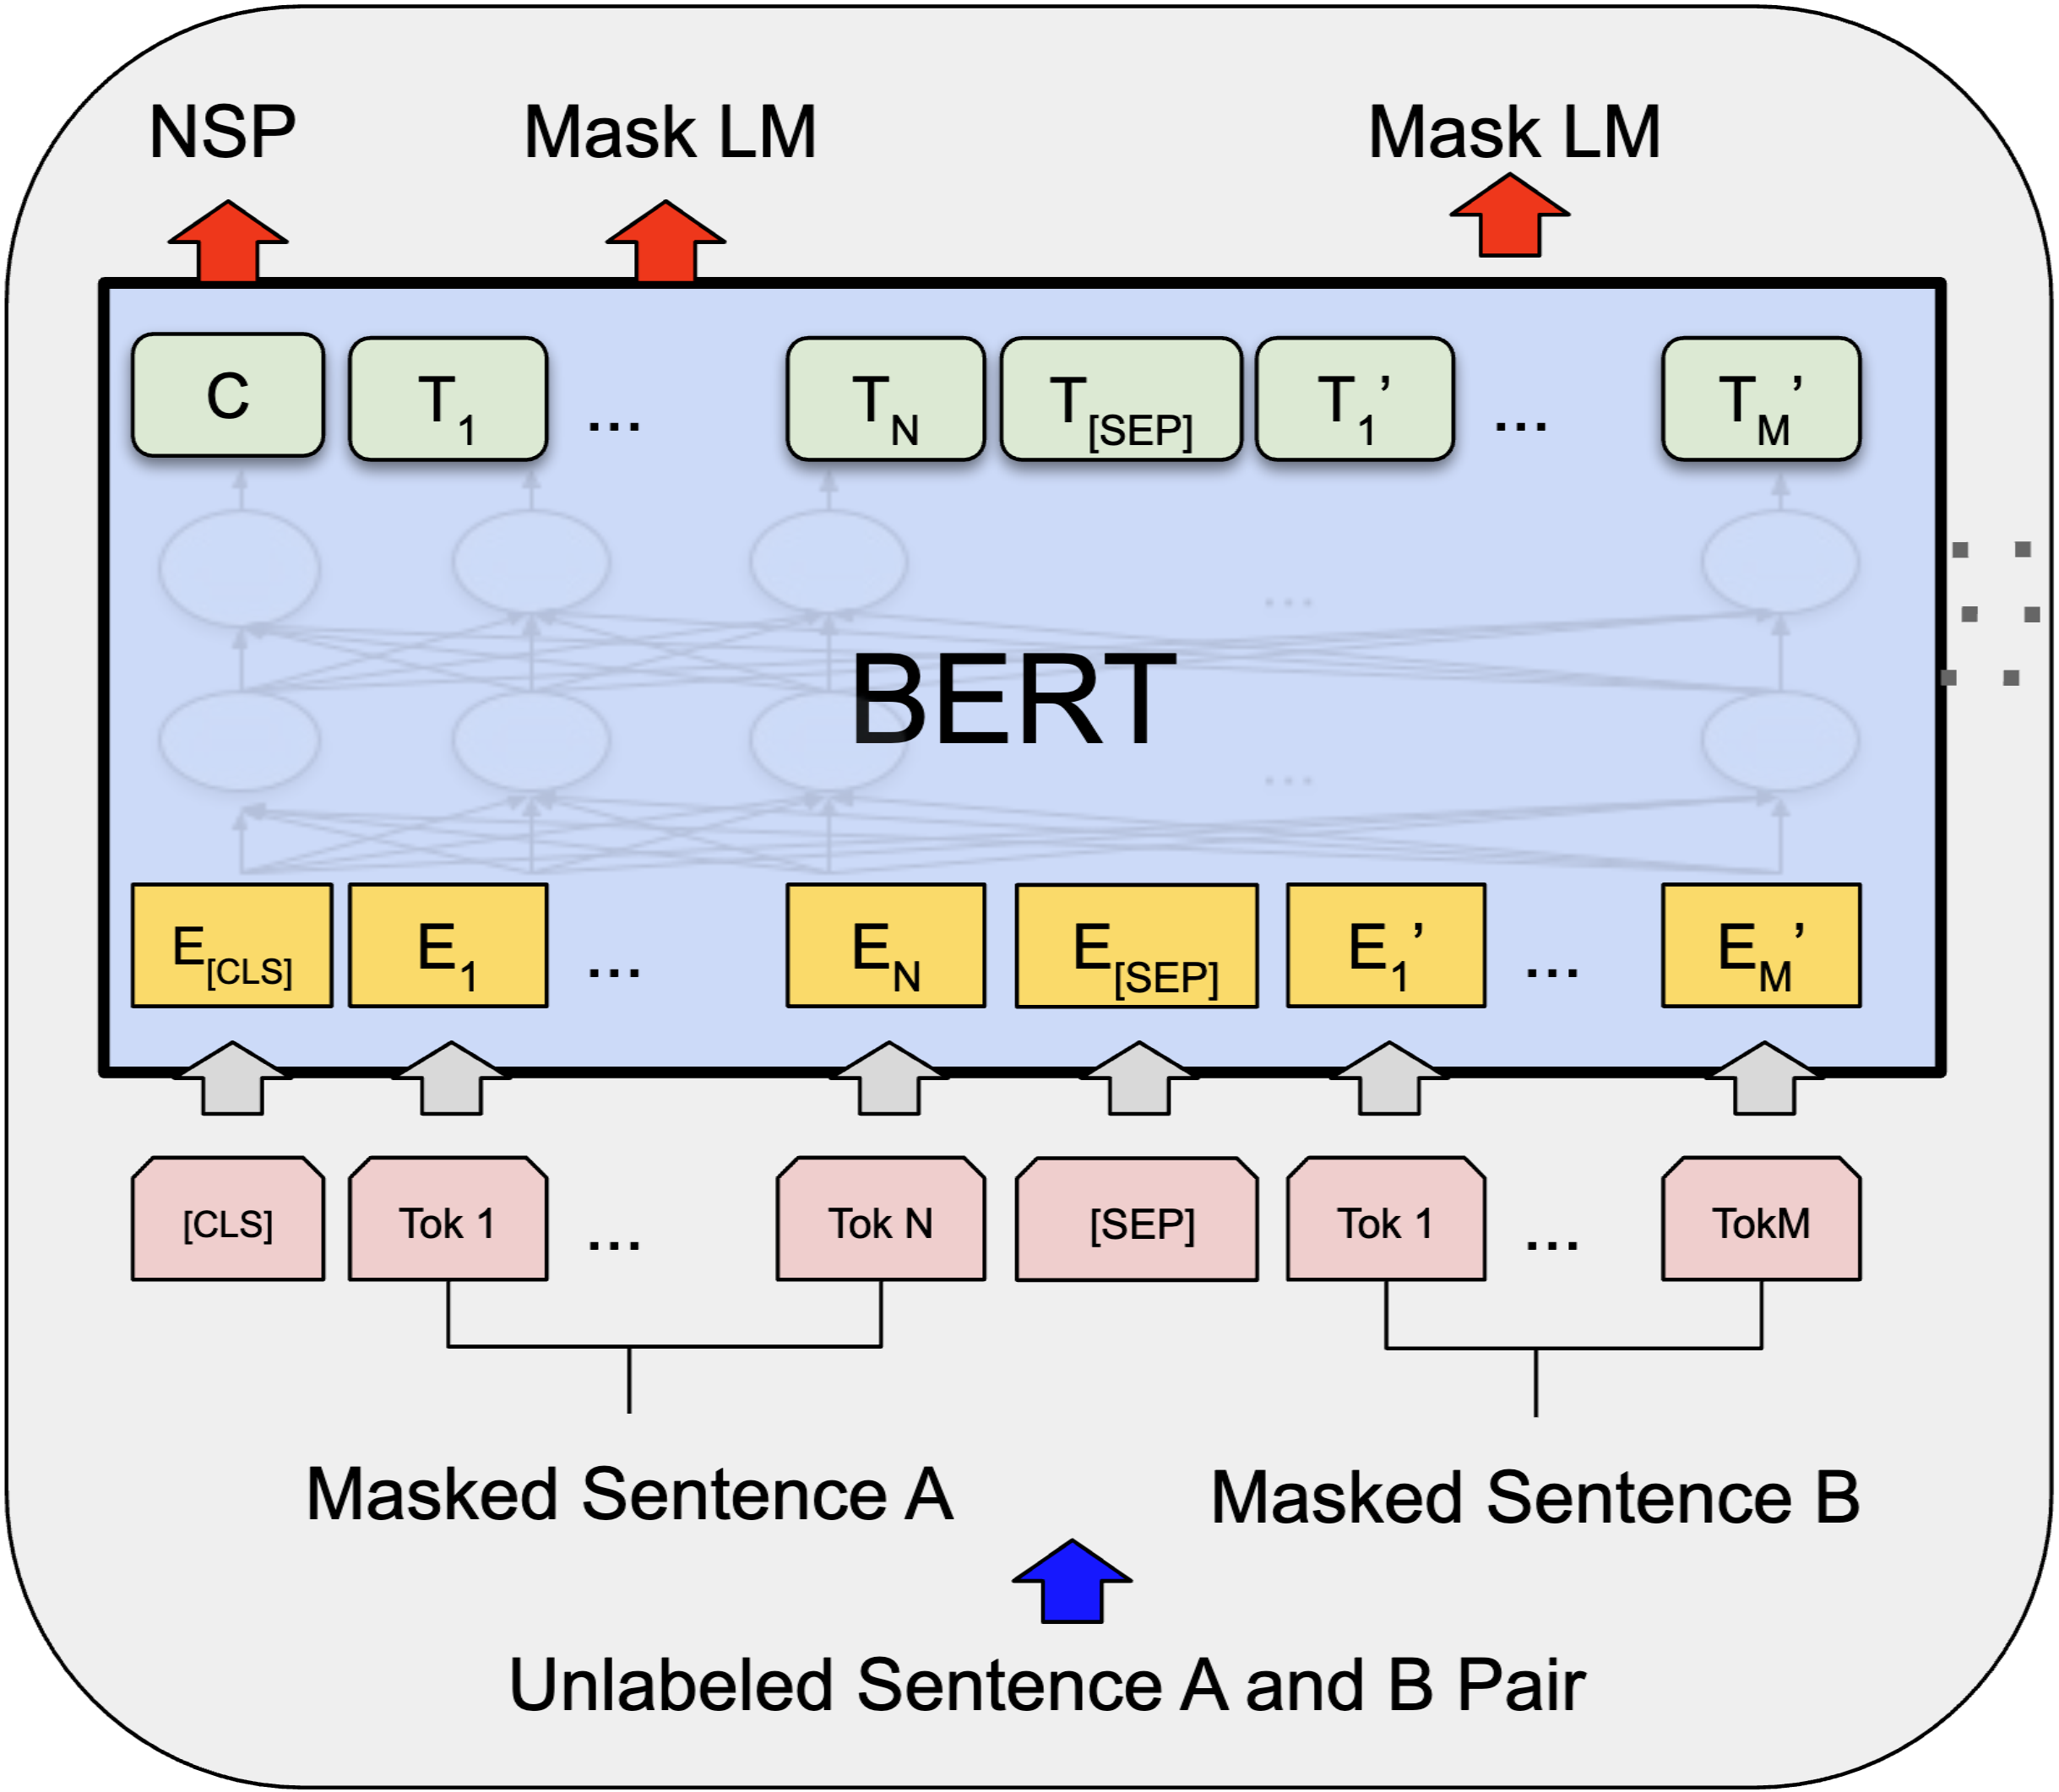
\includegraphics[width=0.5\textwidth]{figures/bert_detailed.png}
    \caption{Transformer architecture}
    \label{fig:bert_detailed}
\end{figure}

\begin{figure}[h]
    \centering
    \begin{minipage}[b]{0.40\textwidth}
        \centering
        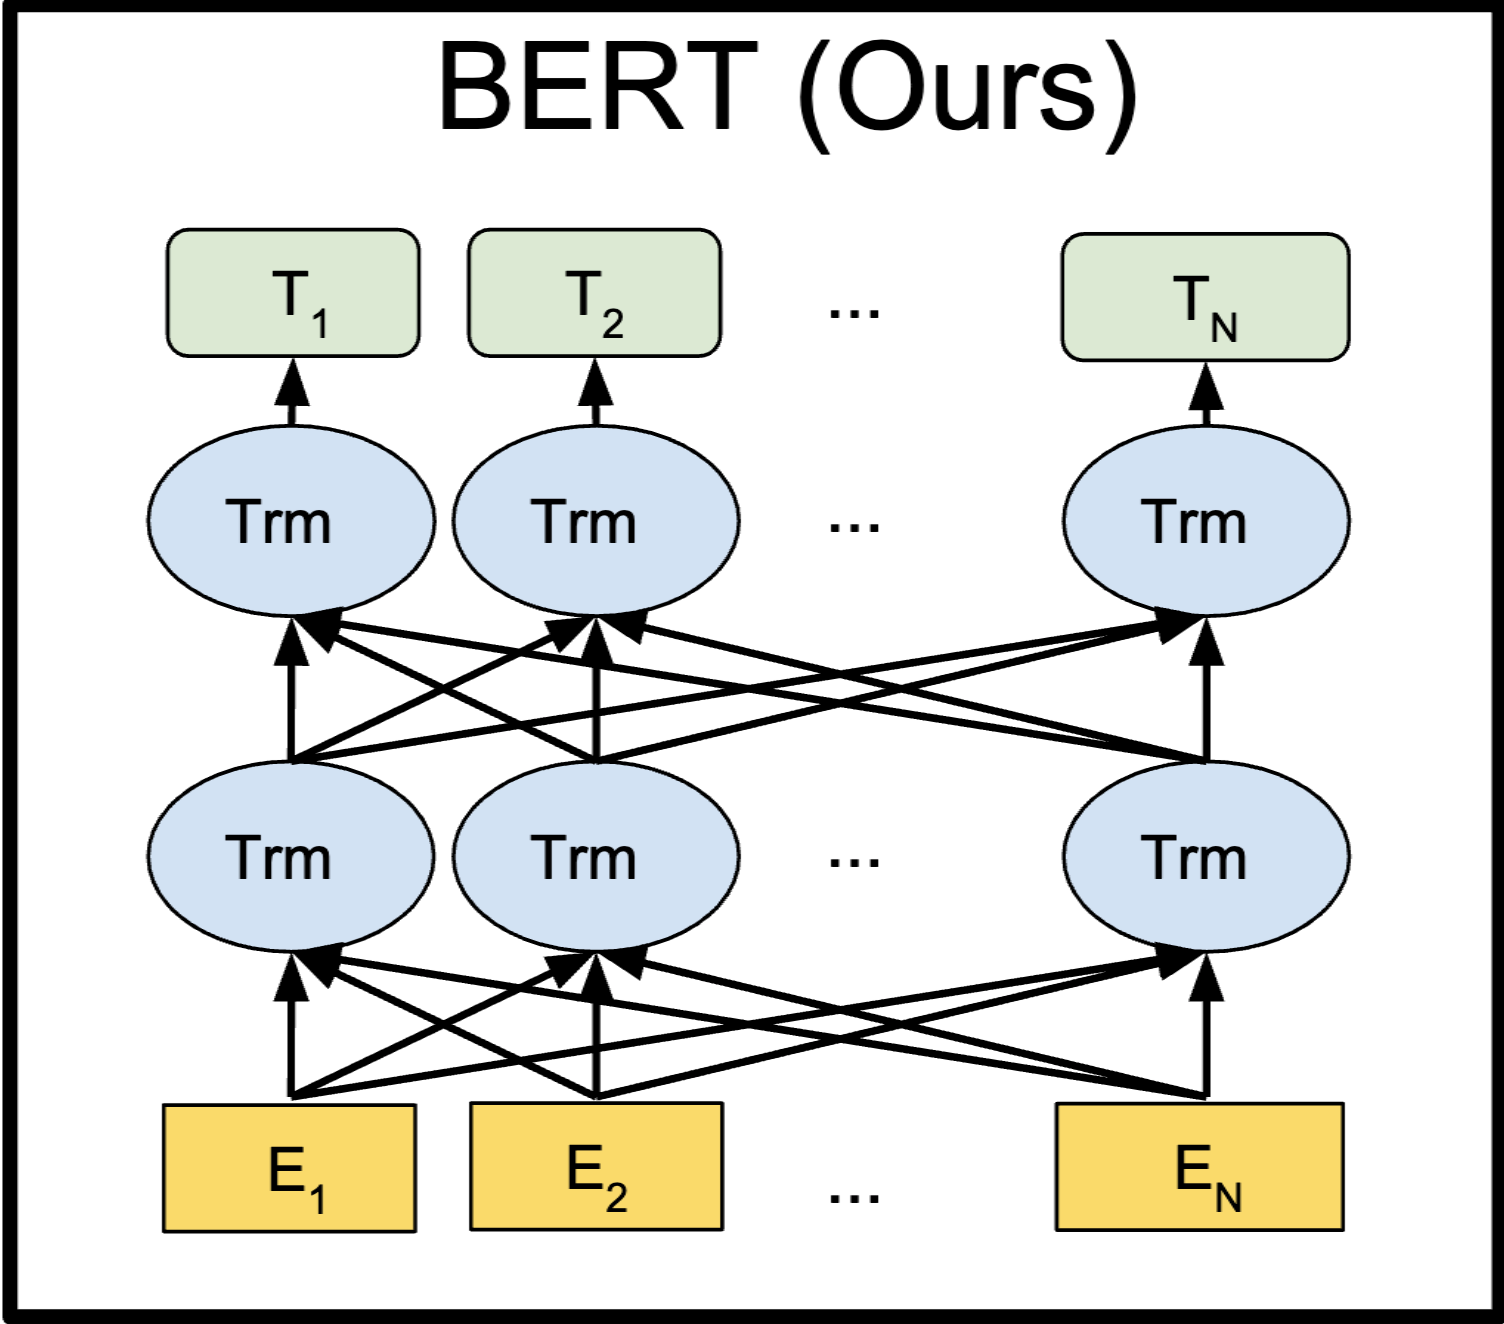
\includegraphics[width=\textwidth]{figures/bert.png}
        \caption{BERT Bidirectional Architecture}
        \label{fig:bert}
    \end{minipage}
    \hfill
    \begin{minipage}[b]{0.39\textwidth}
        \centering
        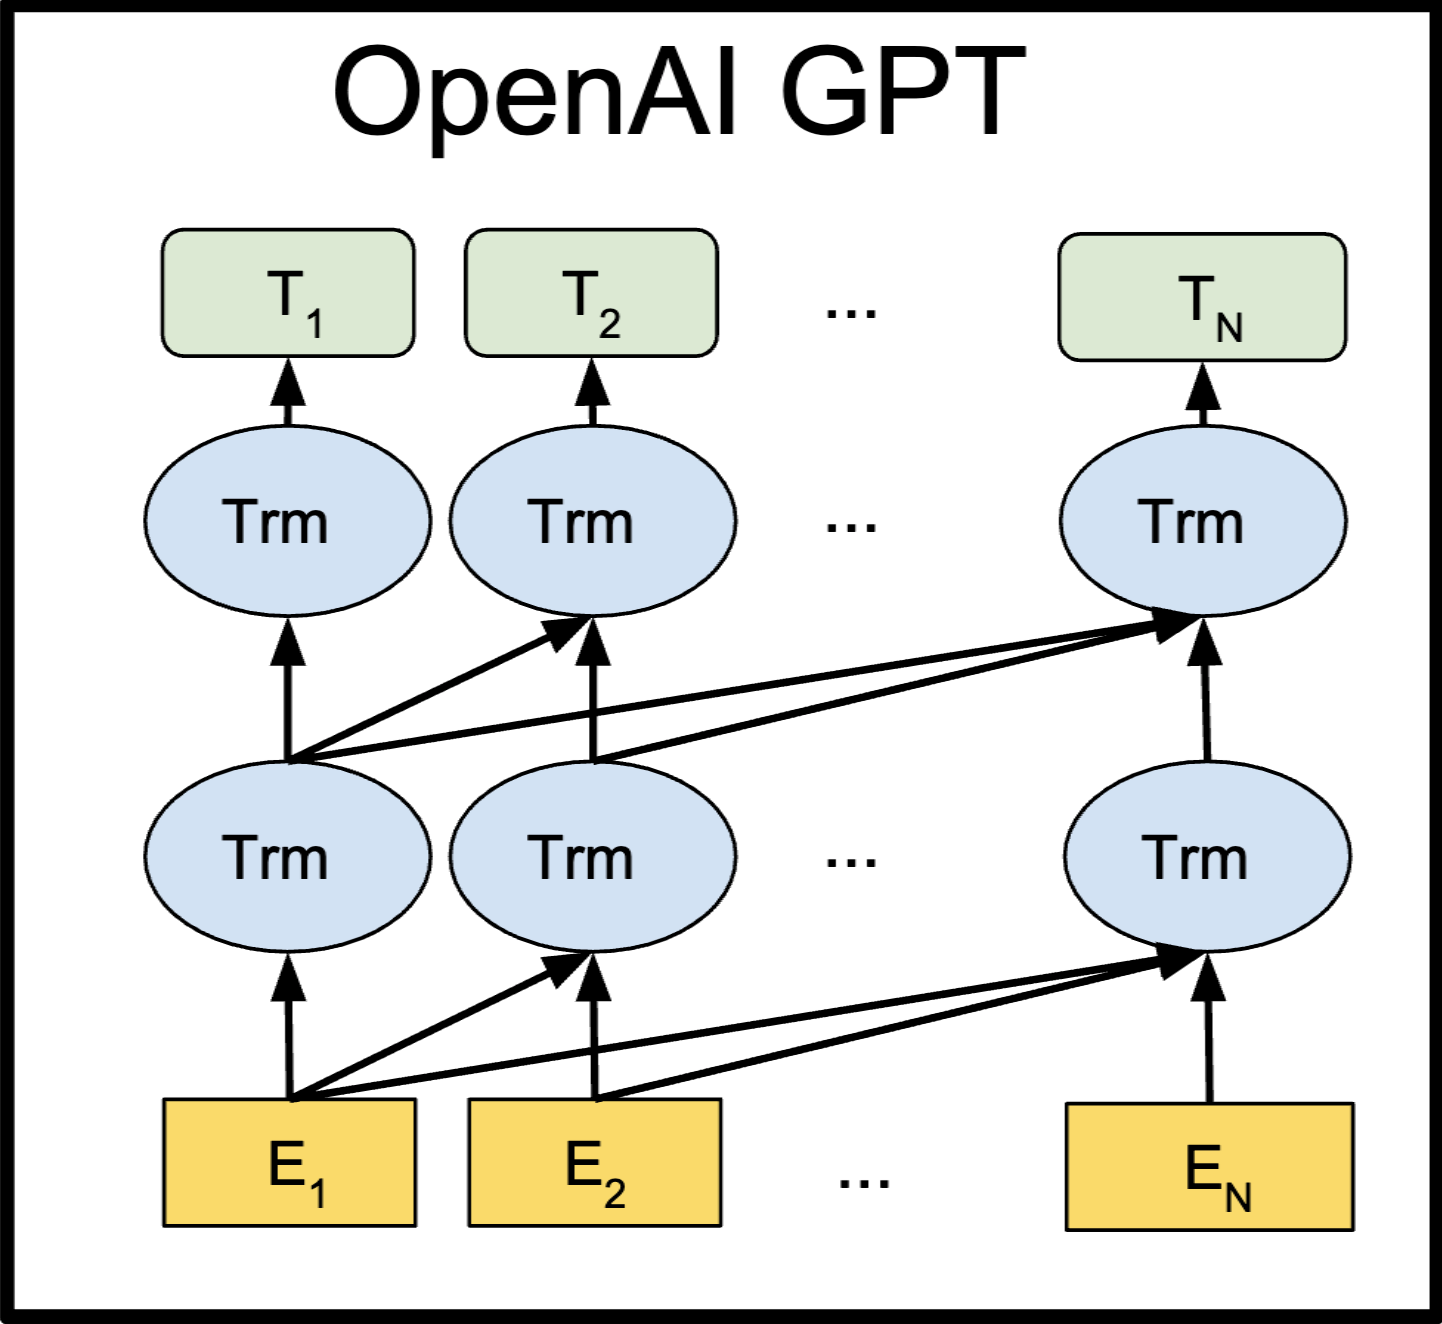
\includegraphics[width=\textwidth]{figures/openai.png}
        \caption{OpenAI GPT Unidirectional Architecture}
        \label{fig:gpt}
    \end{minipage}
\end{figure}

SBERT addresses this issue by incorporating a Siamese network architecture with a bi-encoder setup, where two identical BERT models share the same weights (\cref{fig:bi_vs_cross}). In SBERT, each sentence is processed independently, and the embeddings are computed separately. As a result, for \( n = 10,000 \) sentences, only 10,000 inference computations are needed. Once the embeddings are generated, similarity can be easily calculated, as it is a computationally efficient operation.

\begin{figure}[h]
    \centering
    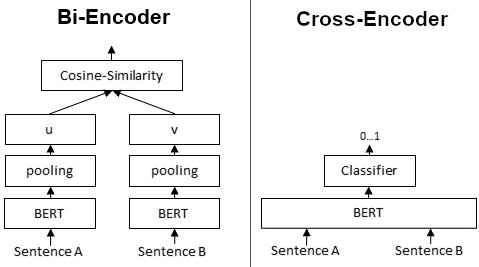
\includegraphics[width=0.6\textwidth]{figures/bi_vs_cross.png}
    \caption{Transformer architecture}
    \label{fig:bi_vs_cross}
\end{figure}

BERTopic can use any embedding technique or architecture, provided the language model used for generating document embeddings is fine-tuned for semantic similarity. Hence, the quality of BERTopic's clustering improves as more advanced language models are developed, allowing BERTopic to evolve alongside advancements in embedding techniques. This proves particularly useful in the context of topic modeling, since the quality of the embeddings directly influences the quality of the topics generated.

The Massive Text Embedding Benchmark (MTEB) \cite{muennighoff_mteb_2023} is a benchmark that evaluates the performance of various embedding models on a wide range of tasks. It provides a comprehensive comparison of the performance of different embedding models, including SBERT, RoBERTa \cite{liu_roberta_2019}, and BERT. By leveraging MTEB, the user can select the most suitable embedding model for their specific use case.

\subsection{Dimensionality reduction}

As the dimensionality of data (embeddings) increases, the distance to the nearest data point tends to become similar to the distance to the farthest data point \cite{aggarwal_surprising_2001, beyer_when_1999}. This phenomenon implies that in high-dimensional spaces, the notion of spatial locality becomes unclear, and distances between points become increasingly small. While several clustering methods have been developed to address this \textit{curse of dimensionality} \cite{pandove_systematic_2018, steinbach_challenges_2004}, a simpler strategy involves reducing the dimensionality of embeddings. Although PCA \cite{abdi_principal_2010} and t-SNE \cite{van_der_maaten_visualizing_2008} are popular dimensionality reduction techniques, UMAP has been found to better preserve the local and global characteristics of high-dimensional data in its lower-dimensional representations \cite{mcinnes_umap_2020}.

UMAP is a non-linear dimensionality reduction technique that is rooted in manifold learning and is mathematically grounded in \textit{topological data analysis}. More specifically, UMAP seeks to approximate a high-dimensional manifold by constructing a weighted k-nearest neighbor (k-NN) graph and then optimizing a low-dimensional layout of this graph.

The theory behind UMAP is mathematically complex, but the algorithm can be summarized as follows:

1. \textbf{Constructing the k-NN Graph}:\\
The initial phase of UMAP involves constructing a k-nearest neighbor graph from the high-dimensional data. In this step, for each data point, the algorithm identifies its nearest neighbors based on a distance metric (such as Euclidean distance). The choice of $k$ determines the number of neighbors to consider, and this influences the local structure captured by the graph. Importantly, UMAP assumes that the data points are uniformly distributed on the underlying manifold, and it computes a local distance metric for each point using \textit{Riemannian geometry}. This local metric is based on the distance to the $k$-th nearest neighbor, creating a unique distance function for each point.

2. \textbf{Fuzzy Simplicial Complex Representation}:\\
Once the k-NN graph is built, UMAP constructs a fuzzy simplicial complex. This is a crucial step rooted in \textit{topological data analysis}. Instead of a binary decision about whether or not a point belongs to a neighborhood, UMAP assigns fuzzy membership values to reflect the probability of points being connected. This fuzzy approach smooths out the local connectivity of the manifold. The fuzzy simplicial set is built by combining local fuzzy simplicial sets of each point, using a probabilistic union operation to merge the connections between points. This union operation involves combining the fuzzy memberships of edges (1-simplices) between points, which can be expressed mathematically as $w(e) = a + b - ab$, where $a$ and $b$ are the fuzzy membership probabilities for the edge in each direction, and $w(e)$ is the resulting combined weight.

3. \textbf{Low-Dimensional Embedding Optimization}:\\
After constructing the fuzzy topological representation, UMAP seeks to optimize a low-dimensional embedding that preserves the topological structure of the original data. This process can be viewed as a \textit{graph layout problem}. UMAP minimizes the cross-entropy between the fuzzy topological structures of the high-dimensional data and the low-dimensional embedding. The cross-entropy loss is given by:

\[
    \sum_{e \in E} w_h(e) \log \left( \frac{w_h(e)}{w_l(e)} \right) + (1 - w_h(e)) \log \left( \frac{1 - w_h(e)}{1 - w_l(e)} \right)
\]

Here, $w_h(e)$ and $w_l(e)$ represent the fuzzy membership weights of the edge $e$ in the high-dimensional and low-dimensional spaces, respectively. The first term represents an \textit{attractive force}, pulling points that are close in the high-dimensional space to be close in the low-dimensional space. The second term represents a \textit{repulsive force}, pushing points that are distant in the high-dimensional space to remain distant in the low-dimensional space.

4. \textbf{Use of Negative Sampling}:\\
To further optimize the computational efficiency of the embedding process, UMAP uses the \textit{negative sampling trick}, similar to methods employed in algorithms like \textit{word2vec} and \textit{LargeVis}. Instead of computing the cross-entropy over all possible pairs of points, UMAP samples a subset of non-neighboring points (negative samples) to approximate the repulsive forces. This reduces the computational complexity, making the algorithm scalable to large datasets.

5. \textbf{Stochastic Gradient Descent (SGD) Optimization}:\\
The optimization of the low-dimensional embedding is performed using \textit{stochastic gradient descent (SGD)}. The final objective function is designed to be differentiable, allowing for efficient gradient-based optimization. UMAP uses a smooth approximation for the membership strength function in the low-dimensional space, typically of the form $\frac{1}{1 + a x^{2b}}$, where $a$ and $b$ are curve parameters selected to best approximate the fuzzy memberships in the low-dimensional space. The optimization process iteratively adjusts the positions of points in the low-dimensional space until the cross-entropy loss is minimized.

6. \textbf{Initialization with Spectral Embedding}:\\
To speed up convergence, UMAP often initializes the low-dimensional embedding using \textit{spectral embedding techniques}. This involves computing the eigenvectors of the graph Laplacian, which provides an initial guess for the positions of the points in the low-dimensional space. The spectral embedding serves as a good starting point for the SGD optimization.

By combining these steps, UMAP produces a low-dimensional embedding that preserves both the local and global structure of the high-dimensional data.

\subsection{Document clustering}

The reduced embeddings are clustered using a clustering model/algorithm. A popular choice is HDBSCAN (Hierarchical Density-Based Spatial Clustering of Applications with Noise) \cite{campello_density-based_2013, campello_hierarchical_2015, mcinnes_accelerated_2017, mcinnes_hdbscan_2017}. HDBSCAN is built on top of DBSCAN \cite{ester_density-based_nodate} and is designed to identify clusters of various densities by transforming DBSCAN into a hierarchical clustering algorithm. It employs a soft-clustering approach, which allows for the treatment of noise as outliers. Traditional clustering assigns each point in a dataset to a cluster, which is a hard assignment without mixed memberships. Conversely, in soft clustering, points are not assigned a cluster label, but are instead assigned a vector of probabilities. This allows points to potentially be a mix of clusters. Soft clustering is particularly useful in topic modeling, as documents can belong to multiple topics.

Furthermore, \citet{allaoui_considerably_2020} showed that the performance of well-known clustering algorithms, including k-Means and HDBSCAN, can be significantly improved by reducing the dimensionality of high-dimensional embeddings with UMAP, in terms of both clustering accuracy and computational time.

HDBSCAN combines hierarchical clustering with density-based clustering. HDBSCAN's algorithm can be summarized as follows:

1. \textbf{Core Distance Calculation}: \\
The first step in HDBSCAN is similar to DBSCAN, but instead of using a fixed distance threshold ($\epsilon$), HDBSCAN calculates the \textit{core distance} for each point in the dataset. The core distance of a point $x_p$ with respect to a parameter \texttt{min\_samples} is defined as the distance to its \texttt{min\_samples}-th nearest neighbor:
\[
    d_{\text{core}}(x_p) = d(x_p, \text{min\_samples-th nearest neighbor}).
\]
This core distance acts as a local density estimate, and each point must have at least \texttt{min\_samples} points within its core distance to be considered a core point.

2. \textbf{Mutual Reachability Distance}: \\
To account for varying densities in the dataset, HDBSCAN uses the \textit{mutual reachability distance} between two points, $x_p$ and $x_q$. This is defined as the maximum of their core distances and the direct distance between them:
\[
    d_{\text{mreach}}(x_p, x_q) = \max \left( d_{\text{core}}(x_p), d_{\text{core}}(x_q), d(x_p, x_q) \right).
\]
This distance ensures that points in lower-density regions are only connected if they are sufficiently close to higher-density points.

3. \textbf{Constructing the Mutual Reachability Graph}: \\
Using the mutual reachability distance, HDBSCAN constructs a \textit{complete graph} where each data point is a vertex, and the weight of each edge between points $x_p$ and $x_q$ is given by $d_{\text{mreach}}(x_p, x_q)$. This graph is then used to create a \textit{minimum spanning tree} (MST), which forms the basis for the hierarchical structure of the clusters.

4. \textbf{Minimum Spanning Tree (MST) Construction}: \\
The next step is to construct the MST of the mutual reachability graph. This is done by connecting points in a way that minimizes the total edge weight while ensuring all points are connected. The MST provides a hierarchical structure where clusters can be formed by progressively cutting edges at increasing mutual reachability distances.

5. \textbf{Hierarchy of Clusters}: \\
As edges are removed from the MST in increasing order of mutual reachability distance, clusters start to form. Clusters in HDBSCAN are represented as connected components of the graph after removing edges. This process forms a \textit{hierarchical} clustering structure, where each cluster can potentially be split into subclusters at different distance thresholds.

6. \textbf{Cluster Stability and Excess of Mass}: \\
To extract the most significant clusters from the hierarchy, HDBSCAN measures the \textit{stability} of each cluster. Stability is a measure of how long a cluster persists as the mutual reachability distance increases. Formally, the stability of a cluster $C_i$ is defined as the relative excess of mass \cite{campello_density-based_2013}, which measures the area under the curve of the density function as the cluster shrinks:
\[
    S(C_i) = \sum_{x_j \in C_i} \left( \frac{1}{\epsilon_{\text{min}}(x_j, C_i)} - \frac{1}{\epsilon_{\text{max}}(C_i)} \right),
\]
where $\epsilon_{\text{min}}(x_j, C_i)$ is the minimum mutual reachability distance at which point $x_j$ is part of cluster $C_i$, and $\epsilon_{\text{max}}(C_i)$ is the distance at which $C_i$ either splits or disappears.

7. \textbf{Extracting the Optimal Flat Partition}: \\
Once the hierarchy of clusters is formed, HDBSCAN uses an optimization algorithm to extract the most significant flat partition of clusters. This selection is based on maximizing the sum of the stabilities of the clusters while ensuring that no nested clusters are selected simultaneously. The optimization problem can be formulated as:
\[
    \max \sum_{i=2}^{\kappa} \delta_i S(C_i), \quad \text{subject to } \sum_{j \in I_h} \delta_j = 1, \forall h \in L,
\]
where $\delta_i \in \{0, 1\}$ indicates whether cluster $C_i$ is included, $L$ is the set of leaf clusters, and $I_h$ is the set of all clusters on the path from leaf cluster $C_h$ to the root.

8. \textbf{Outlier Detection}: \\
Points that do not belong to any cluster are labeled as \textit{noise} or \textit{outliers}. These points either do not meet the density requirements to be considered part of a cluster or are isolated early in the hierarchical process. HDBSCAN is robust in handling noise, as it naturally separates outliers from dense regions of data.

9. \textbf{Soft Clustering with Probabilities}: \\
HDBSCAN also supports a \textit{soft clustering} mode, where instead of assigning a hard cluster label to each point, the algorithm calculates a \textit{membership probability} for each point to belong to a cluster. This is particularly useful in applications like topic modeling, where a document may belong to multiple topics. The membership probability $p(x_j \in C_i)$ for a point $x_j$ to cluster $C_i$ is derived from the distance and density estimates, allowing for more flexible cluster assignments.

\subsection{Bag-of-words}

Before creating topic representations in BERTopic, it is necessary to select a technique that supports the algorithm's modular nature, and does not make assumptions about the data. When using HDBSCAN, we assume that clusters may vary in density and shape, indicating that techniques based on centroid models may not be suitable. The desired method should ideally make minimal assumptions about the cluster structures.

The process begins by combining all documents within a cluster into a single document, which then represents the entire cluster. Subsequently, the frequency of each word within this single document is counted, resulting in a bag-of-words representation that reflects the word frequencies at the cluster level rather than the individual document level. The adoption of a bag-of-words approach ensures that no assumptions are made about the density and shape of the clusters.

There are various approaches to constructing a bag-of-words representation, facilitated by the use of \texttt{CountVectorizer}. \texttt{CountVectorizer} allows us to control the number of tokens in each topic representation. For instance, single words like \textit{game} or \textit{team} may appear in a topic, but it can also be useful to include multi-word phrases, such as \textit{hockey league}, which consist of two tokens. Additionally, some topics might include stop words, such as \textit{he} or \textit{the}, which are generally undesirable in topic representations as they provide little meaningful information. Removing these stop words is typically preferred to improve the quality of the topics.

To illustrate how topic representations can be constructed using a bag-of-words approach, let's consider an example where we have clustered documents related to sports. After applying HDBSCAN and merging the documents within each cluster into a single document, we can create a topic representation by counting the frequency of words and phrases within the merged document.

\cref{tab:hockey_cluster} shows a bag-of-words representation for a cluster related to hockey. The table includes both single words and multi-word phrases, and stop words have been removed to improve the quality of the representation.


\begin{table}[h]
    \centering
    \begin{tabular}{|c|c|}
        \hline
        \textbf{Word/Phrase} & \textbf{Frequency} \\
        \hline
        hockey               & 45                 \\
        league               & 32                 \\
        game                 & 28                 \\
        team                 & 27                 \\
        ice                  & 25                 \\
        hockey league        & 20                 \\
        playoff              & 18                 \\
        goals                & 15                 \\
        players              & 14                 \\
        national team        & 12                 \\
        championship         & 10                 \\
        tournament           & 9                  \\
        world cup            & 8                  \\
        goalie               & 7                  \\
        penalty              & 6                  \\
        \hline
    \end{tabular}
    \caption{Example Bag-of-Words Representation for a Hockey-Related Cluster}
    \label{tab:hockey_cluster}
\end{table}

\subsection{Topic representation}
From the generated bag-of-words representation, our goal is to identify what distinguishes one cluster from another. Specifically, we want to determine which words are characteristic of a particular cluster (e.g., cluster 1) but less common in other clusters. To achieve this, we need to modify the traditional TF-IDF such that it operates at the cluster level, treating clusters as topics instead of individual documents.

The classic TF-IDF \cite{joachims_probabilistic_1997} method combines term frequency and inverse document frequency to calculate a weight $W_{t,d}$ for term $t$ in document $d$ as follows:

\[ W_{t,d} = tf_{t,d} \cdot \log\left(\frac{N}{df_t}\right) \]

Here, term frequency $tf_{t,d}$ represents the frequency of term $t$ in document $d$, and inverse document frequency measures $t$'s importance across documents, calculated by the logarithm of the ratio of the total number of documents $N$ to the number of documents containing $t$.


BERTopic extends the TF-IDF concept to clusters of documents by introducing class-based TF-IDF (c-TF-IDF). In this approach, documents within a cluster are concatenated into a single document, and the TF-IDF formula is modified for cluster-level representation:

\[ W_{t,c} = tf_{t,c} \cdot \log\left(1 + \frac{A}{tf_t}\right) \]

In this formula, term frequency $tf_{t,c}$ now models the frequency of term $t$ within a cluster $c$, treated as a single document. The inverse document frequency is substituted with an inverse class frequency, which assesses the term's importance to a cluster. This is calculated by the logarithm of the average number of words per cluster $A$ divided by the term's frequency $tf_t$ across all clusters, with $1$ added inside the logarithm to ensure positive values. This adaptation of TF-IDF to clusters allows us to model the importance of words in clusters instead of individual documents. Furthermore, by iteratively merging c-TF-IDF representations of less prevalent topics with their closest topics, the total number of topics can be reduced to meet a predefined threshold.

To illustrate this, consider the hockey-related cluster. Table \ref{tab:ctfidf_hockey} shows an example of how c-TF-IDF weights are calculated for several terms. As we can see from the table, terms like \textit{hockey}, \textit{ice}, and \textit{playoff} receive high c-TF-IDF weights because they are frequent in the hockey cluster but less common in other clusters. Conversely, terms such as \textit{game} and \textit{team}, which are more evenly distributed across clusters, receive lower c-TF-IDF scores.

\begin{table}[h!]
    \centering
    \begin{tabular}{|>{\centering\arraybackslash}m{0.15\textwidth}|>{\centering\arraybackslash}m{0.15\textwidth}|>{\centering\arraybackslash}m{0.15\textwidth}|>{\centering\arraybackslash}m{0.15\textwidth}|>{\centering\arraybackslash}m{0.25\textwidth}|}
        \hline
        \textbf{Word/Phrase} & \textbf{Term Frequency in Cluster (TF)} & \textbf{Total Frequency (TF across all clusters)} & \textbf{Average Words per Cluster (A)} & \textbf{c-TF-IDF Weight} \\
        \hline
        hockey               & 45                                      & 60                                                & 100                                    & \( 45 \cdot \log\left(1 + \frac{100}{60}\right) \approx 22.95 \) \\
        league               & 32                                      & 50                                                & 100                                    & \( 32 \cdot \log\left(1 + \frac{100}{50}\right) \approx 22.40 \) \\
        game                 & 28                                      & 100                                               & 100                                    & \( 28 \cdot \log\left(1 + \frac{100}{100}\right) = 8.40 \)       \\
        team                 & 27                                      & 90                                                & 100                                    & \( 27 \cdot \log\left(1 + \frac{100}{90}\right) \approx 2.97 \)  \\
        ice                  & 25                                      & 25                                                & 100                                    & \( 25 \cdot \log\left(1 + \frac{100}{25}\right) \approx 34.75 \) \\
        hockey league        & 20                                      & 30                                                & 100                                    & \( 20 \cdot \log\left(1 + \frac{100}{30}\right) \approx 24.00 \) \\
        playoff              & 18                                      & 20                                                & 100                                    & \( 18 \cdot \log\left(1 + \frac{100}{20}\right) \approx 30.60 \) \\
        goals                & 15                                      & 40                                                & 100                                    & \( 15 \cdot \log\left(1 + \frac{100}{40}\right) \approx 13.80 \) \\
        players              & 14                                      & 80                                                & 100                                    & \( 14 \cdot \log\left(1 + \frac{100}{80}\right) \approx 3.08 \)  \\
        national team        & 12                                      & 15                                                & 100                                    & \( 12 \cdot \log\left(1 + \frac{100}{15}\right) \approx 22.20 \) \\
        \hline
    \end{tabular}
    \caption{Example c-TF-IDF Weights for Words in the Hockey Cluster}
    \label{tab:ctfidf_hockey}
\end{table}


\subsection{(Optional) Topic representation fine-tuning}

After generating the c-TF-IDF representations, we obtain a collection of words that describe a collection of documents. c-TF-IDF is a method for quickly producing accurate topic representations. Nonetheless, the field of NLP is rapidly advancing, with frequent new developments. To make use of these developments, BERTopic offers the option to refine c-TF-IDF topics further using GPT \cite{radford_improving_nodate, radford_language_nodate, brown_language_2020}, KeyBERT \cite{grootendorst_maartengrkeybert_2024}, spaCy \cite{noauthor_explosionspacy_nodate}, and other techniques, many of which are integrated within the BERTopic library. Users can also implement their own fine-tuning methods, allowing for a high degree of customization.

In particular, the topics generated through c-TF-IDF can be viewed as canditate topics, comprising a set of terms and representative documents. These can serve as a foundation for further refinement of topic representations. The availability of representative documents for each topic can be useful, as it enables fine-tuning on a reduced number of documents, thereby reducing computational demands. This makes the use of architectures such as large language models more viable in production environments, often resulting in shorter processing times compared to the steps of dimensionality reduction and clustering.

\subsection{Evaluation metrics}

% According to \citet{abdelrazek_topic_2022}, topic models, which are applicable across a variety of domains, can undergo evaluation through two distinct approaches: extrinsic and intrinsic. Extrinsic evaluation assesses performance based on the specific domain of application, whereas intrinsic evaluation focuses on the qualities of the generated topics themselves, independent of any domain. This makes intrinsic evaluation more universally applicable. The various models are distinguished by their simplicity, computational efficiency, and underlying assumptions, which influence their performance across different corpora and applications. However, there is a lack of agreement on the criteria for evaluating topic models, and multiple methods exist for evaluating the same quality.

% \citet{abdelrazek_topic_2022} highlight a range of criteria for evaluating topic models, including quality, interpretability, stability, diversity, efficiency, and flexibility, as illustrated in \cref{fig:evaluation_criteria}. We will focus on quality, interpretability, and diversity, given their relevance to our specific use case.

% \begin{figure}[h] % adjust placement if needed
%     \centering
%     \begin{tikzpicture}
%         \node (eval) [rectangle, draw, text width=3cm, text centered, minimum height=0.75cm] {Evaluation metrics};

%         \node (quality) [rectangle, draw, below left=of eval, text width=2cm, text centered, minimum height=0.75cm, xshift=-3.35cm, yshift=0.5cm] {Quality};
%         \node (interpretability) [rectangle, draw, right=of quality, text width=2cm, text centered, minimum height=0.75cm, xshift=-0.41cm] {Interpretability};
%         \node (stability) [rectangle, draw, right=of interpretability, text width=2cm, text centered, minimum height=0.75cm, xshift=-0.41cm] {Stability};
%         \node (diversity) [rectangle, draw, right=of stability, text width=2cm, text centered, minimum height=0.75cm, xshift=-0.41cm] {Diversity};
%         \node (efficiency) [rectangle, draw, right=of diversity, text width=2cm, text centered, minimum height=0.75cm, xshift=-0.41cm] {Efficiency};
%         \node (flexibility) [rectangle, draw, right=of efficiency, text width=2cm, text centered, minimum height=0.75cm, xshift=-0.41cm] {Flexibility};

%         \draw[-] (eval.south) -- ++(0,-0.25) -| (quality.north);
%         \draw[-] (eval.south) -- ++(0,-0.25) -| (interpretability.north);
%         \draw[-] (eval.south) -- ++(0,-0.25) -| (stability.north);
%         \draw[-] (eval.south) -- ++(0,-0.25) -| (diversity.north);
%         \draw[-] (eval.south) -- ++(0,-0.25) -| (efficiency.north);
%         \draw[-] (eval.south) -- ++(0,-0.25) -| (flexibility.north);
%     \end{tikzpicture}
%     \caption{Topic models evaluation criteria \cite{abdelrazek_topic_2022}}
%     \label{fig:evaluation_criteria}
% \end{figure}

% \textbf{Quality and Perplexity}

% Perplexity measures a model's ability to reproduce the documents in a corpus using the learned topics. It evaluates the model's predictive ability rather than its ability to uncover the latent structure, indicating how effectively the model explains the data. A lower perplexity suggests a model is more effective in explaining the observed documents, as it implies a higher information gain from predicting the outcome of the random variable.

% However, using perplexity as an evaluation metric for our use case has several drawbacks. Firstly, perplexity needs to be normalized for the size of the corpus vocabulary, as it varies with different corpus and topic sizes. This is a consideration especially since BERTopic may not consistently extract the same number of topics without specific instructions to limit topic quantity. Additionally, perplexity has not been found to be correlated with human judgment \cite{chang_reading_2009}. Furthermore, non-generative models like NMF do not have a defined perplexity score because they do not provide probabilities of word sequences.

% \textbf{Interpretability and Topic coherence}

% A topic is defined as a discrete distribution over words, with the expectation that this word set is interpretable by humans. For interpretability, the words generated should collectively convey a single semantic meaning. Topic coherence metrics evaluate how related the top-k words of a topic are to one another.

% \citet{newman_automatic_2010} measure coherence by examining the lexical similarity between word pairs, employing various similarity measures and identifying mutual information as the most reliably performing measure. The pointwise mutual information, $PMI$, between a pair of words $(w_i, w_j)$ is calculated as follows:

% \[PMI(w_i, w_j) = \frac{\log p(w_i, w_j)}{p(w_i)p(w_j)}\]

% This formula quantifies the difference between the probability of $w_i$ and $w_j$ occurring together compared to the probabilities of them appearing independently within the corpus. Here, $p(w_i,w_j)$ represents the joint probability of both words occurring together, while $p(w_i)$ and $p(w_j)$ are the individual probabilities $w_i$ and $w_j$ occurring in the corpus.

% A known trade-off exists between coherence and perplexity \cite{chang_reading_2009}, where optimizing for lower perplexity often results in decreased coherence.

% \textbf{Topic diversity}

% Topic diversity refers to the semantic diversity among the generated topics. A method to assess diversity, as proposed by \citet{dieng_topic_2020}, considers it as the proportion of unique words within the top 25 words across all topics. So, in general, diversity metrics aim to quantify the variation among the top-k words within a topic. A high score in topic diversity suggests that a topic model successfully generates diverse topics, whereas a low score may indicate the presence of redundant topics, showing the model's inability to clearly differentiate the themes within the corpus. It is important to note that the choice of the number of topics in a model significantly influences topic diversity. Choosing too many topics might lead to similar topics with overlapping words, while too few topics can result in overly broad topics that lack interpretability.

% \textbf{Classification evaluation metrics}

% The evaluation metrics discussed previously pertain to topic modeling as an unsupervised learning task. If through experimentation we establish that the BERTopic model underperforms, we might approach the problem as a (semi-)supervised task, in which case different evaluation metrics would be used. Beyond well-known metrics such as accuracy, precision, recall, and F1 score, coverage and purity would also be considered \cite{churchill_evolution_2022}.

% Coverage examines the extent to which the concepts within the document collection are captured by the model. It can be divided into topic coverage and document coverage. Topic coverage measures how good the model is at identifying the topics in a document corpus. The most popular measure for topic coverage is topic recall, which denotes the proportion of ground truth topics identified by the topic model. Conversely, document coverage focuses on how well documents are represented by the topics. Topic model accuracy is a frequently used measure, which is the proportion of documents accurately labeled by the model. For evaluating both topic recall and accuracy, ground truth topics are required.

% When ground truth topics are missing, alternative metrics like purity are used. Purity measures the model's accuracy under the assumption that documents are always assigned to the dominant topic. This metric aims to penalize models that assign a large number of low probability topics to documents, in contrast to models that assign a high probability to a single topic from the document corpus.

% \textbf{OCTIS}

% OCTIS (Optimizing and Comparing Topic models Is Simple) \cite{terragni_octis_2021} is an open-source framework for the training, analysis, and comparison of topic models across various datasets and evaluation metrics.

% It allows for the optimization of model hyper-parameters for experimental comparison. OCTIS introduces a pipeline for topic modeling (\cref{fig:octis}), which includes dataset preprocessing, training topic models, evaluation metrics, hyperparameter optimization, and visualization through an interactive web dashboard.

% OCTIS offers a range of evaluation metrics for assessing topic models, such as coherence, significance, diversity, and classification metrics.

% The discovery of optimal hyper-parameter settings relies on a Bayesian Optimization (BO) approach \cite{archetti_bayesian_2019, galuzzi_hyperparameter_2020, snoek_practical_2012}, where the objective can be any of the available evaluation metrics. Given the potential variability in performance outcomes due to noise, the objective function is defined as the median performance across multiple runs of the model under the same hyperparameter settings for the chosen evaluation metric.

% BO is a sequential, model-based optimization technique for noisy black-box functions that are costly and complex to evaluate directly, such as topic models. Its main idea involves using all previously evaluated hyperparameter settings to approximate the performance metric's value, and then selecting new, likely better hyperparameter settings for the next run. The approximation is done by a probabilistic \textit{surrogate model}, which has a prior belief of the objective function based on observed hyperparameter settings. The selection of the next hyperparameter settings is driven by optimizing an \textit{acquisition function}, which uses the uncertainty within the posterior distribution to guide the exploration of the parameter space.

% \begin{figure}[h] % adjust placement if needed
%     \centering
%     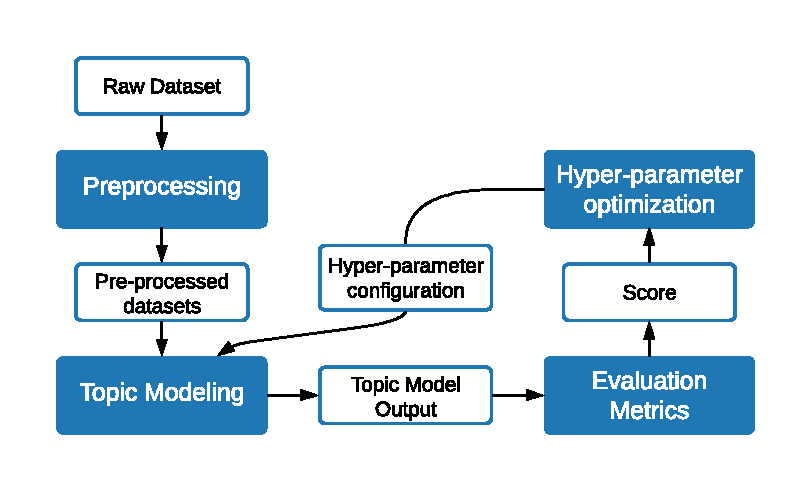
\includegraphics[width=0.7\textwidth]{images/octis.pdf}
%     \caption{Workflow of the OCTIS framework \cite{terragni_octis_2021}}
%     \label{fig:octis}
% \end{figure}

% OCTIS could be useful for the Master's thesis, as it provides a unified framework for training the proposed BERTopic model alongside the baseline models, facilitating their comparison across a variety of evaluation metrics. In fact, in the original BERTopic paper, \citet{grootendorst_bertopic_2022} employed OCTIS to evaluate the model's performance.

% \clearemptydoublepage

% \chapter{Literature Review}\label{chapter:literature_review}
% The goal of this chapter is to introduce the reader with the preliminary knowledge which is needed for understanding this research. We present an in-depth literature review of the current state-of-the-art and most widely adopted topic modeling techniques, along with the evaluation metrics used to assess the quality of the extracted topics. The foundational models discussed include Latent Dirichlet Allocation (LDA), Non-negative Matrix Factorization (NMF), and Top2Vec.

For the reader that is primarily interested in the approach that will be central to this research, we encourage you to focus on the subsection about BERTopic. As BERTopic will serve as the primary model in this research, the others — LDA, NMF, Top2Vec — will be used as baseline models for comparison.

Readers interested in a comprehensive overview of the field are invited to explore the broader literature in \cref{sec:broad_literature_review}, which provides a detailed account of topic modeling techniques, their applications and history.

\section{Latent Dirichlet Allocation}
% refer to section with broad literature review
Latent Dirichlet Allocation (LDA) \cite{blei_latent_2001} is a seminal and widely adopted generative probabilistic model that assumes documents are a mixture of topics, and topics are a mixture of words. It is based on the bag-of-words assumption, i.e. the order of words in a document does not matter.

\Cref{fig:lda} illustrates the plate notation for LDA. Each plate can be viewed as a "loop", where the variable in the bottom right can be seen as the number of iterations of the loop. The figure shows that there are $K$ topics whose Dirichlet distribution over words is controlled by the hyper-parameter $\beta$. The plate below shows that there are $M$ documents, each of which has $N$ words. The gray circle with $w$ represents the observed word, while the other circles represent latent variables. $z$ refers to the topic of $w$, $\theta$ refers to the Dirichlet distribution of topics over documents, which is controlled by the hyper-parameter $\alpha$.

\begin{figure}[h] % adjust placement if needed
    \centering
    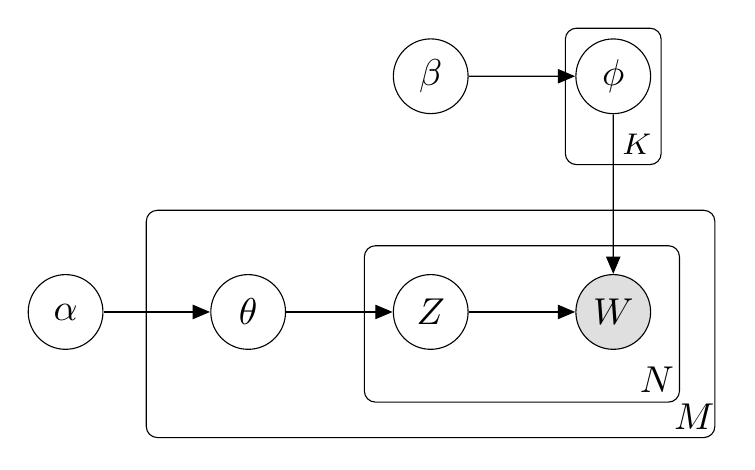
\begin{tikzpicture}[scale=1.35, transform shape]
        % Define nodes
        \node[obs]                               (w) {$W$};
        \node[latent, left=of w] (z) {$Z$};
        \node[latent, left=of z] (theta) {$\theta$};
        \node[latent, left=of theta]            (alpha) {$\alpha$};
        \node[latent, above=of w, yshift=0.5cm]            (phi) {$\phi$};
        \node[latent, left=of phi]              (beta) {$\beta$};

        % Connect the nodes
        \edge {z} {w} ;
        \edge {theta} {z} ;
        \edge {alpha} {theta} ;
        \edge {beta} {phi} ;
        \edge {phi} {w} ;

        % Plates
        \plate [inner sep=0.8cm] {plate1} {(theta)(z)(w)} {} ;
        \plate [inner sep=0.35cm] {plate2} {(w)(z)} {} ;
        \plate {plate3} {(phi)} {$K$} ;

        % Manually adjust label positions
        \node [xshift=-0.2cm, yshift=0.2cm] at (plate1.south east) {$M$};
        \node [xshift=-0.55cm, yshift=0.55cm] at (plate1.south east) {$N$};

    \end{tikzpicture}
    \caption{LDA plate notation}
    \label{fig:lda}
\end{figure}

The generative process for a corpus in the context of LDA is as follows:

\begin{enumerate}
    \item For each document $i = 1, \ldots, M$:
          \begin{itemize}
              \item Sample $\theta$ from a Dirichlet distribution $\theta_i \sim \text{Dir}(\alpha)$.
          \end{itemize}
    \item For each topic $k = 1, \ldots, K$:
          \begin{itemize}
              \item Sample $\phi$ from another Dirichlet distribution $\phi_k \sim \text{Dir}(\beta)$.
          \end{itemize}
    \item For each word $j = 1, \ldots, N$ in document $i$:
          \begin{itemize}
              \item Sample a topic $z_{ij} \sim \text{Multinomial}(\theta_i)$.
              \item Sample a word $w_{ij} \sim \text{Multinomial}(\phi_{z_{ij}})$.
          \end{itemize}
\end{enumerate}

$\theta_{ik}$ represents the probability of the $i$-th document to contain words from the $k$-th topic. Similarly, $\phi_{kw}$ represents the probability of the $k$-th topic to contain the $w$-th word.

\subsection{Dirichlet distribution}

Take the example of a large digital library of academic papers. First, for each paper $i$, we sample its topic distribution $\theta_i$ from a Dirichlet distribution. This represents the mixture of topics covered by the document. Secondly, for each topic $k$, we sample a word distribution $\phi_k$ over each topic from a Dirichlet distribution. Then, for each word $j$ in the document, we draw a topic $z_{ij}$ from the topic distribution Multinomial($\theta_i$), followed by sampling a word $w_{ij}$ from the word distribution Multinomial($\phi_{z_{ij}}$). This process models the generation of words in an academic paper based on latent topic structures and their corresponding word distributions.

The intuition behind the Dirichlet distribution is that the $k$-dimensional Dirichlet distribution $\theta$ is controlled by a $k$-dimensional vector of positive real numbers, $\alpha$. The $\alpha$ parameter shapes how topics are distributed across documents. A uniform $\alpha$ suggests no prior preference for topic prevalence, leading to a balanced mix of topics within documents. Smaller $\alpha$ values push the model towards sparser topic representations, where documents are likely to be dominated by fewer topics. An asymmetric $\alpha$ allows for the modeling of prior beliefs about topic prevalence, making some topics more prominent than others.

Similarly, $\beta$ controls the concentration of the word distribution for each topic, where the $m$-dimensional Dirichlet distribution $\phi$ is controlled by a $m$-dimensional vector of positive real numbers, $\beta$.

\subsection{Learning LDA}

The problem of learning an LDA model is referred to as an "inference" problem. That is, given the observed variable, \( w \), and the hyper-parameters \( \alpha \) and \( \beta \), how do we estimate the posterior of the latent variables:

\[ p(\theta, z, \phi | w, \alpha, \beta) = \frac{p(\theta, z, \phi, w | \alpha, \beta)}{p(w | \alpha, \beta)} \]

\citet{blei_latent_2001} discover that the integral for computing in the denominator is infeasible to compute exactly:

\[ p(w | \alpha, \beta) = \frac{\Gamma(\sum_i \alpha_i)}{\prod_i \Gamma(\alpha_i)} \int \left( \prod_i \theta_i^{\alpha_i - 1} \right) \left( \prod_{n=1}^{N} \prod_{i=1}^{k} \prod_{j=1}^{V} (\theta_i \beta_{ij})^{w_{n}} \right) d\theta \]

Therefore, approximate inference must be applied. Common approaches are Gibbs sampling and variational inference. Without delving into too much detail, Gibbs sampling allows us to avoid directly computing the intractable integral. The basic idea is that we want to sample from \(p(w \mid \alpha, \beta)\) to estimate the distribution, but we cannot directly do so. Instead, Gibbs sampling allows us to iteratively compute the posterior of one of the latent variables while fixing all the other variables. This way, we can obtain the posterior distribution \(p(\theta, z, \phi \mid w, \alpha, \beta)\).

For each iteration, we alternatively sample \(\theta\), \(z\), \(\phi\) with all the other variables fixed. Because the samples from the early iterations are not stable, we discard the first \(B\) iterations of samples. The algorithm is shown in the following pseudo code:


For \(i\) from \(1\) to \(\text{MaxIter}\):
\begin{itemize}
    \item Sample \(\theta_{i} \sim p(\theta \mid z = z_{i-1}, \phi = \phi_{i-1}, w, \alpha, \beta)\)
    \item Sample \(z_{i} \sim p(z \mid \theta = \theta_{i}, \phi = \phi_{i-1}, w, \alpha, \beta)\)
    \item Sample \(\phi_{i} \sim p(\phi \mid \theta = \theta_{i}, z = z_{i}, w, \alpha, \beta)\)
\end{itemize}

The algorithm begins with initial, possibly random, values for the variables \(\theta\), \(z\), and \(\phi\), and proceeds through a series of iterations up to a predefined maximum number, \(\text{MaxIter}\). At each iteration \(i\), the value of \(\theta_i\) is sampled from its conditional distribution given the current values of \(z\) and \(\phi\), denoted \(z_{i-1}\) and \(\phi_{i-1}\) to reflect their values from the previous iteration, alongside any observed data or parameters \(w\), \(\alpha\), and \(\beta\). Following this, \(z_i\) is updated based on the new \(\theta_i\) and the previous \(\phi_{i-1}\), and finally, \(\phi_i\) is sampled using the latest values of \(\theta_i\) and \(z_i\). This sequential updating of variables leverages the simpler conditional distributions to approximate the complex joint distribution. As the number of iterations increases, the algorithm converges, meaning the samples generated become representative of the target distribution.

\section{Non-negative Matrix Factorization}
 Non-negative Matrix Factorization (NMF) \cite{shahnaz_document_2006, kasiviswanathan_emerging_2011, yan_learning_2013} is a technique where an original matrix, consisting of non-negative values, is decomposed into two distinct matrices. The fundamental principle of NMF is that the product of these two matrices approximates the original matrix. This decomposition is a form of dimensionality reduction. The large original matrix typically represents a set of documents, with each document being a vector of words. The two resultant matrices in NMF are the word-topic matrix and the topic-document matrix. The topic-word matrix shows the association between topics and words, while the topic-document matrix shows the relationship between topics and individual documents.

\Cref{fig:nmf} illustrates the decomposition of a matrix \(A\) into two matrices \(W\) and \(H\). The matrix \(A\) is a non-negative matrix, and the matrices \(W\) and \(H\) are also non-negative. The product of \(W\) and \(H\) approximates \(A\). \(A\) represents the word-document matrix, where each row corresponds to a word and each column corresponds to a document. \(W\) represents the word-topic matrix, where each row corresponds to a word and each column corresponds to a topic. \(H\) represents the topic-document matrix, where each row corresponds to a topic and each column corresponds to a document.

\begin{figure}[h] % adjust placement if needed
    \centering
    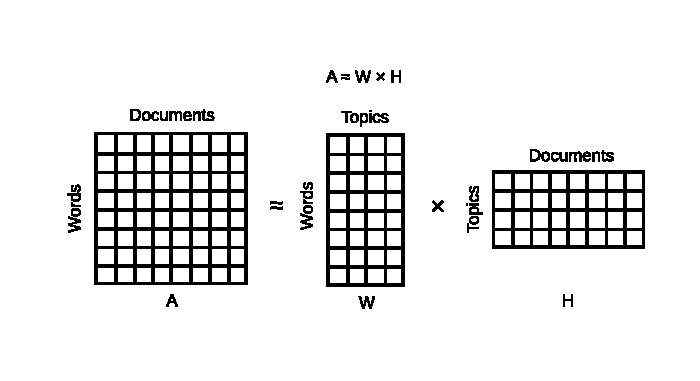
\includegraphics[width=0.75\textwidth]{figures/nmf.pdf}
    \caption{NMF decomposition}
    \label{fig:nmf}
\end{figure}

Non-negative Matrix Factorization is a group of algorithms whose objective is to minimize $F$ - the function which measures the error between the original matrix and the product of the two matrices. The most common algorithms for NMF typically involve iterative update rules that aim to minimize $F$, such as the Frobenius norm or the Kullback-Leibler (KL) divergence.

\subsection{Frobenius norm}

The goal in NMF using the Frobenius norm is to minimize the objective function \( F \), which is given by:

\[
    F = \| A - WH \|_F^2 = \sum_{i=1}^{n} \sum_{j=1}^{m} (A_{ij} - (WH)_{ij})^2
\]

where \( \| \cdot \|_F \) denotes the Frobenius norm. This objective function represents the sum of the squares of the element-wise differences between \( A \) and the product \( WH \).

The typical algorithm to minimize the Frobenius norm in NMF is an iterative process that involves:

\begin{enumerate}
    \item \textbf{Initialization:} Matrices \( W \) and \( H \) are initialized with non-negative values. This can be done randomly or based on some informed heuristic.
    \item \textbf{Iterative Update:} The matrices \( W \) and \( H \) are updated iteratively to reduce \( F \). The updates are performed using multiplicative rules that inherently maintain the non-negativity of \( W \) and \( H \). The update rules are as follows:
          \[
              W_{ai} \leftarrow W_{ai} \cdot \frac{(AH^\top)_{ai}}{(WHH^\top)_{ai}}
          \]
          \[
              H_{ib} \leftarrow H_{ib} \cdot \frac{(W^\top A)_{ib}}{(W^\top WH)_{ib}}
          \]
          where the indices \( a \) and \( b \) iterate over all rows and columns of \( W \) and \( H \), respectively.
    \item \textbf{Convergence:} The iteration continues until the change in \( F \) between successive iterations is less than a predetermined threshold, or a maximum number of iterations has been reached.
\end{enumerate}

While the Frobenius norm-based NMF is not convex over both \( W \) and \( H \) together, it is convex over each one individually when the other is held constant. Thus, each iteration is guaranteed to not increase \( F \), although the solution may converge to a local minimum rather than a global minimum.

\subsection{Kullback-Leibler}

Unlike the Frobenius norm which assesses the difference based on squared errors, the KL divergence is more suitable for data that is inherently probabilistic. The KL divergence for two matrices is defined as:

\[
    D(A || WH) = \sum_{i=1}^{n} \sum_{j=1}^{m} \left( A_{ij} \log\frac{A_{ij}}{(WH)_{ij}} - A_{ij} + (WH)_{ij} \right)
\]

where \( D(A || WH) \) represents the KL divergence between \( A \) and \( WH \), with the objective to minimize this divergence in NMF.

The iterative update rules for the matrices \( W \) and \( H \) that minimize the KL divergence are as follows:

\[
    W_{ai} \leftarrow W_{ai} \cdot \frac{(A \oslash (WH)H^\top)_{ai}}{\mathbf{1}H^\top_{ai}}
\]

\[
    H_{ib} \leftarrow H_{ib} \cdot \frac{(W^\top(A \oslash (WH)))_{ib}}{W^\top\mathbf{1}_{ib}}
\]

Here, \( \oslash \) denotes element-wise division, and \( \mathbf{1} \) is a matrix of ones that is used for normalization in the denominators.

Just like in the case of the Frobenius norm, the KL divergence-based NMF aims to iteratively update \( W \) and \( H \) until the decrease in \( D(A || WH) \) is below a certain threshold, signaling convergence. However, it is important to note that this optimization problem is non-convex, and the solution found may represent a local minimum.




\section{Top2Vec}
A limitation of LDA and NMF is that they disregard semantic relationships between words, thus neglecting context. As a result, text embedding techniques which capture context have become popular as an NLP technique.

\subsection{Embedding space (embeddings)}

In Top2Vec \cite{angelov_top2vec_2020}, the first step is to embed the documents into dense vector representations to capture the semantic meaning of the text. \Cref{fig:doc_word_embedding} \cite{angelov_top2vec_2020} illustrates the embedding space, where the purple dots represent words and the green dots represent documents. Words are closest to documents that contain them, and documents are closest to words that are most representative of their content.

\begin{figure}[h] % adjust placement if needed
    \centering
    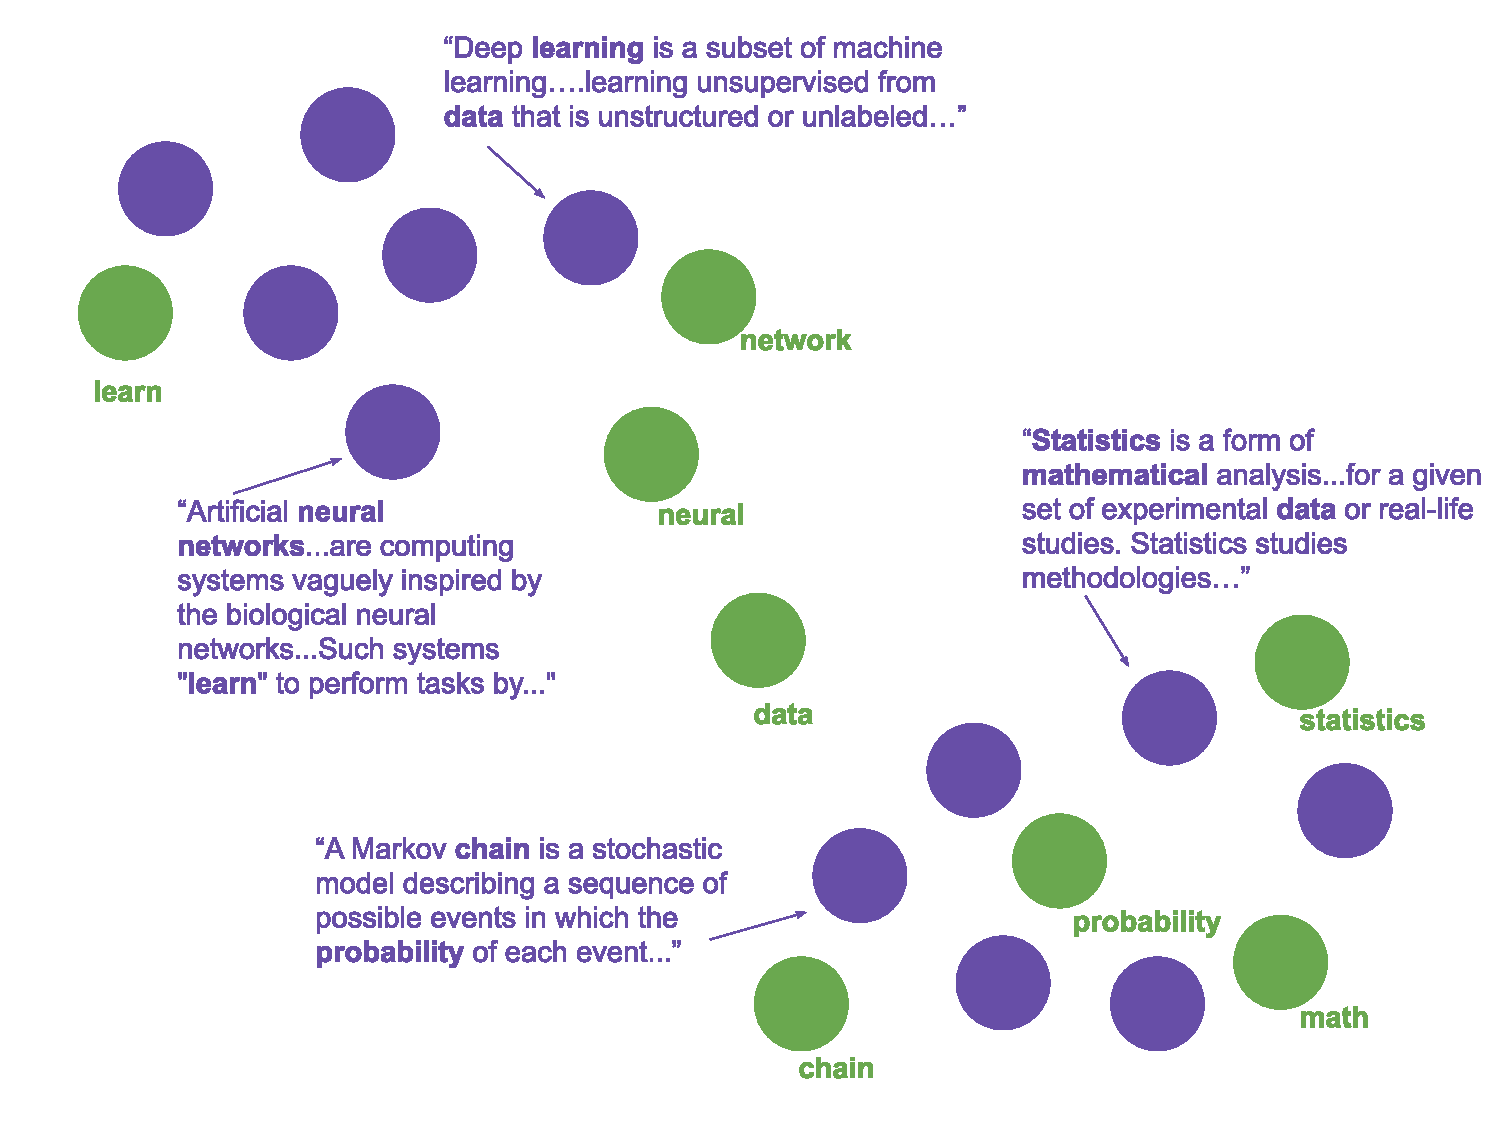
\includegraphics[width=0.65\textwidth]{figures/doc_word_embedding.pdf}
    \caption{Example of embedding space}
    \label{fig:doc_word_embedding}
\end{figure}

To learn the embedding space, Top2Vec utilizes Doc2Vec \cite{le_distributed_2014, rehurek_software_2010}, Universal Sentence Encoder \cite{cer_universal_2018}, or Sentence-BERT \cite{reimers_sentence-bert_2019}.

The original paper uses Doc2Vec's Distributed Bag of Words (DBOW) model, and even though it is simpler than Doc2Vec's Distributed Memory (DM) model, it is more efficient and has been shown to perform better in practice \cite{lau_empirical_2016}. DBOW essentially uses the document vector to predict words within a context window in the document.

Doc2Vec's DBOW is similar to Word2Vec's Skip-gram model (\cref{sec:word_embedding_topic_models}), which uses the context word to predict surrounding words in the context window. The difference is that DBOW switches the context word for the document vector to predict the surrounding words in the context window.

The process of learning the embedding space in Top2Vec can be summarized as follows:
\begin{enumerate}
    \item \textbf{Matrix Initialization}: The process initiates with the establishment of two matrices. The document matrix, denoted as $D_{c,d}$, encapsulates document vectors where $c$ represents the corpus's document count and $d$ the embedding dimensionality. Each row within $D_{c,d}$ represents a distinct document vector $\vec{d} \in \mathbb{R}^d$. Concurrently, the context word matrix $W'_{n,d}$, representing word vectors in analogous $d$-dimensional space for $n$ vocabulary words, may originate from pre-training, random initialization, or parallel learning processes.

    \item \textbf{Word Prediction Mechanism}: Contrary to relying on neighboring context words for prediction, the DBOW model employs the document vector for prediction. For every document $d$, each word's context vector $\vec{w_c}'$ within $d$ (sourced from $W'_{n,d}$) aids in inferring the document's vector $\vec{d}$ in $D_{c,d}$. This inference employs a softmax function, $\text{softmax}(\vec{w_c}' \cdot D_{c,d})$, generating a corpus-wide probability distribution reflecting each document's likelihood of generating the word.

    \item \textbf{Learning Process}: The learning process aims to optimize the document and word vectors to predict the document's constituent words. This optimization leverages backpropagation and stochastic gradient descent to modify both $D_{c,d}$ and $\vec{w_c}'$ from $W'_{n,d}$ to maximize the probability $P(\vec{d} | \vec{w})$ of correctly predicting the document given its words.

    \item \textbf{Embedding Space}: Through optimization, an embedding space emerges where documents gravitate towards the vectors of words they comprise, effectively "attracted" by these words. Consequently, semantically similar documents (sharing similar words) cluster, whereas dissimilar documents (sharing fewer words) diverge.
\end{enumerate}

\subsection{Number of topics}

In the embedding space, a dense area of documents can be interpreted as an area of highly similar documents. First, Uniform Manifold Approximation and Projection for Dimension Reduction (UMAP) \cite{mcinnes_umap_2020} is used to reduce the dimensionality of the document vectors. That is because the high-dimensional document vectors lead to the "curse of dimensionality", where the document vector sparsity makes it difficult to find dense clusters. Then, in order find the dense areas of documents in the embedding space, density-based clustering is used on the document vectors, specifically Hierarchical Density-Based Spatial Clustering of Applications with Noise (HDBSCAN) \cite{campello_density-based_2013, mcinnes_accelerated_2017, mcinnes_hdbscan_2017}. HDBSCAN assigns a label to each dense cluster of document vectors and assigns a noise label to all document vectors that are not in a dense cluster.


\subsection{Topic vectors}

Given labels for each cluster of dense documents in the embedding space, topic vectors can be calculated. The authors lay out multiple methods for calculating topic vectors, but discover that they perform similarly. The method that is used in the original paper is to calculate the centroid of the document vectors in each cluster. The centroid is the average of all the document vectors in the cluster. The centroid is calculated for each set of document vectors that belong do a dense cluster, generating a topic vector for each set. The number of dense areas found is the number of prominent topics identified in the corpus.

In the embedding space, every point represents a topic that is best described semantically by its nearest word vectors. Therefore, the word vectors that are closest to a topic vector are those that are most representative of it semantically. The distance of each word vector to the topic vector will indicate how semantically similar the word is to the topic. The words closest to the topic vector can be seen as the words that are most similar to all documents into the dense area, as the topic vector is the centroid of that area. These words can be used to summarize the common topic of the documents in the dense area.

\section{BERTopic}
Top2Vec simplifies the process of generating topics by clustering embeddings of words and documents. Inspired from Top2Vec, BERTopic \cite{grootendorst_bertopic_2022} is a state-of-the-art topic model that builds on top of the clustering embeddings approach. It employs a variation of c-TF-IDF for classes to generate representations of topics.


BERTopic generates representations of topics through a six-step process. Initially, it transforms each document into an embedding using a pre-trained language model. Before the clustering process, the dimensionality of these embeddings is reduced. Following this, the embeddings are clustered. Subsequently, a bag-of-words representation is generated for each cluster, containing the frequency of every word. Next, topic representations are derived from these clusters using a specialized class-based version of TF-IDF. The final step optionally fine-tunes these topic representations.


While these steps are the default, BERTopic offers a degree of modularity. Each step in the process is relatively independent from the others. For instance, the tokenization step does not depend on the specific embedding model used for document conversion, which provides flexibility in how tokenization is executed.

This flexibility is particularly important during the clustering step. Clustering models such as HDBSCAN are built on the premise that clusters can vary in shape and form. Consequently, employing a centroid-based technique for modeling topic representations may not be appropriate, as the centroid may not accurately reflect the nature of these clusters. In contrast, a bag-of-words approach assumes minimal knowledge about the cluster's shape and form.

As a result, BERTopic is highly modular, maintaining its ability to generate topics across different sub-models. This means that BERTopic effectively allows for the construction of customized topic models. \Cref{fig:modularity_modified} (inspired by \cite{grootendorst_algorithm_nodate}) illustrates the six steps of BERTopic, presented from bottom to top. It highlights the possibility of employing various techniques at each step of the process. For example, one could choose between SBERT or spaCy for document embedding, UMAP or PCA for dimensionality reduction, and GPT or KeyBERT \cite{grootendorst_maartengrkeybert_2024} for the fine-tuning phase.

\begin{figure}[h] % adjust placement if needed
    \centering
    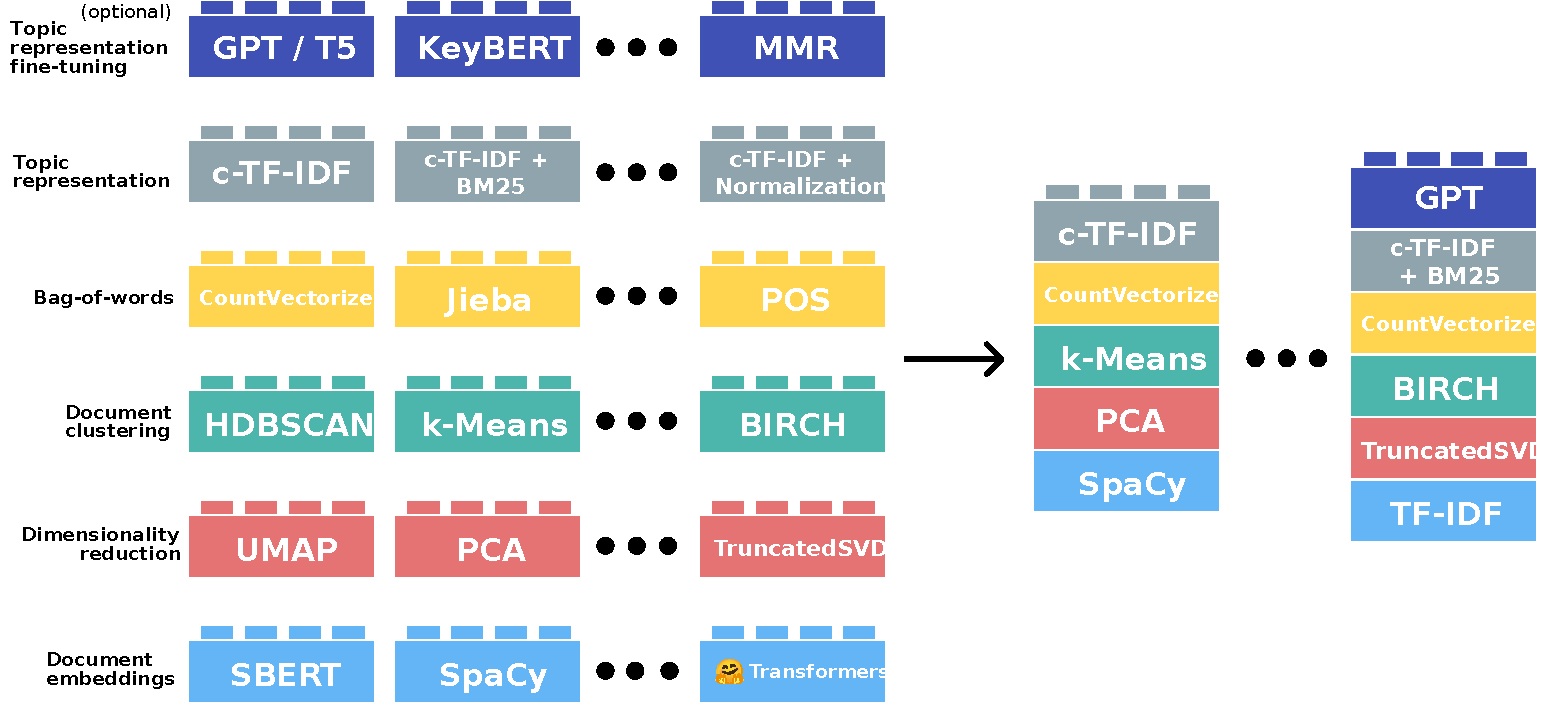
\includegraphics[width=\textwidth]{figures/modularity_modified.pdf}
    \caption{BERTopic modularity}
    \label{fig:modularity_modified}
\end{figure}

\subsection{Document embeddings}

In BERTopic, documents are transformed into embeddings to create vector space representations for semantic comparison. It is based on the idea that documents sharing the same topic will have similar semantics. For this embedding step, BERTopic utilizes the SBERT framework \cite{reimers_sentence-bert_2019}. SBERT enables the conversion of sentences and paragraphs into dense vector representations by employing pre-trained language models. This achieves top performance on several sentence embedding tasks \cite{reimers_making_2020}. The embeddings are mainly used for clustering documents with semantic similarities rather than directly for topic generation. BERTopic can use any embedding technique, provided the language model used for generating document embeddings is fine-tuned for semantic similarity. Hence, the quality of BERTopic's clustering improves as more advanced language models are developed, allowing BERTopic to evolve alongside advancements in embedding techniques. This proves particularly useful in the context of topic modeling, since the quality of the embeddings directly influences the quality of the topics generated.

\textbf{Expand on embedding models}

\subsection{Dimensionality reduction}

As the dimensionality of data increases, the distance to the nearest data point tends to become similar to the distance to the farthest data point \cite{aggarwal_surprising_2001, beyer_when_1999}. This phenomenon implies that in high-dimensional spaces, the notion of spatial locality becomes unclear, and distances between points show minimal variation. While several clustering methods have been developed to address this curse of dimensionality \cite{pandove_systematic_2018, steinbach_challenges_2004}, a simpler strategy involves reducing the dimensionality of embeddings. Although PCA and t-SNE are popular dimensionality reduction techniques, UMAP \cite{mcinnes_umap_2020} has been found to better preserve the local and global characteristics of high-dimensional data in its lower-dimensional representations \cite{mcinnes_umap_2020}. Furthermore, UMAP's flexibility regarding the dimensions of embeddings allows its application across various embedding models.

\textbf{Expand on details for UMAP}
\subsection{Document clustering}

The reduced embeddings are clustered using a clustering model/algorithm. A popular choice is HDBSCAN \cite{campello_density-based_2013, campello_hierarchical_2015, mcinnes_accelerated_2017, mcinnes_hdbscan_2017}. HDBSCAN is built on top of DBSCAN \cite{ester_density-based_nodate} and is designed to identify clusters of various densities by transforming DBSCAN into a hierarchical clustering algorithm. It employs a soft-clustering approach, which allows for the treatment of noise as outliers. Traditional clustering assigns each point in a dataset to a cluster, which is a hard assignment without mixed memberships. Conversely, in soft clustering, points are not assigned a cluster label, but are instead assigned a vector of probabilities. This allows points to potentially be a mix of clusters. Soft clustering is particularly useful in topic modeling, as documents can belong to multiple topics.

Furthermore, \citet{allaoui_considerably_2020} showed that the performance of well-known clustering algorithms, including k-Means and HDBSCAN, can be significantly improved by reducing the dimensionality of high-dimensional embeddings with UMAP, in terms of both clustering accuracy and computational time.
\textbf{Expand on details for HDBScan}

\subsection{Bag-of-words}

Before creating topic representations in BERTopic, it is necessary to select a technique that supports the algorithm's modular nature. When using HDBSCAN, we assume that clusters may vary in density and shape, indicating that techniques based on centroid models may not be suitable. The desired method should ideally make minimal assumptions about the cluster structures.

The process begins by combining all documents within a cluster into a single document, which then represents the entire cluster. Subsequently, the frequency of each word within this single document is counted, resulting in a bag-of-words representation that reflects the word frequencies at the cluster level rather than the individual document level. The adoption of a bag-of-words approach ensures that no assumptions are made about the density and shape of the clusters.

There are various approaches to constructing a bag-of-words representation, facilitated by the use of \texttt{CountVectorizer}. \texttt{CountVectorizer} allows us to control the number of tokens in each topic representation. For instance, single words like \textit{game} or \textit{team} may appear in a topic, but it can also be useful to include multi-word phrases, such as \textit{hockey league}, which consist of two tokens. Additionally, some topics might include stop words, such as \textit{he} or \textit{the}, which are generally undesirable in topic representations as they provide little meaningful information. Removing these stop words is typically preferred to improve the quality of the topics.

\subsection{Topic representation}
From the generated bag-of-words representation, our goal is to identify what distinguishes one cluster from another. Specifically, we want to determine which words are characteristic of a particular cluster (e.g., cluster 1) but less common in other clusters. To achieve this, we need to modify the traditional TF-IDF such that it operates at the cluster level, treating clusters as topics instead of individual documents.

The classic TF-IDF \cite{joachims_probabilistic_1997} method combines term frequency and inverse document frequency to calculate a weight $W_{t,d}$ for term $t$ in document $d$ as follows:

\[ W_{t,d} = tf_{t,d} \cdot \log\left(\frac{N}{df_t}\right) \]

Here, term frequency $tf_{t,d}$ represents the frequency of term $t$ in document $d$, and inverse document frequency measures $t$'s importance across documents, calculated by the logarithm of the ratio of the total number of documents $N$ to the number of documents containing $t$.


BERTopic extends the TF-IDF concept to clusters of documents by introducing class-based TF-IDF (c-TF-IDF). In this approach, documents within a cluster are concatenated into a single document, and the TF-IDF formula is modified for cluster-level representation:

\[ W_{t,c} = tf_{t,c} \cdot \log\left(1 + \frac{A}{tf_t}\right) \]

In this formula, term frequency $tf_{t,c}$ now models the frequency of term $t$ within a cluster $c$, treated as a single document. The inverse document frequency is substituted with an inverse class frequency, which assesses the term's importance to a cluster. This is calculated by the logarithm of the average number of words per cluster $A$ divided by the term's frequency $tf_t$ across all clusters, with $1$ added inside the logarithm to ensure positive values. This adaptation of TF-IDF to clusters allows us to model the importance of words in clusters instead of individual documents. Furthermore, by iteratively merging c-TF-IDF representations of less prevalent topics with their closest topics, the total number of topics can be reduced to meet a predefined threshold.

\subsection{(Optional) Topic representation fine-tuning}

After generating the c-TF-IDF representations, we obtain a collection of words that describe a collection of documents. c-TF-IDF is a method for quickly producing accurate topic representations. Nonetheless, the field of NLP is rapidly advancing, with frequent new developments. To make use of these developments, BERTopic offers the option to refine c-TF-IDF topics further using GPT \cite{radford_improving_nodate, radford_language_nodate, brown_language_2020}, KeyBERT \cite{grootendorst_maartengrkeybert_2024}, spaCy \cite{noauthor_explosionspacy_nodate}, and other techniques, many of which are integrated within the BERTopic library. Users can also implement their own fine-tuning methods, allowing for a high degree of customization.

In particular, the topics generated through c-TF-IDF can be viewed as canditate topics, comprising a set of terms and representative documents. These can serve as a foundation for further refinement of topic representations. The availability of representative documents for each topic can be useful, as it enables fine-tuning on a reduced number of documents, thereby reducing computational demands. This makes the use of architectures such as large language models more viable in production environments, often resulting in shorter processing times compared to the steps of dimensionality reduction and clustering.

\subsection{Evaluation metrics}

% According to \citet{abdelrazek_topic_2022}, topic models, which are applicable across a variety of domains, can undergo evaluation through two distinct approaches: extrinsic and intrinsic. Extrinsic evaluation assesses performance based on the specific domain of application, whereas intrinsic evaluation focuses on the qualities of the generated topics themselves, independent of any domain. This makes intrinsic evaluation more universally applicable. The various models are distinguished by their simplicity, computational efficiency, and underlying assumptions, which influence their performance across different corpora and applications. However, there is a lack of agreement on the criteria for evaluating topic models, and multiple methods exist for evaluating the same quality.

% \citet{abdelrazek_topic_2022} highlight a range of criteria for evaluating topic models, including quality, interpretability, stability, diversity, efficiency, and flexibility, as illustrated in \cref{fig:evaluation_criteria}. We will focus on quality, interpretability, and diversity, given their relevance to our specific use case.

% \begin{figure}[h] % adjust placement if needed
%     \centering
%     \begin{tikzpicture}
%         \node (eval) [rectangle, draw, text width=3cm, text centered, minimum height=0.75cm] {Evaluation metrics};

%         \node (quality) [rectangle, draw, below left=of eval, text width=2cm, text centered, minimum height=0.75cm, xshift=-3.35cm, yshift=0.5cm] {Quality};
%         \node (interpretability) [rectangle, draw, right=of quality, text width=2cm, text centered, minimum height=0.75cm, xshift=-0.41cm] {Interpretability};
%         \node (stability) [rectangle, draw, right=of interpretability, text width=2cm, text centered, minimum height=0.75cm, xshift=-0.41cm] {Stability};
%         \node (diversity) [rectangle, draw, right=of stability, text width=2cm, text centered, minimum height=0.75cm, xshift=-0.41cm] {Diversity};
%         \node (efficiency) [rectangle, draw, right=of diversity, text width=2cm, text centered, minimum height=0.75cm, xshift=-0.41cm] {Efficiency};
%         \node (flexibility) [rectangle, draw, right=of efficiency, text width=2cm, text centered, minimum height=0.75cm, xshift=-0.41cm] {Flexibility};

%         \draw[-] (eval.south) -- ++(0,-0.25) -| (quality.north);
%         \draw[-] (eval.south) -- ++(0,-0.25) -| (interpretability.north);
%         \draw[-] (eval.south) -- ++(0,-0.25) -| (stability.north);
%         \draw[-] (eval.south) -- ++(0,-0.25) -| (diversity.north);
%         \draw[-] (eval.south) -- ++(0,-0.25) -| (efficiency.north);
%         \draw[-] (eval.south) -- ++(0,-0.25) -| (flexibility.north);
%     \end{tikzpicture}
%     \caption{Topic models evaluation criteria \cite{abdelrazek_topic_2022}}
%     \label{fig:evaluation_criteria}
% \end{figure}

% \textbf{Quality and Perplexity}

% Perplexity measures a model's ability to reproduce the documents in a corpus using the learned topics. It evaluates the model's predictive ability rather than its ability to uncover the latent structure, indicating how effectively the model explains the data. A lower perplexity suggests a model is more effective in explaining the observed documents, as it implies a higher information gain from predicting the outcome of the random variable.

% However, using perplexity as an evaluation metric for our use case has several drawbacks. Firstly, perplexity needs to be normalized for the size of the corpus vocabulary, as it varies with different corpus and topic sizes. This is a consideration especially since BERTopic may not consistently extract the same number of topics without specific instructions to limit topic quantity. Additionally, perplexity has not been found to be correlated with human judgment \cite{chang_reading_2009}. Furthermore, non-generative models like NMF do not have a defined perplexity score because they do not provide probabilities of word sequences.

% \textbf{Interpretability and Topic coherence}

% A topic is defined as a discrete distribution over words, with the expectation that this word set is interpretable by humans. For interpretability, the words generated should collectively convey a single semantic meaning. Topic coherence metrics evaluate how related the top-k words of a topic are to one another.

% \citet{newman_automatic_2010} measure coherence by examining the lexical similarity between word pairs, employing various similarity measures and identifying mutual information as the most reliably performing measure. The pointwise mutual information, $PMI$, between a pair of words $(w_i, w_j)$ is calculated as follows:

% \[PMI(w_i, w_j) = \frac{\log p(w_i, w_j)}{p(w_i)p(w_j)}\]

% This formula quantifies the difference between the probability of $w_i$ and $w_j$ occurring together compared to the probabilities of them appearing independently within the corpus. Here, $p(w_i,w_j)$ represents the joint probability of both words occurring together, while $p(w_i)$ and $p(w_j)$ are the individual probabilities $w_i$ and $w_j$ occurring in the corpus.

% A known trade-off exists between coherence and perplexity \cite{chang_reading_2009}, where optimizing for lower perplexity often results in decreased coherence.

% \textbf{Topic diversity}

% Topic diversity refers to the semantic diversity among the generated topics. A method to assess diversity, as proposed by \citet{dieng_topic_2020}, considers it as the proportion of unique words within the top 25 words across all topics. So, in general, diversity metrics aim to quantify the variation among the top-k words within a topic. A high score in topic diversity suggests that a topic model successfully generates diverse topics, whereas a low score may indicate the presence of redundant topics, showing the model's inability to clearly differentiate the themes within the corpus. It is important to note that the choice of the number of topics in a model significantly influences topic diversity. Choosing too many topics might lead to similar topics with overlapping words, while too few topics can result in overly broad topics that lack interpretability.

% \textbf{Classification evaluation metrics}

% The evaluation metrics discussed previously pertain to topic modeling as an unsupervised learning task. If through experimentation we establish that the BERTopic model underperforms, we might approach the problem as a (semi-)supervised task, in which case different evaluation metrics would be used. Beyond well-known metrics such as accuracy, precision, recall, and F1 score, coverage and purity would also be considered \cite{churchill_evolution_2022}.

% Coverage examines the extent to which the concepts within the document collection are captured by the model. It can be divided into topic coverage and document coverage. Topic coverage measures how good the model is at identifying the topics in a document corpus. The most popular measure for topic coverage is topic recall, which denotes the proportion of ground truth topics identified by the topic model. Conversely, document coverage focuses on how well documents are represented by the topics. Topic model accuracy is a frequently used measure, which is the proportion of documents accurately labeled by the model. For evaluating both topic recall and accuracy, ground truth topics are required.

% When ground truth topics are missing, alternative metrics like purity are used. Purity measures the model's accuracy under the assumption that documents are always assigned to the dominant topic. This metric aims to penalize models that assign a large number of low probability topics to documents, in contrast to models that assign a high probability to a single topic from the document corpus.

% \textbf{OCTIS}

% OCTIS (Optimizing and Comparing Topic models Is Simple) \cite{terragni_octis_2021} is an open-source framework for the training, analysis, and comparison of topic models across various datasets and evaluation metrics.

% It allows for the optimization of model hyper-parameters for experimental comparison. OCTIS introduces a pipeline for topic modeling (\cref{fig:octis}), which includes dataset preprocessing, training topic models, evaluation metrics, hyperparameter optimization, and visualization through an interactive web dashboard.

% OCTIS offers a range of evaluation metrics for assessing topic models, such as coherence, significance, diversity, and classification metrics.

% The discovery of optimal hyper-parameter settings relies on a Bayesian Optimization (BO) approach \cite{archetti_bayesian_2019, galuzzi_hyperparameter_2020, snoek_practical_2012}, where the objective can be any of the available evaluation metrics. Given the potential variability in performance outcomes due to noise, the objective function is defined as the median performance across multiple runs of the model under the same hyperparameter settings for the chosen evaluation metric.

% BO is a sequential, model-based optimization technique for noisy black-box functions that are costly and complex to evaluate directly, such as topic models. Its main idea involves using all previously evaluated hyperparameter settings to approximate the performance metric's value, and then selecting new, likely better hyperparameter settings for the next run. The approximation is done by a probabilistic \textit{surrogate model}, which has a prior belief of the objective function based on observed hyperparameter settings. The selection of the next hyperparameter settings is driven by optimizing an \textit{acquisition function}, which uses the uncertainty within the posterior distribution to guide the exploration of the parameter space.

% \begin{figure}[h] % adjust placement if needed
%     \centering
%     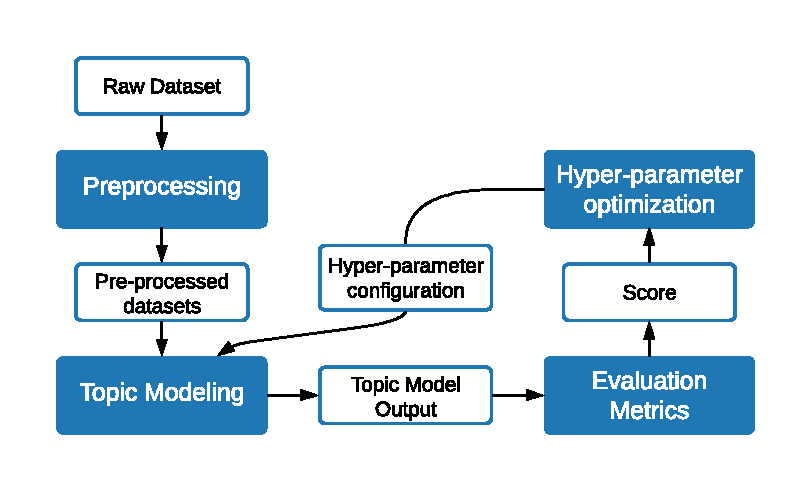
\includegraphics[width=0.7\textwidth]{images/octis.pdf}
%     \caption{Workflow of the OCTIS framework \cite{terragni_octis_2021}}
%     \label{fig:octis}
% \end{figure}

% OCTIS could be useful for the Master's thesis, as it provides a unified framework for training the proposed BERTopic model alongside the baseline models, facilitating their comparison across a variety of evaluation metrics. In fact, in the original BERTopic paper, \citet{grootendorst_bertopic_2022} employed OCTIS to evaluate the model's performance.

% \clearemptydoublepage

\chapter{Methodology}\label{chapter:methodology}
In this chapter, we present our proposed methodology, including the methods and techniques used to address our research questions. We also cover our data exploration and preprocessing steps, the hyperparameter tuning process, and the automated and human evaluation methods and metrics we have chosen.

\section{Data exploration, preprocessing and augmentation}
\subsection{Exploratory data analysis}
First, an exploratory data analysis (EDA) will be conducted to understand the characteristics of the OpenML dataset descriptions. This analysis will be unstructured, discovering patterns in the data in an exploratory manner, using statistical and visual methods. The goal of the EDA is to gain insights into the dataset descriptions, such as their length, vocabulary, distribution of words, etc. This information will help us understand the nature of the data and identify any preprocessing steps that may be necessary to improve the quality of the descriptions.

\subsection{Data preprocessing}
After the EDA, the dataset descriptions will undergo preprocessing to prepare them for the topic modeling process. This preprocessing may involve steps such as stemming, lemmatization, stop-word removal, and tokenization. These steps are important to ensure that the descriptions are in a suitable format for the topic modeling algorithms.

\subsection{Data augmentation}
In addition to the original dataset descriptions, we will explore the possibility of augmenting the data with additional information. This could include metadata such as dataset name, tags, features (column names), scraping from the original dataset if available, etc. This additional information can provide context and background to the descriptions, which may help improve the quality of the topics extracted by the topic model.

\section{Tag generation}
\label{sec:tag_generation}
In this subsection, we introduce our model, which is, in fact, a pipeline comprising multiple submodels and techniques. Steps 1-3 involve data preprocessing to prepare the data for the model. Steps 5-8 are referred to as the \textit{Base BERTopic model}. It includes dimensionality reduction, clustering, bag-of-words and c-TF-IDF. Finally, steps 9 and 10 represent our improvements to the base model, introducing an approach that, to the best of our knowledge, is novel within the literature. Additionally, we provide an explanation of which steps are computationally efficient and which are more expensive.

\begin{figure}[h]
    \centering
    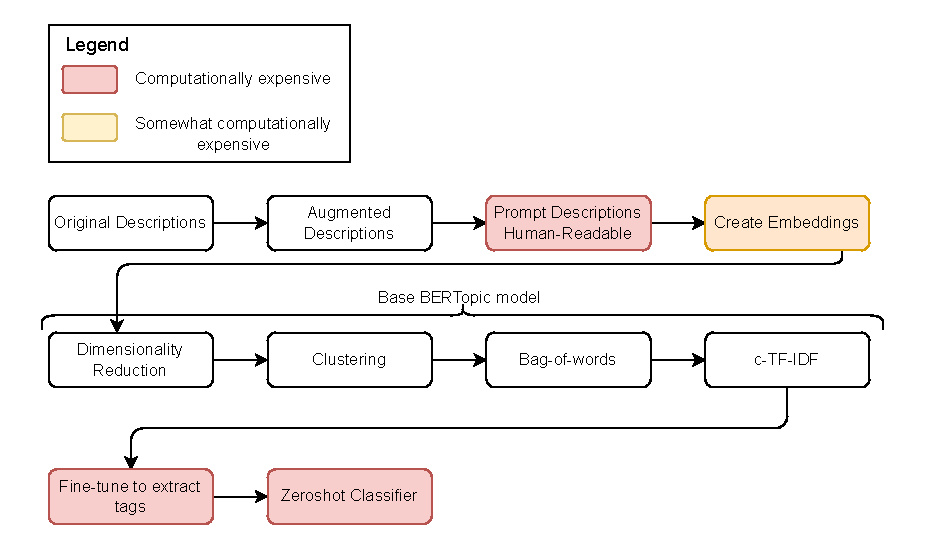
\includegraphics[width=\textwidth]{figures/tag_generation_pipeline.pdf}
    \caption{Tag generation pipeline}
    \label{fig:tag_generation_pipeline}
\end{figure}

To explain the pipeline illustrated in \cref{fig:tag_generation_pipeline} in more detail, we provide a step-by-step description of the process:

\begin{enumerate}
    \item \textbf{Original Descriptions}: The input to the pipeline is a set of original dataset descriptions. These come from the OpenML dataset and are used as the basis for generating tags.
    \item \textbf{Augmented Descriptions}: The OpenML dataset descriptions come with metadata such as dataset name, tags, features (column names) and some of them link to the original dataset, which can be used to scrape (extract) additional information. These are used to augment the dataset descriptions.
    \item \textbf{Prompt Descriptions Human-Readable}: Augmented descriptions are rewritten to be more human-readable via an LLM and prompt engineering. This is because the original descriptions are often in a technical format that is not easily interpretable by humans. Since LLMs are trained on large text corpora, they work best with human-readable (natural language) text.
    
    Additionally, we design the prompt to extract \textit{keyword tags} from each individual description. These tags are directly mentioned within the description and are typically highly specific to it. For instance, if a description includes the terms "US elections," "voting," and "candidates," these would be considered keyword tags.

    \item \textbf{Create Embeddings}: Embeddings for each description are created using a pre-trained embedding model.
    \item \textbf{Dimensionality Reduction}: The dimensionality of the embeddings is reduced to cure the curse of dimensionality.
    \item \textbf{Clustering}: The reduced embeddings are clustered to group similar descriptions together. The output of this step is clusters, which represent our topics. Each cluster contains a set of descriptions (which we now call \textit{representative documents}) that are similar to each other.
    \item \textbf{Bag-of-words}: The descriptions in each cluster are converted to a bag-of-words representation, ignoring common words such as "the", "and", etc.
    \item \textbf{c-TF-IDF}: The bag-of-words representation is used to calculate the c-TF-IDF score for each word in each cluster. This score is used to rank the words in each cluster.
    \item \textbf{Fine-tune to extract tags}: For each topic, we have representative documents (from the clustering step) and representative words (from the c-TF-IDF step). We prompt engineer a question that asks an LLM to generate tags for each cluster. The generated tags are categorized as \textit{regular tags} and \textit{overarching tags}.

    \textit{Regular tags} refer to tags that frequently appear among the representative documents and words. \textit{Overarching tags} capture the broader, more general theme of the cluster. For example, if a cluster pertains to "US elections" and the representative documents contain the word "election" while the representative words include "candidate", a possible regular tag could be "election candidate", whereas the overarching tag might be "politics".

    As context, we feed the LLM with the top \textit{k} representative documents and the top \textit{m} representative words for each topic. This results in tags that are common among the representative documents and representative words, and hence are representative of the topic.
    \item \textbf{Zeroshot Classifier}: Each description can in reality be contained in multiple clusters (topics). In this step, we get the top \textit{n} most likely clusters for each description. Then, for each description, we get the tags for each of the top \textit{n} clusters in a set. We feed this set of tags to a zeroshot text classification model, which returns confidences from 0 to 1 for whether each tag describes the description. This step is crucial for filtering out irrelevant tags for each description. For instance, if a description about diabetes and a description about cancer are both contained in the same topic (which may be, for example, "medical conditions"), we want to ensure that the tags for the cancer description are not assigned to the diabetes description. Furthermore, the description about diabetes may be contained in another topic that cancer is not in, such as "nutrition". In this case, we want to ensure that the tags in "nutrition" are not assigned to the cancer description, but are assigned to the diabetes description.

\end{enumerate}


\section{Automated evaluation metrics and baselines}
In order to evaluate the quality of the extracted topics, we will use a combination of automated evaluation metrics and baselines. These metrics and baselines will help us assess the performance of our model and compare it to existing topic modeling techniques. The following sections provide an overview of the metrics and baselines we will use in our evaluation.

\subsection{Metrics}
\subsubsection{Topic coherence}
As explained in \cref{sec:topic_coherence}, topic coherence is a widely used metric for evaluating the quality of topics generated by topic models. It measures the semantic similarity between words in a topic and is based on the assumption that coherent topics contain words that are related to each other. We will use topic coherence to assess the quality of the topics extracted by our model.

\subsubsection{Topic diversity}
Topic diversity (\cref{sec:topic_diversity}) is another important metric for evaluating topic models. It measures the extent to which topics are distinct from each other and do not overlap in terms of the words they contain. A diverse set of topics ensures that the model captures a wide range of themes and concepts present in the data. We will use topic diversity to evaluate the diversity of topics generated by our model.

\subsubsection{Silhouette score}
The silhouette score (\cref{sec:silhouette_score}) is a metric used to evaluate the quality of clusters in unsupervised learning. It measures how similar an object is to its own cluster (cohesion) compared to other clusters (separation). A high silhouette score indicates that the clusters are well-separated and that the objects within each cluster are similar to each other. We will use the silhouette score to evaluate the quality of the clusters generated by our model.

\subsection{Baselines}
In addition to the proposed topic model, we will compare its performance against several baseline models. These baselines represent established or commonly used topic modeling techniques and will serve as a point of reference for evaluating the proposed model. The baselines we will consider include Latent Dirichlet Allocation (LDA), Non-negative Matrix Factorization (NMF), and Top2Vec (described in \cref{sec:latent_dirichlet_allocation,sec:non-negative_matrix_factorization,sec:top2vec}), and Contextualized Topic Models (CTM) \cite{bianchi_pre-training_2021, bianchi_cross-lingual_2021} which are a less popular, but still effective topic modeling approach. These models are widely used in the field of topic modeling and will provide a benchmark for evaluating the performance of our model.

\subsection{Automated evaluation pipeline}

\Cref{fig:data_pipeline} shows a flowchart of the automated evaluation pipeline, which contains the following sequential steps:

\begin{enumerate}

    \item \textbf{Data Fetching}: This is the first stage where dataset descriptions are downloaded from OpenML.

    \item \textbf{Data Preparation}: After fetching the data, the next step involves preparing it. This includes removing noise, correcting errors, augmenting it, and standardizing the format to prepare it for analysis. Data preparation ensures that the input to the topic model is of high quality, which is crucial for the success of the subsequent modeling steps. \\ The next step involves removing inadequate data points, such as excessively short descriptions and duplicates. Stop words are removed for models that require it (e.g., LDA). Additionally, the process includes stemming and lemmatization to normalize words to their base forms.

    \item \textbf{Topic Model}: In this step, the proposed topic model is applied to the prepared data. In this case, it will be BERTopic. We refer to it as the \textit{Base BERTopic model}.

    \item \textbf{Benchmark Models}: Concurrently with the proposed topic model, benchmark models are run. These models represent established or baseline approaches to topic modeling against which the performance of the proposed topic model is compared. This will involve baseline models such as LDA, NMF and Top2Vec.

    \item \textbf{Topic Labels}: The output from both the topic model and the benchmark models are sets of topics, represented by a cluster of words that are characteristic of a particular topic.

    \item \textbf{Evaluation}: Finally, the performances of the proposed topic model and benchmark models are evaluated. This includes comparing the topic coherence, diversity and silhouette score.

\end{enumerate}

\begin{figure}[h]
    \centering
    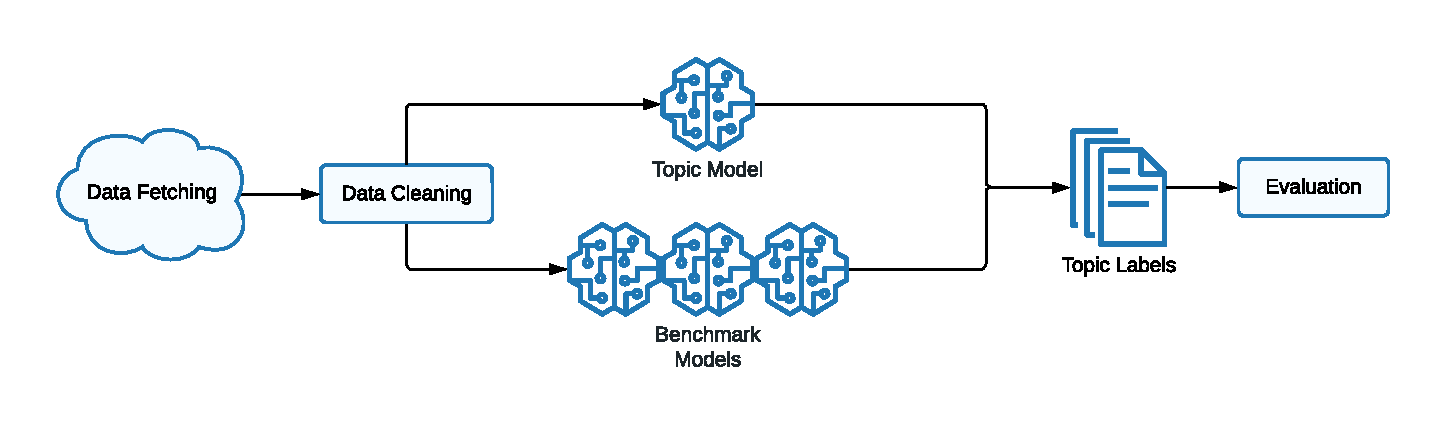
\includegraphics[width=\textwidth]{figures/data_pipeline.pdf}
    \caption{Data pipeline}
    \label{fig:data_pipeline}
\end{figure}

\subsection{Hyperparameter tuning}
\label{sec:hyperparameter_tuning}
As mentioned in \cref{sec:octis}, we will use Bayesian optimization to tune the hyperparameters of our \textit{Base BERTopic model}. This process will involve selecting the most relevant hyperparameters to optimize, defining the search space for each hyperparameter, and running the optimization algorithm to find the best combination of hyperparameters. The goal of hyperparameter tuning is to improve the performance of our model by finding the settings for the hyperparameters which are close to optimal.

As a metric to optimize, we will define a custom weighted metric which includes the topic coherence score and topic diversity score.

Let \( C \) represent the topic coherence score normalized between \([-1, 1]\), and \( D \) represent the topic diversity score normalized between \([0, 1]\). The normalized scores are given by:

\[
C_{\text{norm}} = \frac{C + 1}{2}, \quad D_{\text{norm}} = D
\]

We apply a log transformation to both scores. The log-transformed scores are defined as:

\[
\log(C_{\text{norm}} + \epsilon), \quad \log(D_{\text{norm}} + \epsilon)
\]

where \( \epsilon = 10^{-10} \) is a small constant to avoid undefined values at zero.

Finally, the weighted metric \( M \) is computed as:

\[
M = w_C \cdot \log(C_{\text{norm}} + \epsilon) + w_D \cdot \log(D_{\text{norm}} + \epsilon)
\]

where \( w_C \) and \( w_D \) are the weights for coherence and diversity, respectively.

The log transformation is applied to both the coherence and diversity scores for several reasons. First, it helps to handle skewed distributions by compressing large values and expanding smaller ones, which ensures that extreme values do not dominate the final metric. This makes the scores more comparable. Additionally, the log transformation avoids issues with zero values by introducing a small constant \( \epsilon \), preventing undefined values.

The weights \( w_C \) and \( w_D \) are introduced to provide flexibility in balancing the relative importance of coherence and diversity. Depending on the evaluation goals, one may prioritize more coherent topics or more diverse topics. The weights ensure that both metrics contribute meaningfully to the final score, preventing one from overshadowing the other. This allows for fine-tuning of the metric based on the specific requirements of the task or dataset being modeled.

By maximizing the weighted metric, we aim to find the hyperparameters that produce the most coherent and diverse topics. The hyperparameters we will tune include the number of topics, the parameters of the dimensionality reduction algorithm, the clustering algorithm, etc.

\section{Human evaluation}
\label{sec:human_evaluation}
After designing our pipeline, we will perform a human evaluation to assess the quality of the tags produced by our model. As previously discussed, automated evaluation metrics offer only a limited perspective on the quality of the generated tags. Human evaluation is crucial for providing a more comprehensive assessment. To this end, we will conduct a user study in which participants will evaluate the quality of the tags generated by our model.

\subsection{Experimental design}
\subsubsection{Research questions}
Our human evaluation aims to address the following research questions:

\begin{itemize}
\item Q1. Is the model good at generating individual tags relevant to the themes in the documents (\textit{relevance})?
\item Q2. Is the model good at producing a good distribution between specific tags and general tags per document (\textit{generality})?
\item Q3. Is the model good at covering the range of themes in the document (\textit{coverage})?
\item Q4. Is the model good at capturing common tags between documents (\textit{shared coverage})?
\item Q5. Does the model exhibit \textit{robustness} by consistently producing high-quality tags across different documents and domains?
\end{itemize}

Questions Q1-Q4 will be directly addressed through our human evaluation tasks. Q5 is a broader question that our study will provide insights into, although a comprehensive answer to this question may require additional research beyond the scope of this evaluation.

\textit{Robustness} in this context refers to the model's ability to consistently generate relevant, specific, general, and comprehensive tags across a wide range of documents and domains. While our study will provide initial insights into robustness, fully addressing this question would require evaluation across a larger and more diverse set of OpenML datasets.

\subsubsection{Evaluation criteria}
Participants will evaluate tags based on four main criteria, each addressing a specific research question:

\begin{itemize}
\item \textit{Relevance} (Q1): How well each tag represents the main themes of the document, rated on a 1-5 scale:
\begin{itemize}
\item 1 - Not at all
\item 2 - Somewhat well
\item 3 - Moderately well
\item 4 - Very well
\item 5 - Extremely well
\end{itemize}
Example: A document about Covid-19 with tags \textit{Covid-19}, \textit{Virus}, \textit{Car Crash}

\item \textit{Generality} (Q2): How general or specific the tag is to the particular document, rated on a 1-5 scale:
\begin{itemize}
\item 1 - Very specific to this document
\item 2 - Somewhat specific
\item 3 - Balanced
\item 4 - Somewhat general
\item 5 - Very general, could apply to many documents
\end{itemize}
Example: A document about Covid-19 with tags \textit{Covid-19}, \textit{Virus}, \textit{Medicine}, \textit{Science}

\item \textit{Coverage} (Q3): How well the set of tags covers the range of themes within the document, rated on a 1-5 scale. If a participant does not rate this as 5, they will be prompted to suggest additional tags that would improve coverage.
Example: A document about Covid-19 Biotechnology Companies with tags \textit{Covid-19}, \textit{Virus}, \textit{Medicine}, \textit{Science} (but missing \textit{Biotechnology})

\item \textit{Shared Coverage} (Q4): How well the common tags represent shared themes between two documents, rated on a 1-5 scale.
Example: For datasets about Covid-19 Biotechnology Companies and Covid-19 World Vaccination Progress, common tags might include \textit{Covid-19}, \textit{Virus}, \textit{Medicine} (but not \textit{Biotechnology} or \textit{Vaccinations})
\end{itemize}

The goal is to measure relevance and coverage (higher is better), and to assess the distribution of generality (a large standard deviation is desirable, indicating a good mix of specific and general tags). Shared coverage aims to evaluate the model's ability to capture common themes across related documents, which is crucial for dataset discoverability.

\subsubsection{Participants}
We will begin by recruiting participants for the user study. Given that participants will be selected based on accessibility, this will constitute a convenience sample. Colleagues, friends, and acquaintances will be invited to participate. Despite the use of a convenience sample, we will aim to recruit individuals whose backgrounds align with those of OpenML's target users. Specifically, we will seek participants with expertise in data science, computer science, or, at a minimum, individuals with a bachelor's degree and a high proficiency in English.

\subsubsection{Materials}
The study will utilize selected OpenML dataset descriptions as texts. Three separate surveys will be created, each containing the same set of texts but with different sets of tags:

\begin{enumerate}
\item A survey with tags generated by the \textit{proposed model}.
\item A survey with tags generated by the \textit{baseline model}. As a baseline, we will use the tags generated by the Bayesian optimization-tuned BERTopic model without the additional steps introduced in the proposed model. This will allow for a direct comparison of the proposed model's performance against an established approach to tag generation.
\item A survey with \textit{human-generated tags}
\end{enumerate}, where the tags are generated by us.

This design allows for a direct comparison of tag quality across the relative performance of the proposed model compared to both a baseline model and human-generated tags, where the baseline model represents an established approach to tag generation, and human-generated tags serve as a gold standard for comparison.

\subsubsection{Variables}
Our experimental design involves several types of variables:

\paragraph{Independent Variables (IVs):}
The primary independent variable in this study is the \textit{Tag Set}. This refers to the different sets of tags provided to participants for rating across the three surveys (proposed model, baseline model, and human-generated tags). We will investigate how these different tag sets impact the dependent variables.

\paragraph{Dependent Variables (DVs):}
The dependent variables are the outcomes we are measuring, specifically the ratings participants provide for the tags. These include:
\begin{itemize}
\item Relevance ratings
\item Generality ratings
\item Coverage ratings
\item Shared coverage ratings
\end{itemize}

\paragraph{Controlled Variables (CVs):}
To ensure the validity of our comparisons, we will control the following variables:
\begin{itemize}
\item \textit{Texts}: The same dataset descriptions will be used across all surveys.
\item \textit{Survey Structure}: The instructions, layout, and format will be consistent across all surveys.
\item \textit{Rating Scale}: The same 1-5 scale will be used for all rating tasks.
\item \textit{Participants}: While not all participants will complete all surveys due to resource constraints, we will ensure that the participant pools for each survey are comparable in terms of expertise and background.
\end{itemize}

By manipulating the independent variable (Tag Set) while controlling for other factors, we aim to isolate the effect of different tag generation methods on the quality of tags as perceived by human evaluators.

\subsubsection{Procedure}
The experiment will be conducted in two stages: \textit{Individual Document Evaluation} and \textit{Document Pair Evaluation}.

In the first stage, participants will perform two tasks:

The \textit{Intruder Detection Task} will present participants with a document and a set of tags, including one intruder tag, which they must identify. \textit{Intruder Detection} is a common task in topic modeling studies, where human evaluators are asked to identify the term that does not belong to the topic \cite{chang_reading_2009, newman_evaluating_2010, musil_exploring_2024, lau_machine_2014, bhatia_automatic_2017, hoyle_is_2021}.
The \textit{Tag Quality Assessment Task}, where participants will rate each tag on its relevance and generality using 1-5 scales, as well as rate the overall coverage of the tag set.
The second stage, \textit{Document Pair Evaluation}, also consists of two tasks:

In the \textit{Common Tags Identification Task}, participants will be presented with two related documents and their respective tag sets, and asked to identify the common tags between the two sets.
This will be followed by the \textit{Common Tags Quality Assessment Task}, where participants will rate the shared coverage of the common tags using a 1-5 scale.
These tasks are designed to address the specific research questions:

\begin{itemize}
\item The \textit{Intruder Detection Task} and \textit{Tag Quality Assessment Task} address Q1 (relevance), Q2 (generality), and Q3 (coverage).
\item The \textit{Common Tags Identification Task} and \textit{Common Tags Quality Assessment Task} address Q4 (shared coverage).
\end{itemize}

Additionally, these tasks will help evaluate:

\begin{itemize}
\item \textit{Robustness}: If the model consistently produces pairs of tag sets for related documents where the intersection is easily identifiable, demonstrating robustness in tag generation across documents.
\end{itemize}

It is important to note that while this human evaluation provides valuable insights, it cannot fully address questions of robustness across all OpenML datasets due to resource constraints. The evaluation of consistent performance across a large number of datasets remains a challenge for future work.

\subsubsection{Data collection}
Data will be collected through Google Forms. Participants will submit their responses for each task, including identified intruder tags, relevance and generality ratings for individual tags, coverage ratings for tag sets, identified common tags between document pairs, and shared coverage ratings for common tags.

\subsubsection{Analysis plan}
The analysis will encompass a range of statistical techniques to evaluate the performance of the proposed model. We will calculate true positive and false positive rates for intruder detection, and compute average relevance, generality, and coverage scores. The distribution of these scores will be analyzed to understand the spread and variability of the ratings.

Correlation analysis will be performed to explore relationships between relevance, generality, and coverage. We will also compare scores between regular tags, overarching tags, and keyword tags to identify any significant differences.

For the common tag identification task, we will calculate true positive, true negative, false positive, and false negative rates. Inter-rater reliability analysis will be conducted to assess the consistency of ratings across participants. Hypothesis testing will be employed to compare group means, medians or variances, and effect sizes will be calculated to quantify the magnitude of any differences found.

\subsubsection{Ethical considerations}
All participants will be provided with clear information about the study's purpose and procedures, and their informed consent will be obtained before participation. Data privacy will be ensured by anonymizing and securely storing participant responses. Participants will be informed of their right to withdraw from the study at any time without penalty.

The study poses minimal risk to participants as it involves only text evaluation tasks. If applicable, participants will be fairly compensated for their time and effort, ensuring that the study adheres to ethical standards of research conduct.

\subsubsection{Limitations}
Several limitations of this study should be acknowledged. The use of a convenience sample may limit the generalizability of the results. The evaluation of tags involves subjective judgments, which may introduce some variability in the results. The study focuses on a specific set of documents and may not cover all possible domains or types of datasets.

Resource constraints may limit the number of participants and documents evaluated. Additionally, the study provides a snapshot of tag quality but does not assess the long-term usefulness of the tags in real-world scenarios. These limitations should be considered when interpreting the results and drawing conclusions from the study.

Furthermore, while the study aims to provide insights into the model's robustness, the limited scope of the evaluation means that we cannot fully assess the model's performance across all OpenML datasets. This remains an area for potential future research.

\subsubsection{Hypotheses}
We propose the following hypotheses for this study:

The \textit{proposed model} will generate tags with higher relevance scores compared to the baseline model. We expect to see a more balanced distribution of general and specific tags from the proposed model compared to the baseline model. The coverage scores for the proposed model's tag sets are hypothesized to be significantly higher than those of the baseline model.

Furthermore, we anticipate that the shared coverage scores for the proposed model's common tags will be significantly higher than those of the baseline model. We hypothesize a positive correlation between tag relevance and coverage scores. Finally, we expect some inter-rater reliability for tag evaluations, indicating somewhat consistent judgments across participants.

These hypotheses will guide our analysis and help us evaluate the effectiveness of the proposed model in generating high-quality, relevant, and comprehensive tags for dataset descriptions.

\subsection{Large-scale automated evaluation}

To complement our human evaluation and to assess the model's performance across a larger number of OpenML datasets, we propose using a large language model (LLM) as a proxy for human evaluators. This approach is inspired by recent literature demonstrating the effectiveness of LLMs in simulating human judgments for certain tasks \cite{musil_exploring_2024}.

We will use an LLM to evaluate all available OpenML dataset descriptions, both with tags generated from the baseline model and tags generated by the proposed model. This automated evaluation will consist of two main tasks.

\subsubsection{Automated Intruder Detection}
For each OpenML dataset description, we will present the LLM with the description and a set of tags, including one intruder tag. The LLM will be tasked with identifying the intruder tag.

\subsubsection{Automated Tag Quality Assessment}
For each dataset, we will prompt the LLM to rate the relevance, generality, and coverage of the tags using the same 1-5 scale as in the human evaluation.

\subsubsection{Rationale}
This large-scale automated evaluation will allow us to assess the model's performance across a much larger and more diverse set of datasets, providing insights into the model's robustness and consistency. Additionally, it will enable us to generate a large amount of evaluation data quickly and cost-effectively.

However, it's important to note the limitations of this approach. LLMs, while sophisticated, are not perfect proxies for human judgment. The automated evaluation will not include the document pair tasks from the human evaluation, as the number of possible combinations of document pairs is prohibitively large ($O(n^2)$ for $n$ documents), limiting our ability to assess shared coverage across datasets. Moreover, the results may be influenced by biases inherent in the LLM's training data.

The results from this automated evaluation will be analyzed in conjunction with the human evaluation results to provide a more comprehensive assessment of our model's performance. This dual approach of human and automated evaluation will offer a multifaceted understanding of our model's capabilities and limitations in generating tags.

\section{Chapter conclusion}
This chapter addresses several of our research questions. \hyperref[rq1]{\textbf{RQ1}} is partially answered through our proposed data exploration, preprocessing and augmentation steps, which will help us understand the characteristics of OpenML dataset descriptions and their potential impact on model performance.

\hyperref[rq2]{\textbf{RQ2}} is addressed by our novel tag generation pipeline, which builds upon the BERTopic model and incorporates additional steps for fine-tuning and tag filtering.

\hyperref[rq3]{\textbf{RQ3}} and \hyperref[rq4]{\textbf{RQ4}} are tackled through our evaluation strategy, which includes both automated metrics and a detailed human evaluation plan. We have outlined specific metrics and procedures for assessing the quality and usefulness of the generated tags.

Additionally, we have proposed a large-scale automated evaluation using a language model as a proxy for human judgment, which further contributes to addressing \hyperref[rq3]{\textbf{RQ3}} and \hyperref[rq4]{\textbf{RQ4}}.

% \clearemptydoublepage
\chapter{Results}\label{chapter:results}
In this chapter, we present the results following the methodology described in Chapter~\ref{chapter:methodology}. We first present the results of the data exploration, preprocessing and augmentation. We then present the results of the automated evaluation, including topic coherence scores, topic diversity scores, silhouette scores, comparison with baseline models, and hyperparameter tuning. Then, we show the tag generation pipeline, including the base BERTopic model and its subcomponents and hyperparameters, the additional fine-tuning model, and zeroshot text classifier. Finally, we present the results of the human evaluation, followed by the results of the large-scale automated evaluation.

\section{Data exploration, preprocessing and augmentation}
\label{sec:data_exploration}
Following an initial exploratory data analysis, we identified several methods for augmenting the dataset descriptions. The dataset descriptions are augmented with the following additional information:

\begin{itemize}
    \item \textbf{Name} — The name of the dataset.
    \item \textbf{Tags} — The generated tags that have already been created for the dataset.
    \item \textbf{Features} — The names of the dataset's features (columns).
    \item \textbf{Scraped text} — For some datasets, we scrape text from the original sources and append it to the dataset description.
\end{itemize}

Additionally, we remove all datasets that have a cosine similarity of 0.99 or higher with another dataset, as these datasets are likely to be duplicates or different versions of the same dataset. This results in the removal of $\sim$300 datasets from the original $\sim$5500 datasets.

After augmenting the dataset descriptions, we observe that the augmented descriptions are longer, and potentially more informative, as illustrated in \cref{fig:description_vs_augmented_description}. All subsequent analyses are performed on the augmented dataset descriptions.

\begin{figure}[h]
    \centering
    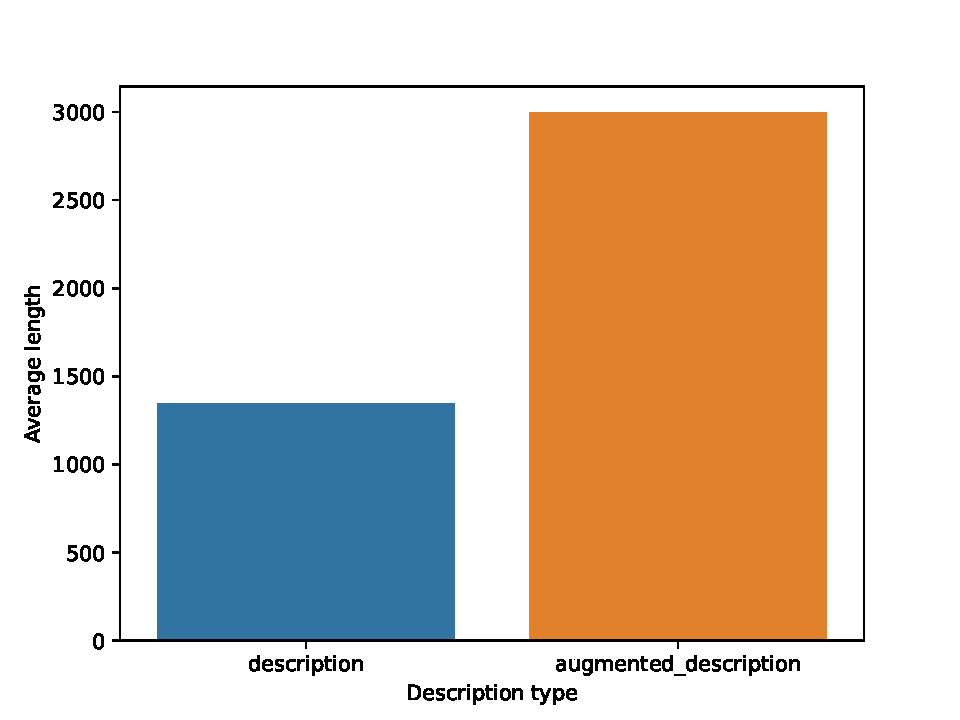
\includegraphics[width=0.65\textwidth]{figures/description_vs_augmented_description.pdf}
    \caption{Histogram of the length of dataset descriptions vs augmented dataset descriptions}
    \label{fig:description_vs_augmented_description}
\end{figure}

\cref{fig:length_of_descriptions} presents a histogram depicting the length of dataset descriptions. The lengths range from 0 to 10,000 words, with the majority of descriptions being under 5,000 words. A few outliers exceed 10,000 words.

\begin{figure}[h]
    \centering
    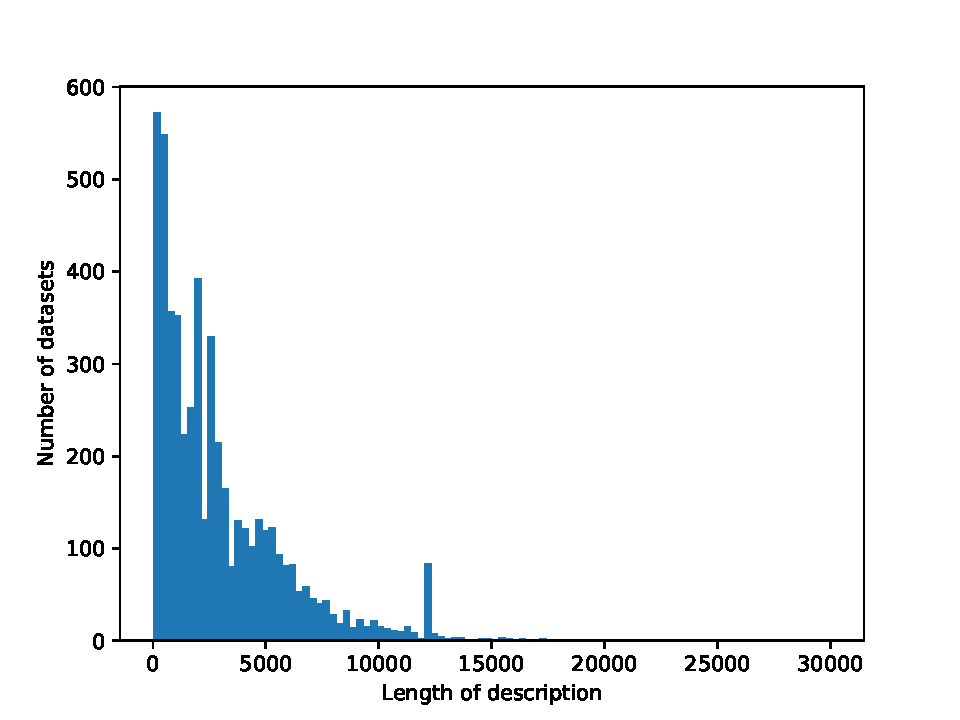
\includegraphics[width=0.85\textwidth]{figures/length_of_descriptions.pdf}
    \caption{Histogram of the length of dataset descriptions}
    \label{fig:length_of_descriptions}
\end{figure}

Similarly, \cref{fig:words_of_descriptions} and \cref{fig:sentences_of_descriptions} display comparable distributions, this time for the number of words and the number of sentences, respectively.

\begin{figure}[h]
    \centering
    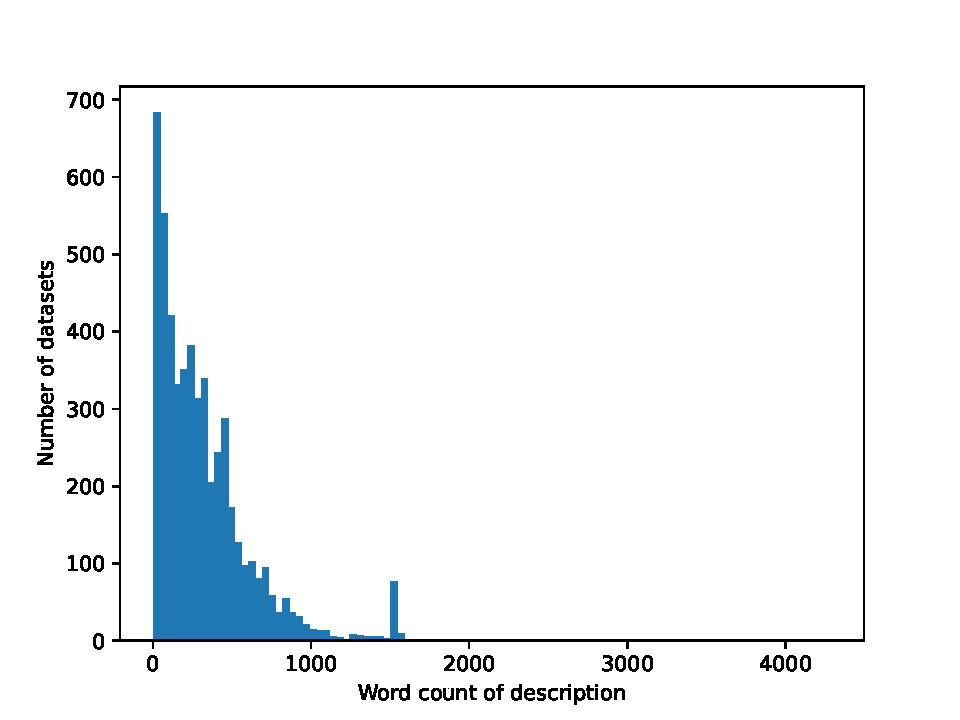
\includegraphics[width=0.85\textwidth]{figures/words_of_descriptions.pdf}
    \caption{Histogram of the number of words of dataset descriptions}
    \label{fig:words_of_descriptions}
\end{figure}

\begin{figure}[h]
    \centering
    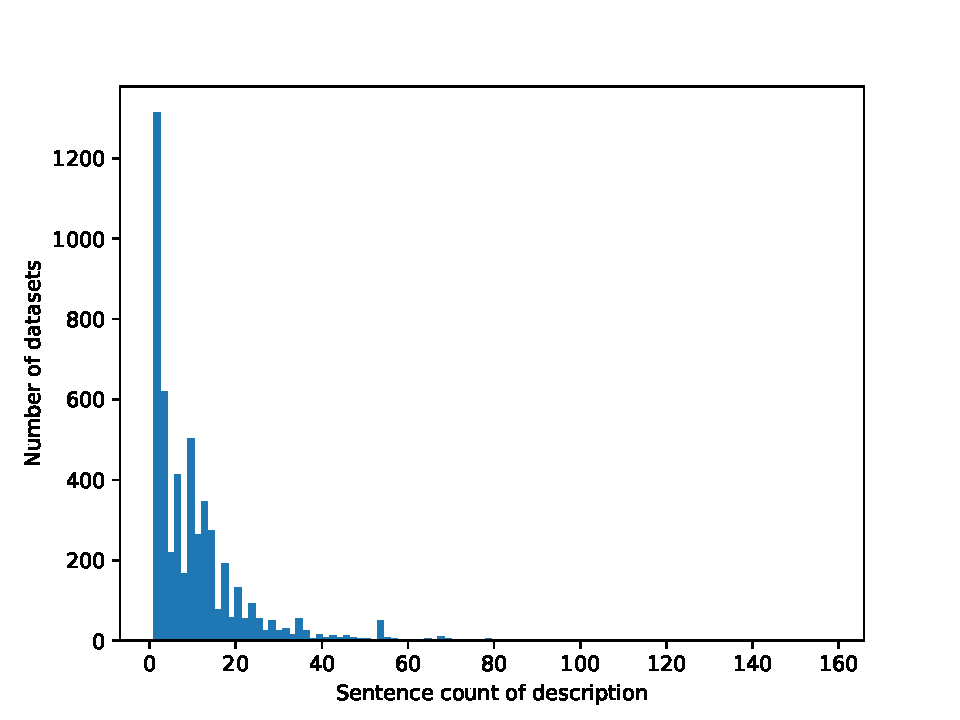
\includegraphics[width=0.85\textwidth]{figures/sentences_of_descriptions.pdf}
    \caption{Histogram of the number of sentences of dataset descriptions}
    \label{fig:sentences_of_descriptions}
\end{figure}

When we examine the availability of tags, we find that the majority of datasets already have tags associated with them (\cref{fig:tag_availability}). This suggests that the tag generation model may be able to leverage the existing tags to improve its performance.

\begin{figure}[h]
    \centering
    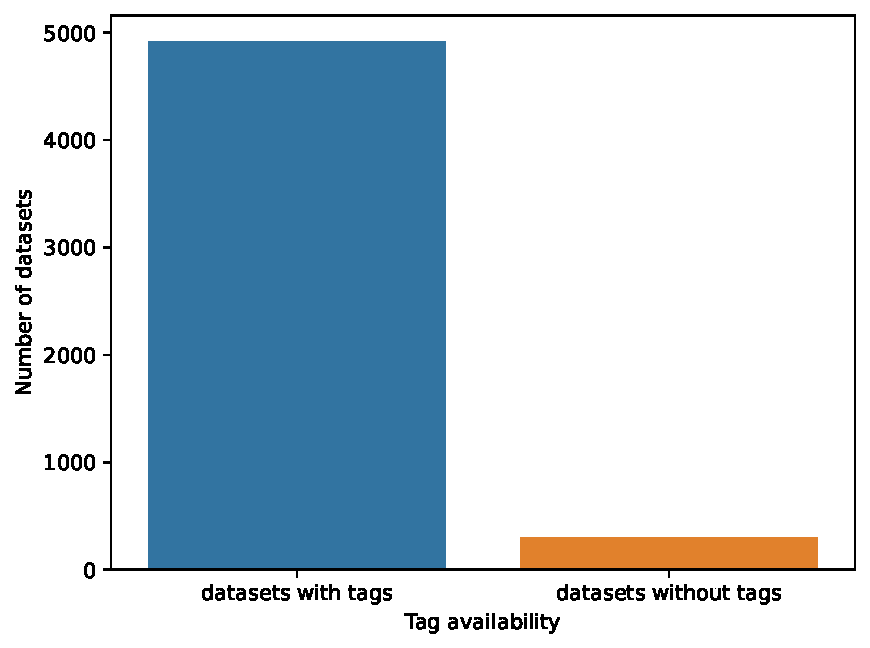
\includegraphics[width=0.85\textwidth]{figures/tag_availability.pdf}
    \caption{Histogram of the number of datasets with and without tags}
    \label{fig:tag_availability}
\end{figure}

When we analyze the number of tags associated with each dataset, we find that most datasets have between 0 and 5 tags, with a few datasets having more than 5 tags (\cref{fig:number_of_tags}).

\begin{figure}[h]
    \centering
    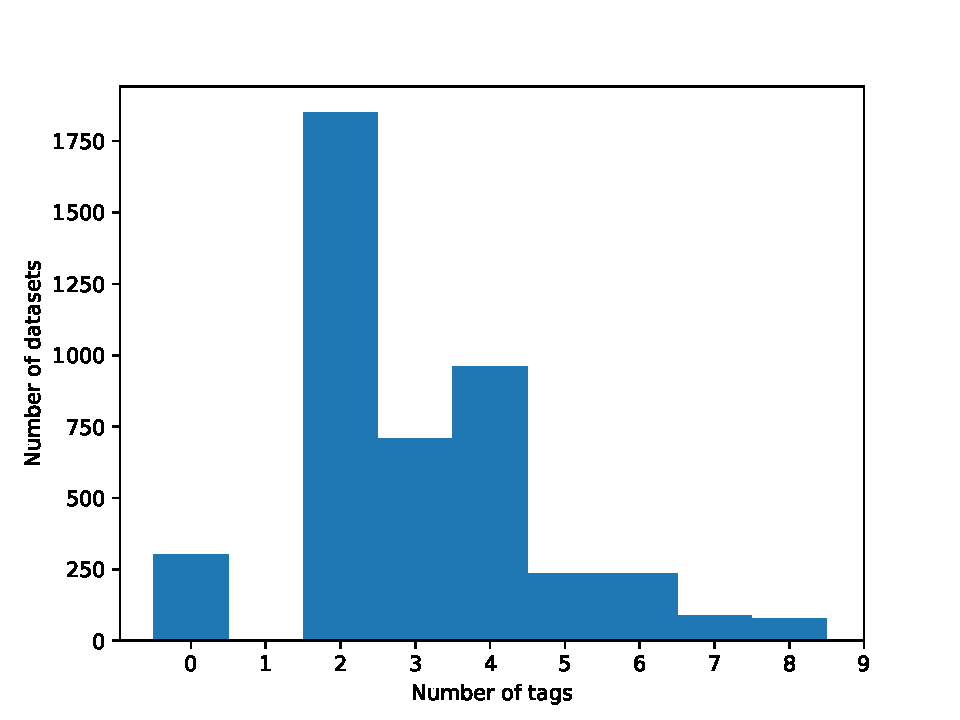
\includegraphics[width=0.85\textwidth]{figures/number_of_tags.pdf}
    \caption{Histogram of the number of tags associated with datasets}
    \label{fig:number_of_tags}
\end{figure}

We then look at the number of features (columns) in the datasets. The distribution of the number of features is shown in \cref{fig:number_of_features}. Most datasets have fewer than 100 features, with a large number of datasets having more than 100 features. This is because those datasets are likely to be high-dimensional datasets from domains such as genomics, text processing, or image analysis, where numerous variables or measurements are collected for each sample.

\begin{figure}[h]
    \centering
    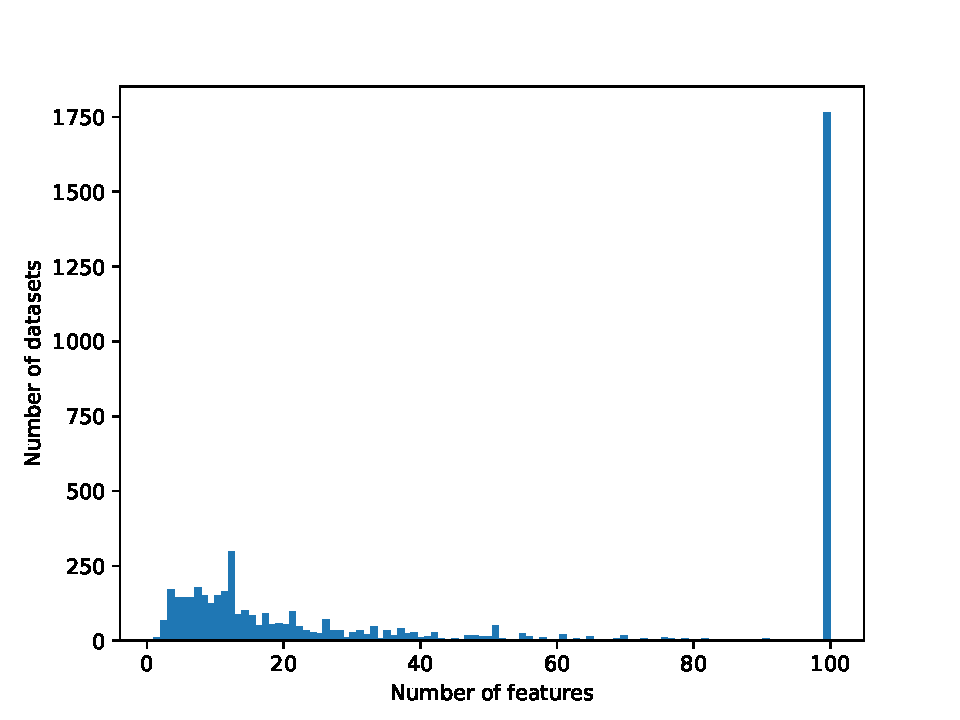
\includegraphics[width=0.7\textwidth]{figures/number_of_features.pdf}
    \caption{Histogram of the number of features in datasets}
    \label{fig:number_of_features}
\end{figure}

Additionally, we examine the cosine similarity between the augmented dataset descriptions to see whether there are datasets with similar descriptions and duplicates. The heatmap of the cosine similarity is shown in \cref{fig:cosine_similarity}. The majority of dataset descriptions have a low cosine similarity, indicating that they are distinct from one another. However, there are some datasets with high cosine similarity, suggesting that they may be duplicates or different versions of the same dataset.

\begin{figure}[h]
    \centering
    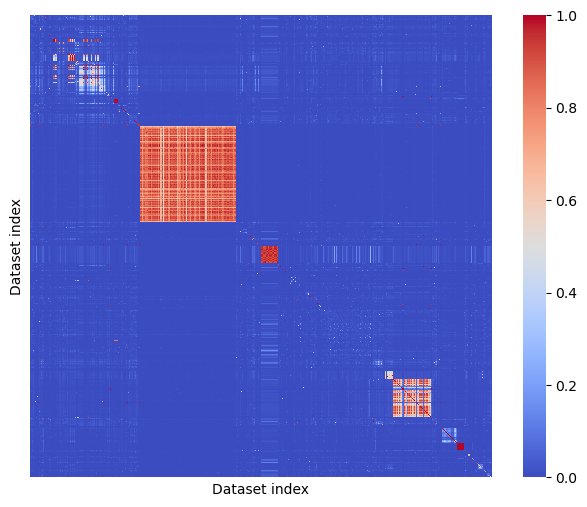
\includegraphics[width=0.85\textwidth]{figures/cosine_similarity.png}
    \caption{Heatmap of the cosine similarity between dataset descriptions}
    \label{fig:cosine_similarity}
\end{figure}

We find that OpenML datasets can have multiple versions. Our analysis of dataset versions reveals that most datasets have only 2 versions, though several datasets have more than 2 (\cref{fig:number_of_versions}).

\begin{figure}[h]
    \centering
    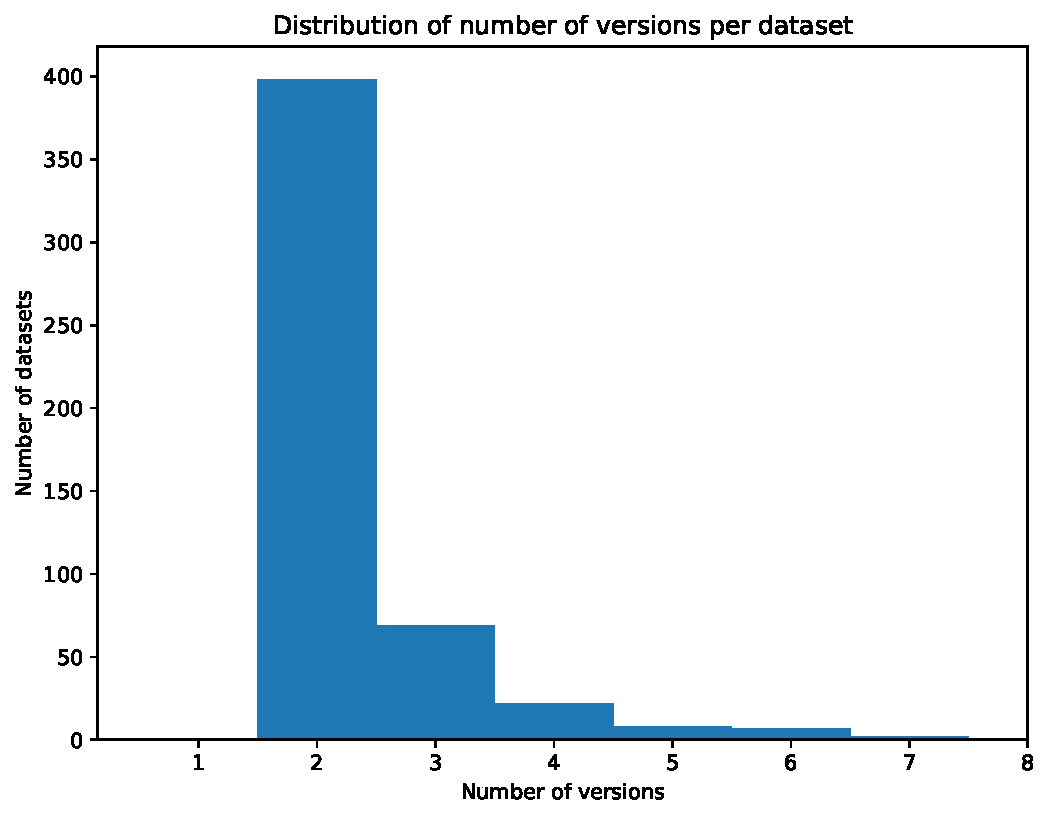
\includegraphics[width=\textwidth]{figures/number_of_versions.pdf}
    \caption{Histogram of the number of versions of dataset descriptions}
    \label{fig:number_of_versions}
\end{figure}

We also examine the similarity between different versions of the datasets. Our analysis shows that most datasets have a cosine similarity of 0.9 or higher within versions, suggesting that the versions are highly similar to one another (\cref{fig:cosine_similarity_dataset_versions}).

\begin{figure}[h]
    \centering
    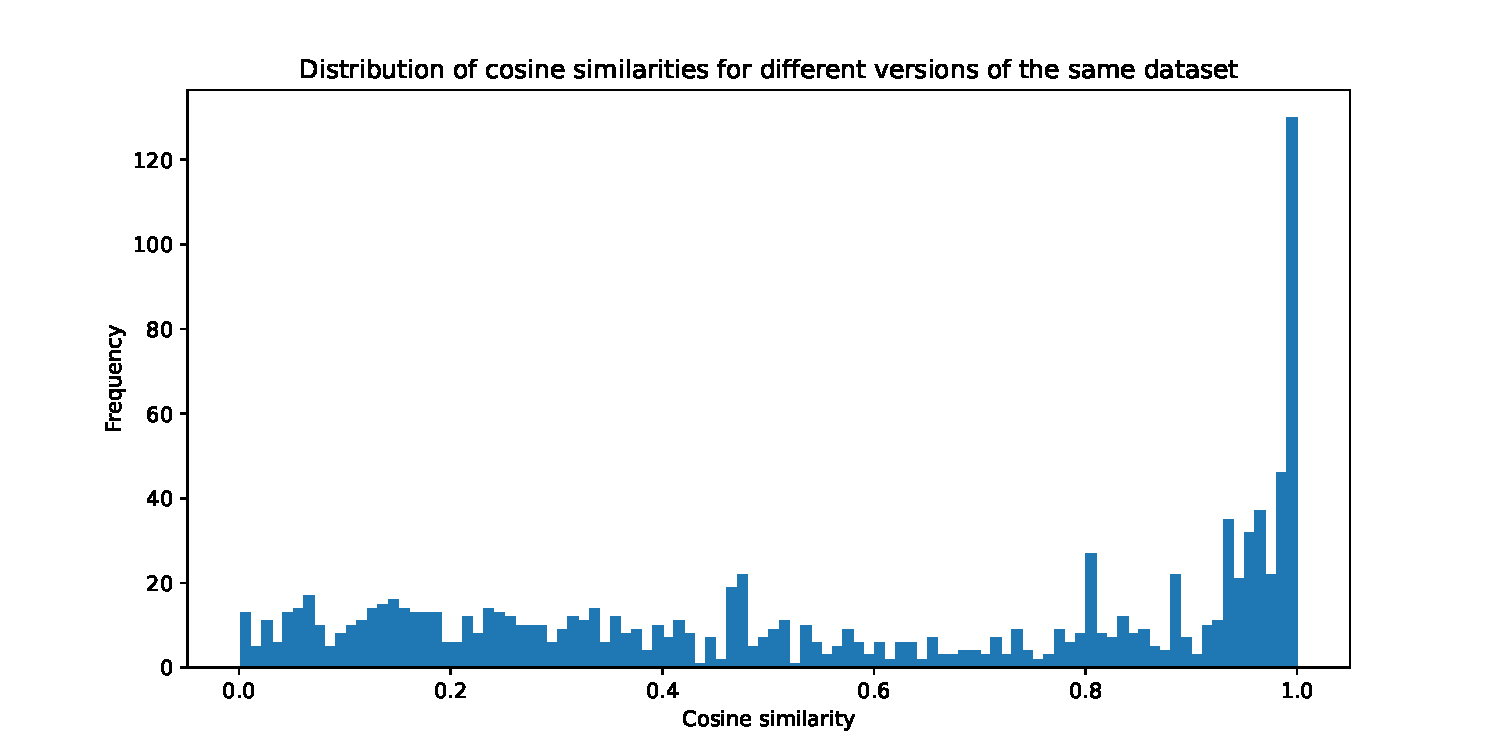
\includegraphics[width=\textwidth]{figures/cosine_similarity_dataset_versions.pdf}
    \caption{Histogram of the cosine similarity of different versions of dataset descriptions}
    \label{fig:cosine_similarity_dataset_versions}
\end{figure}

From these histograms, we can infer that the dataset descriptions are relatively short, with the majority being comparable in length to two Twitter tweets. This is important to note, as descriptions that are too short may lack enough information to generate meaningful tags. However, this may not necessarily pose an issue, as prior studies have successfully applied topic modeling to tweets and other short texts \cite{cataldi_emerging_2010, churchill_percolation-based_2020, curiskis_evaluation_2020, kasiviswanathan_emerging_2011, paul_discovering_2014, yin_dirichlet_2014}.

We apply Named Entity Recognition (NER) and Part-of-Speech (POS) tagging to the dataset descriptions to identify the most common entities and parts of speech (\cref{fig:pos,fig:ner}). A significant number of words are tagged as \textit{X}, indicating that the POS tagger is unable to determine the part of speech for these words. This is likely due to the presence of domain-specific terms not included in the POS tagger's vocabulary, as well as unrecognized or anomalous tokens and symbols. Additionally, we find that the most frequent named entity is \textit{PERSON}, which can be attributed to the fact that many dataset descriptions reference the names of dataset authors or associated papers. Both of these findings pose challenges for the performance of the tag generation model, as unrecognized tokens and author names do not contribute meaningful information for generating relevant tags.

\begin{figure}[h]
    \centering
    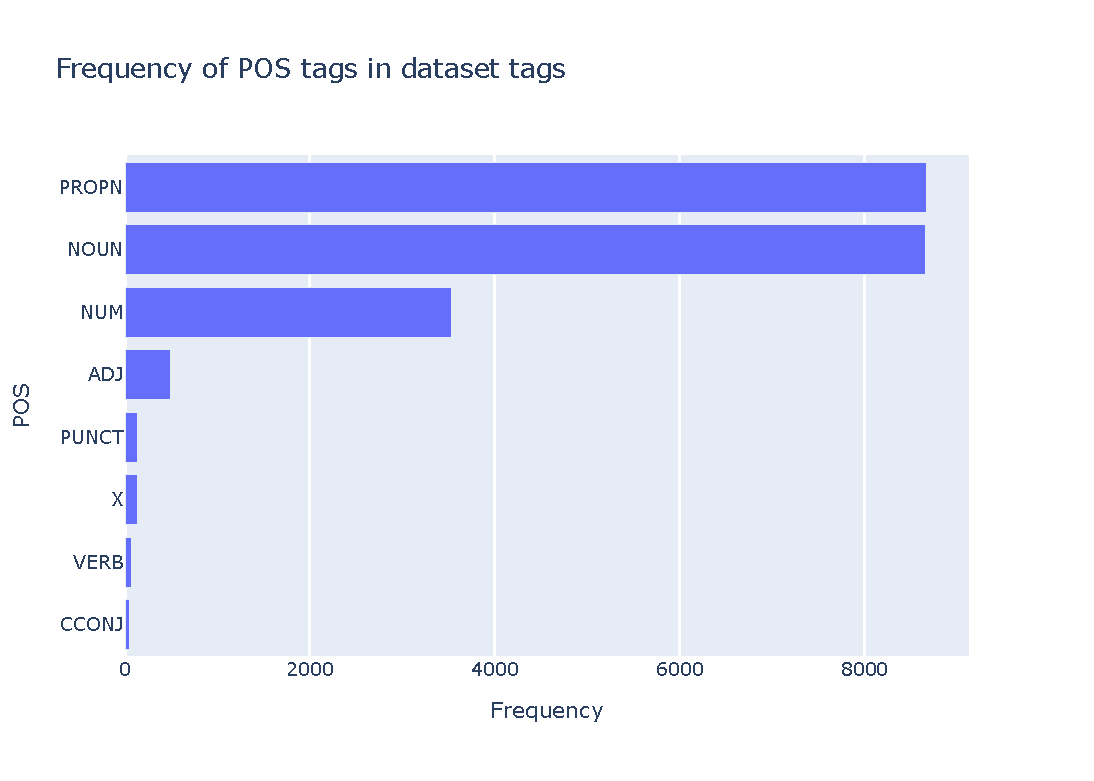
\includegraphics[width=0.9\textwidth]{figures/pos.pdf}
    \caption{Bar chart of the most common parts of speech in dataset descriptions}
    \label{fig:pos}
\end{figure}

\begin{figure}[h]
    \centering
    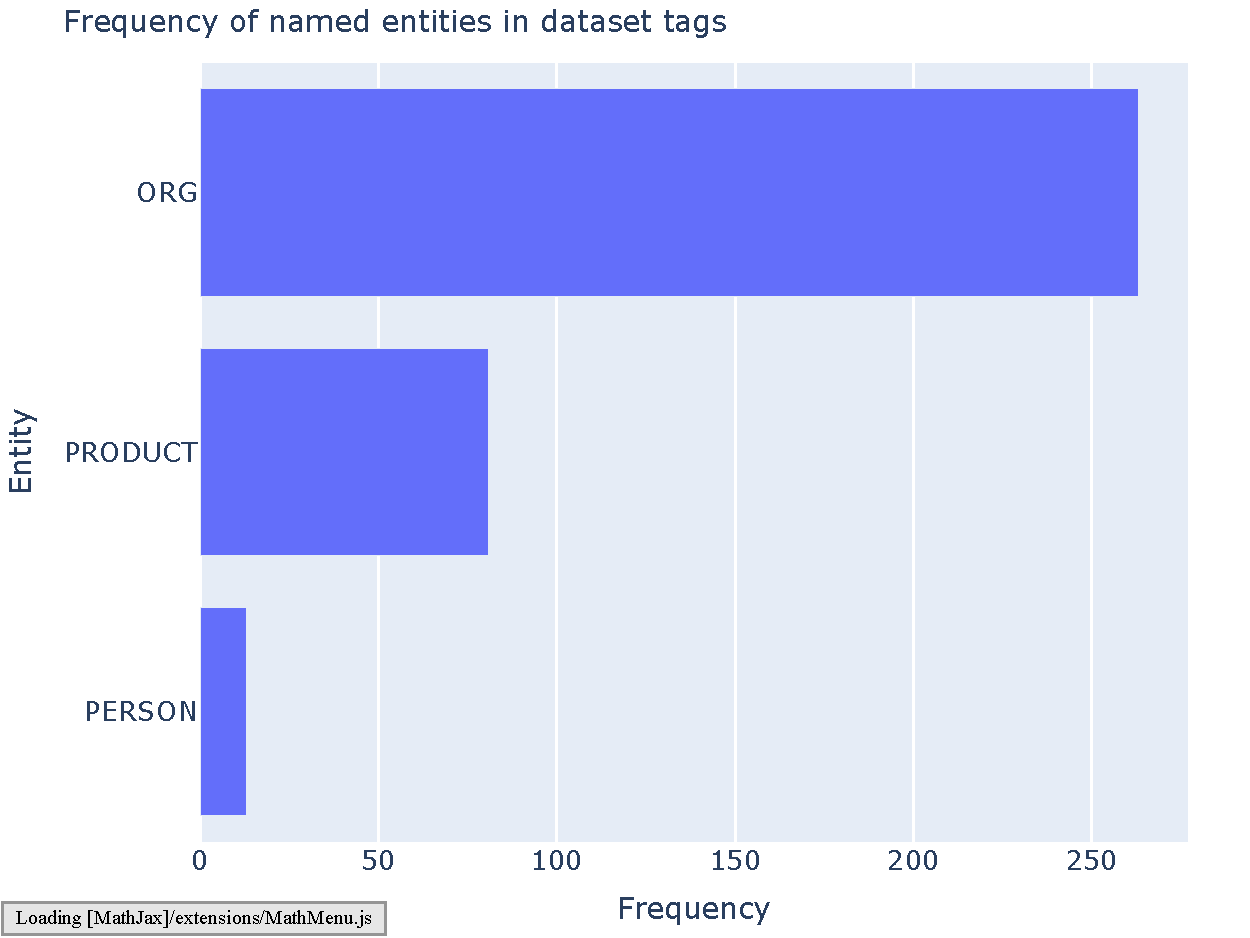
\includegraphics[width=0.9\textwidth]{figures/ner.pdf}
    \caption{Bar chart of the most common named entities in dataset descriptions}
    \label{fig:ner}
\end{figure}

We also examine how many datasets include URLs to original sources in their descriptions (\cref{fig:url_availability}). A significant number of datasets contain URLs, which could be used to scrape additional text for augmenting the descriptions. However, upon closer inspection, we find that the information in these URLs is often redundant with what is already provided in the dataset descriptions. Nonetheless, for some datasets, the URLs contain supplementary information that could be valuable for generating tags, which we scrape.

\begin{figure}[h]
    \centering
    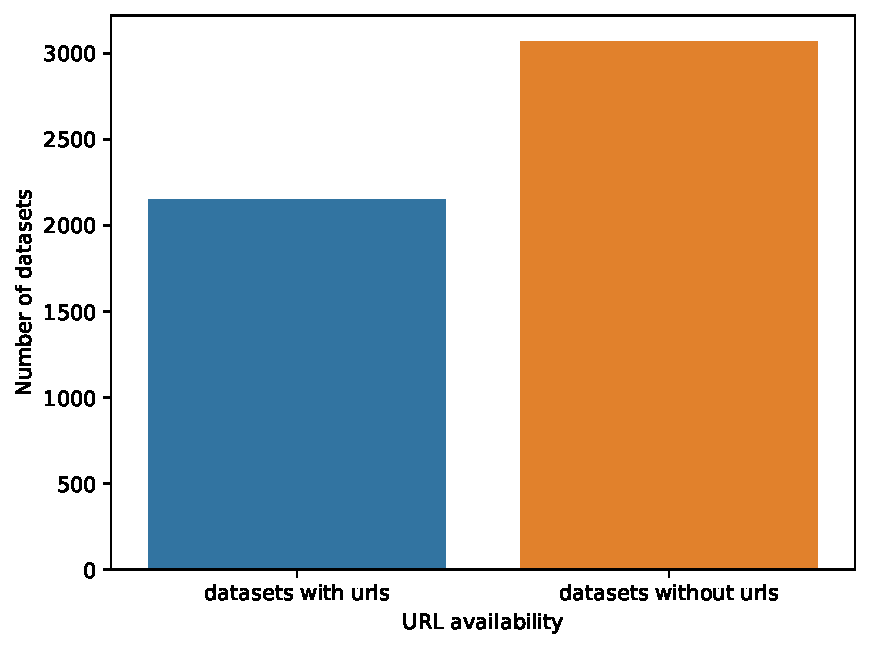
\includegraphics[width=0.85\textwidth]{figures/url_availability.pdf}
    \caption{Bar chart of the number of datasets with and without URLs to original sources}
    \label{fig:url_availability}
\end{figure}

We also explore the readability and complexity of the dataset descriptions by calculating the Flesch Reading Ease \cite{flesch_new_1948} (\cref{fig:flesch_reading_ease}). The Flesch Reading Ease score ranges from 0 to 100, with higher scores indicating easier readability. We find that the dataset descriptions are somewhat difficult to read, with many falling in the 0-60 range. This suggests that the descriptions may contain complex language and jargon that could require specialized knowledge to understand. This may also affect the embedding model performance, as it may struggle to capture the semantic meaning of complex or domain-specific terms which the embedding model has not been trained on.

\begin{figure}[h]
    \centering
    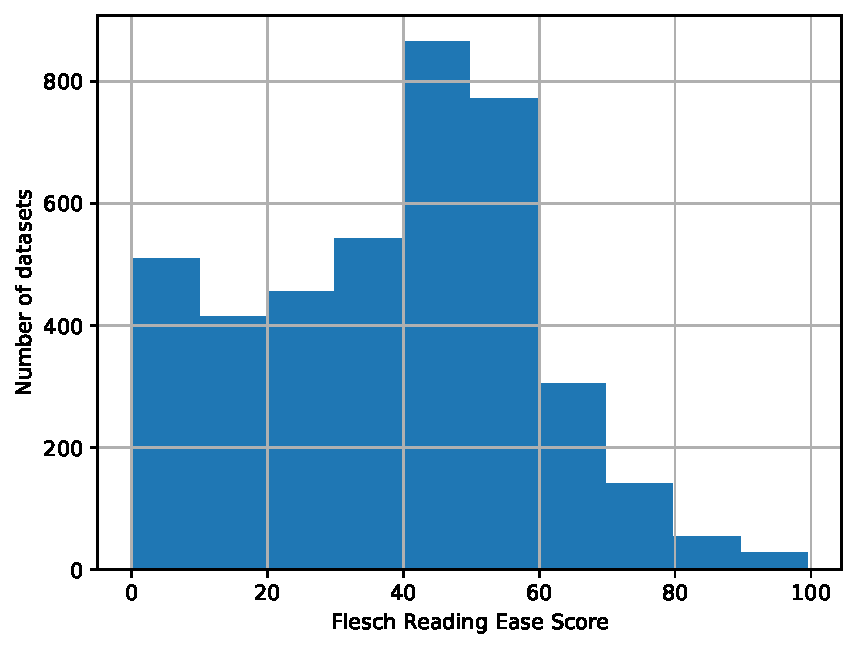
\includegraphics[width=0.85\textwidth]{figures/flesch_reading_ease.pdf}
    \caption{Bar chart of the number of datasets with and without URLs to original sources}
    \label{fig:flesch_reading_ease}
\end{figure}

In this section, we described the most pertinent findings from our data exploration. For readers interested in a more detailed analysis, additional information can be found in the \textit{eda.ipynb} notebook in the \href{https://github.com/ivangermanov/openml-tags}{GitHub repository} \cite{germanov_topic_modeling_of_2024}.

\section{Automated evaluation metrics and baselines}
We first explain the hyperparameter tuning (Bayesian optimization) process. Then, we explain the baseline models we use and what parameters we choose for them. We showcase the results of the comparison between the baseline models and the hyperparameter-optimized BERTopic model.

\subsection{Hyperparameter tuning}
Using OCTIS, we perform hyperparameter tuning for the \textit{Base BERTopic model}. As an objective metric, we use the weighted metric we defined in \cref{sec:hyperparameter_tuning}. We set ranges for the hyperparameters, which are based on prior knowledge of good default values and the OpenML dataset characteristics. The hyperparameters and their respective search spaces are as follows:

\begin{itemize}
    \item \textbf{min\_topic\_size}: This determines the minimum number of documents a topic should have. We set the range to [2, 3] to explore small topic sizes.
    \item \textbf{ctfidf\_reduce\_frequent\_words}: This boolean hyperparameter determines whether frequent words should be reduced when constructing the c-TF-IDF matrix. The values considered are \texttt{True} or \texttt{False}.
    \item \textbf{umap\_n\_neighbors}: This hyperparameter controls the number of neighbors considered in the UMAP algorithm. We set the range to [2, 3]. We choose smaller values, since larger values result in more global views of the manifold, while smaller values result in more local data being preserved.
    \item \textbf{umap\_n\_components}: This controls the number of dimensions UMAP reduces the embeddings to. We have set the range to [2, 10].
    \item \textbf{umap\_min\_dist}: This defines the minimum distance between points in the UMAP embedding space. We are exploring a small range of [0.0, 0.01].
    \item \textbf{umap\_metric}: The metric used to calculate distances between points in the UMAP algorithm. The two metrics we consider are 'cosine' and 'euclidean'.
    \item \textbf{hdbscan\_min\_cluster\_size}: This defines the minimum cluster size for HDBSCAN. We set the range to [2, 3]. Similarly to \texttt{min\_topic\_size} and \texttt{umap\_n\_neighbors}, we explore small values to capture smaller clusters.
    \item \textbf{hdbscan\_metric}: This defines the distance metric used by HDBSCAN. We restrict this to 'euclidean'.
    \item \textbf{hdbscan\_cluster\_selection\_method}: This determines how clusters are selected in HDBSCAN. We use \textit{eom} (excess of mass).
    \item \textbf{vectorizer\_ngram\_range}: This defines the n-gram range for the vectorizer. We consider both unigram (1,1) and bigram (1,2) settings.
    \item \textbf{vectorizer\_stop\_words}: We set the stop words for vectorization to be 'english'.
    \item \textbf{vectorizer\_tokenizer}: This boolean hyperparameter controls whether a custom tokenizer is used. We set this to \texttt{False}.
    \item \textbf{outliers\_strategy}: This defines how outliers should be handled. For this study, we set it to \textit{none}, meaning that no specific outlier handling strategy is applied.
    \item \textbf{embedding\_model}: This hyperparameter defines the embedding model used for the \textit{Base BERTopic model}. Since they are slower to evaluate, we only consider the \texttt{Salesforce/\allowbreak SFR-Embedding-\allowbreak Mistral} model, as it was SOTA on the MTEB leaderboard at the time of writing.
    \item \textbf{representation\_model}: This hyperparameter defines the representation model used for the BERTopic model. Since they are slower to evaluate, we only consider spaCy's Part-of-Speech model called \texttt{en\_core\_web\_lg}.
\end{itemize}

This automated hyperparameter optimization process allows us to systematically explore the space of possible configurations and identify the best-performing model for our dataset.

As for the Bayesian optimization \cite{archetti_bayesian_2019, galuzzi_hyperparameter_2020, snoek_practical_2012}, we employ the \texttt{Optimizer} class from OCTIS. This method efficiently explores the hyperparameter space by constructing a probabilistic (surrogate) model to approximate the objective function. In our case, the surrogate model is a Random Forest (RF), which is updated iteratively to predict the performance of unobserved hyperparameter configurations based on previous evaluations.

The surrogate model relies on the Matern kernel with a smoothness parameter \( \nu = 1.5 \). This kernel helps balance the trade-off between exploration and exploitation by controlling the smoothness of the Gaussian process used in the optimization.

To guide the search for optimal hyperparameters, we use the Lower Confidence Bound (LCB) acquisition function. The LCB acquisition function is particularly effective in encouraging exploration of uncertain regions while still exploiting areas that show high potential for improvement.

Before the optimization begins, we initialize the surrogate model with a diverse set of hyperparameter configurations. These initial points are generated using Latin Hypercube Sampling (LHS), which ensures a broad coverage of the search space from the outset.

Additionally, we set the number of iterations for the optimization process to 125, and the number of model runs per iteration to 3. This configuration allows us to explore the hyperparameter space thoroughly while maintaining a reasonable computational cost. We set the model runs to 3 to account for the stochastic nature of the BERTopic model (specifically, UMAP), which can yield slightly different results for each run.

\cref{fig:bayesian_optimization} shows the results of the Bayesian optimization process. The x-axis represents the number of iterations, while the y-axis represents the weighted metric score, \textit{Median(model\_runs)} and \textit{Mean(model\_runs)}, and other metrics. We can see that the optimization process converges to a stable solution relatively quickly. This indicates that the hyperparameter search space has been thoroughly explored, and a good configuration has been found. We also observe that there are many hyperparameter configurations that perform similarly. This suggests that the BERTopic model is robust to changes in hyperparameters and can achieve good performance across a wide range of settings.

\begin{figure}[h]
    \centering
    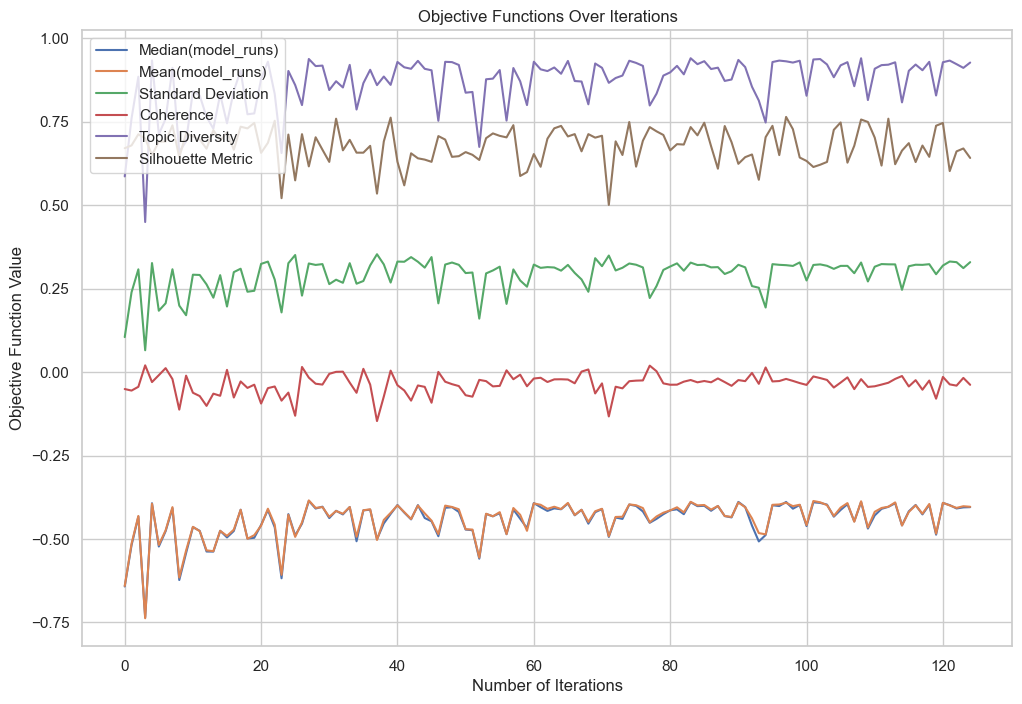
\includegraphics[width=0.8\textwidth]{figures/bayesian_optimization.png}
    \caption{Results of the Bayesian optimization process}
    \label{fig:bayesian_optimization}
\end{figure}

\subsection{Baselines}
\subsubsection{Definition of Baselines}
We select the hyperparameter-optimized BERTopic model as our primary model and compare its performance against several baseline models. The baseline models are as follows:
\begin{enumerate}
    \item \textbf{BERTopic model with default parameters}: This model uses the default hyperparameters provided by the BERTopic library. We use this model to compare the performance of the hyperparameter-optimized model with the default settings.
    \item \textbf{LDA}: We fit an LDA model to the dataset descriptions using the \texttt{LDA} class from OCTIS. LDA is a model which requires cleaning and preprocessing of the text data, such as removing stop words, stemming, and lemmatization. We use the default settings for the LDA model.
    \item \textbf{NMF}: We fit an NMF model to the dataset descriptions using the \texttt{NMF} class from OCTIS. We use the default settings for the NMF model.
    \item \textbf{CTM}: We fit a CTM model to the dataset descriptions using the \texttt{CTM} class from the Contextualized Topic Models library \cite{noauthor_milanlproccontextualized-topic-models_2024}. We preprocess the data and create the required embeddings with the \texttt{all-mpnet-base-v2} embedding model and use the default settings for the CTM model with the \texttt{contextual\_size} parameter set to 768.
    \item \textbf{Top2Vec}: We fit a custom implementation of Top2Vec based on the original model. This implementation uses the \texttt{all-mpnet-base-v2} embedding model from the Sentence Transformers library for document and word embeddings. The HDBSCAN clustering algorithm is used with custom arguments set in the \texttt{hdbscan\_args} parameter. We use the \texttt{Top2VecNew} class from our custom implementation, which allows for more flexibility in topic number specification.
\end{enumerate}

For each model, we train using a predefined set of topic numbers. This approach is necessary because some models require a fixed number of topics, while others, such as BERTopic, can either operate with a fixed number or determine the number of topics automatically. Specifically, we set the number of topics to 10, 20, 30, 40, 50, 100, and 200.

Additionally, for each specified number of topics, we run each model 10 times to account for their stochastic nature. This approach allows us to later assess whether there are statistically significant differences in the models' performance.

\subsubsection{Results}
In \cref{fig:openml_npmi} we present the NPMI scores for the hyperparameter-optimized BERTopic model and the baseline models. The NPMI score is a measure of topic coherence, with higher scores indicating more coherent topics. There are several BERTopic models with different hyperparameters:
\begin{itemize}
    \item \textbf{BERTopic\_optimized\_POS\_reduced\_range}: The BERTopic model we optimized with Bayesian optimization above.
    \item \textbf{BERTopic\_optimized\_POS\_full\_range}: Similar to the previous model, but with a wider range of hyperparameters. We choose not to use this model as we are interested in exploring smaller topic sizes, but we provide it for comparison.
    \item \textbf{BERTopic\_POS}: The BERTopic model with default hyperparameters (also with the spaCy Part-of-Speech model as the representation model).
    \item \textbf{BERTopic\_POS\_mpnet}: Similar to the previous model, but with the \texttt{all-mpnet-base-v2} embedding model instead of \texttt{Salesforce/SFR-Embedding-Mistral}.
\end{itemize}

\begin{figure}[h]
    \centering
    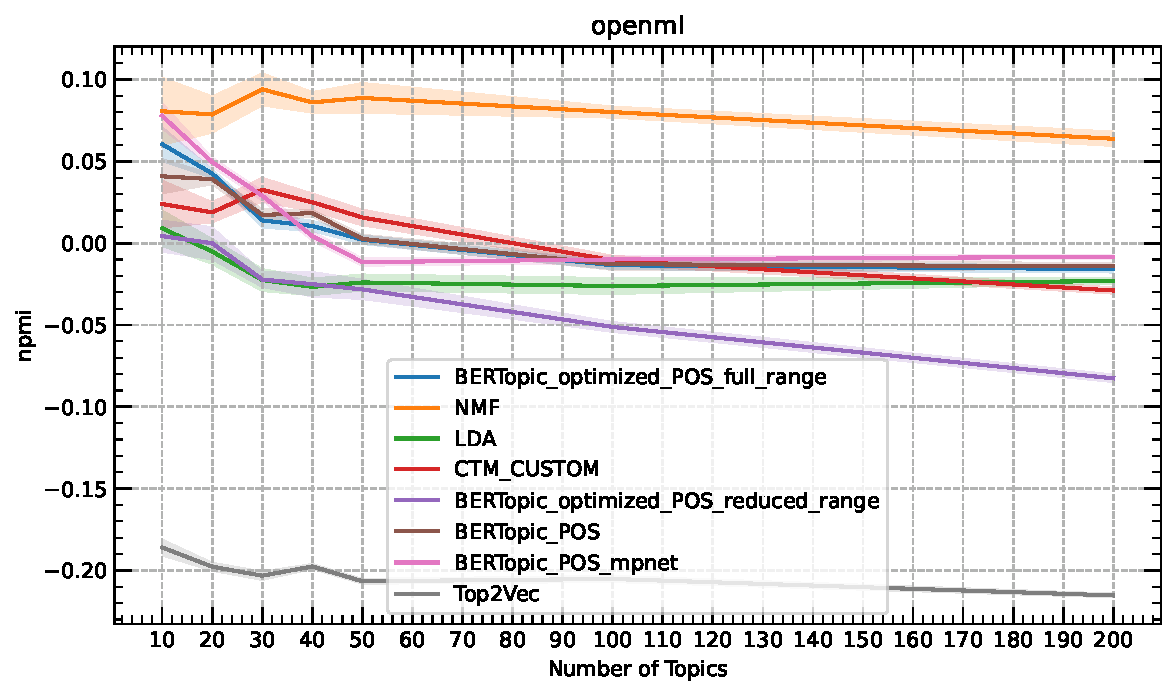
\includegraphics[width=0.85\textwidth]{figures/openml_npmi.pdf}
    \caption{Line chart of the NPMI scores for the hyperparameter-optimized BERTopic model and the baseline models}
    \label{fig:openml_npmi}
\end{figure}

We observe that the NMF model outperforms all models across all topic numbers. However, when we look at \cref{fig:openml_diversity}, we see that the NMF model has very low diversity scores. This suggests that the NMF model may be picking the same terms in each topic, leading to high coherence but low diversity. For NPMI, we then see that the BERTopic models perform the second best, with very small differences between them. We see that \textbf{BERTopic\_optimized\_POS\_reduced\_range} performs slightly worse, but this is likely due to the smaller topic sizes we explored. We see that LDA, CTM, and Top2Vec perform worse than the BERTopic models.

As for diversity, we see that the \textbf{BERTopic\_optimized\_POS\_reduced\_range} has the highest average diversity scores, followed by the other BERTopic models. This suggests that the BERTopic models are able to capture a wider range of terms in their topics compared to the other models. Surprisingly, the Top2Vec model has the lowest NPMI and diversity scores.

\begin{figure}[h]
    \centering
    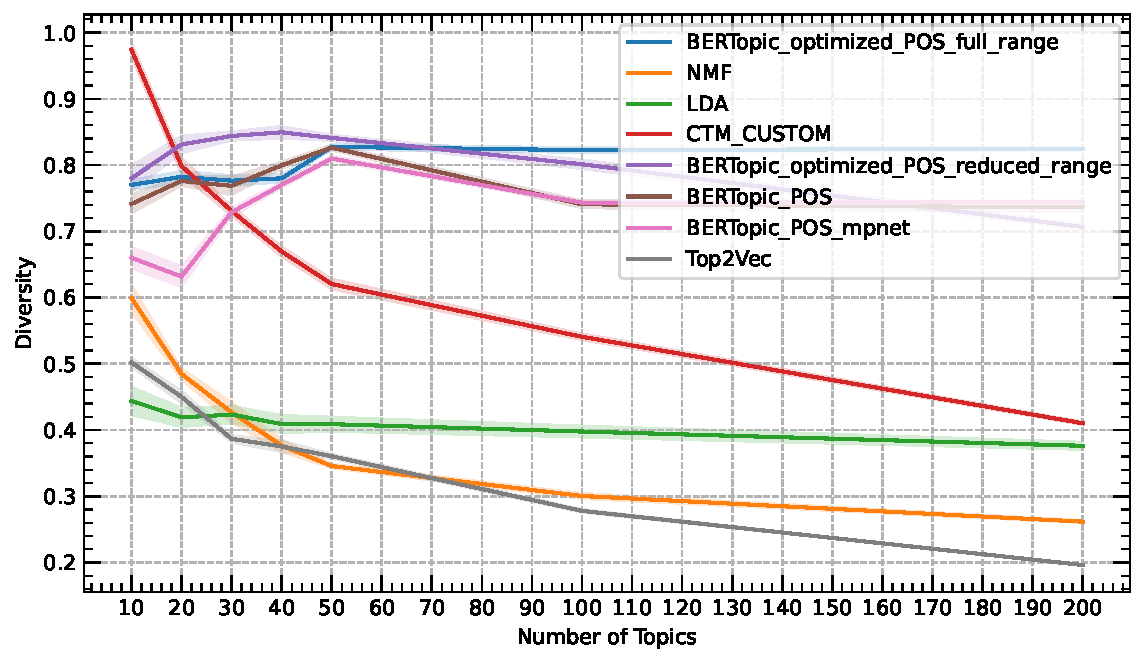
\includegraphics[width=0.85\textwidth]{figures/openml_diversity.pdf}
    \caption{Line chart of the diversity scores for the hyperparameter-optimized BERTopic model and the baseline models}
    \label{fig:openml_diversity}
\end{figure}

In \cref{tab:openml_results}, we present the NPMI and diversity scores for the models. We highlight the best scores in dark green and the subsequent best scores in lighter green. We see that the BERTopic models perform well in terms of diversity, with the \textbf{BERTopic\_optimized\_POS\_reduced\_range} model having the highest diversity score. If we only look at the BERTopic models, we can note a strong negative Pearson correlation between NPMI and diversity scores of -0.67. This suggests that the higher coherence may be driven by the inclusion of more common terms in the topics, while the diversity score is driven by the inclusion of more unique terms. In any case, the BERTopic models outperform the baseline models in terms of combined NPMI and diversity scores.

\begin{table}[h]
    \centering
    \definecolor{color64db00}{HTML}{64db00}
    \definecolor{color76FF03}{HTML}{76FF03}
    \definecolor{colore1ffc7}{HTML}{e1ffc7}
    \begin{tabular}{>{\centering\arraybackslash}m{25em}>{\centering\arraybackslash}m{7em}>{\centering\arraybackslash}m{7em}}
        \toprule
        \textbf{Model}                           & \textbf{npmi}                 & \textbf{diversity}            \\
        \midrule
        Top2Vec                                  & -0.202                        & 0.364                         \\
        BERTopic\_optimized\_POS\_reduced\_range & -0.029                        & \cellcolor{color64db00} 0.808 \\
        LDA                                      & -0.017                        & 0.411                         \\
        CTM\_CUSTOM                              & 0.011                         & 0.678                         \\
        BERTopic\_POS                            & 0.013                         & \cellcolor{colore1ffc7} 0.770 \\
        BERTopic\_optimized\_POS\_full\_range    & \cellcolor{colore1ffc7} 0.014 & \cellcolor{color76FF03} 0.798 \\
        BERTopic\_POS\_mpnet                     & \cellcolor{color76FF03} 0.019 & 0.727                         \\
        NMF                                      & \cellcolor{color64db00} 0.082 & 0.399                         \\
        \bottomrule
    \end{tabular}
    \caption{NPMI and diversity scores for the hyperparameter-optimized BERTopic model and the baseline models}
    \label{tab:openml_results}
\end{table}

\subsubsection{Statistical significance}
As mentioned earlier, we had 10 runs for each model and topic number combination. We will now assess whether there are statistically significant differences between the performance of the models. We check whether the assumptions for ANOVA are met, and if not, we use Welch's ANOVA or Kruskal-Wallis (non-parametric) tests.

The first assumption for ANOVA is that the residuals are normally distributed. We apply the Shapiro-Wilk test to check whether the residuals for the NPMI values (the differences between the observed and predicted NPMI values) are normally distributed. The Shapiro-Wilk test returned a statistic of 0.905 and a p-value of 3.30e-18, indicating a significant deviation from normality. Although the statistic is relatively close to 1, suggesting that the residuals are not drastically non-normal, the extremely small p-value suggests that the deviation is statistically significant. As for the diversity values, the Shapiro-Wilk test returned a statistic of 0.968 and a p-value of 8.70e-10, also indicating a significant deviation from normality, but with a statistic even closer to 1.

Given this result, we further inspect the residuals using visual diagnostics with Q-Q plots and histograms to assess the nature and extent of the deviation from normality. If the deviation is minor, ANOVA may still be appropriate. \cref{fig:qqplot_npmi} and \cref{fig:histogram_npmi} show the Q-Q plot and histogram of the residuals for the NPMI values, respectively. We observe that the residuals are approximately normally distributed, with some deviations at the tails. \cref{fig:qqplot_diversity} and \cref{fig:histogram_diversity} show the Q-Q plot and histogram of the residuals for the diversity values, respectively. We observe a similar pattern for the diversity residuals, with some deviations at the tails. Given that ANOVA is relatively robust to deviations at the tails, since extreme values do not have a large impact on the F-statistic, we consider this assumption to be met.

\begin{figure}[h]
    \centering
    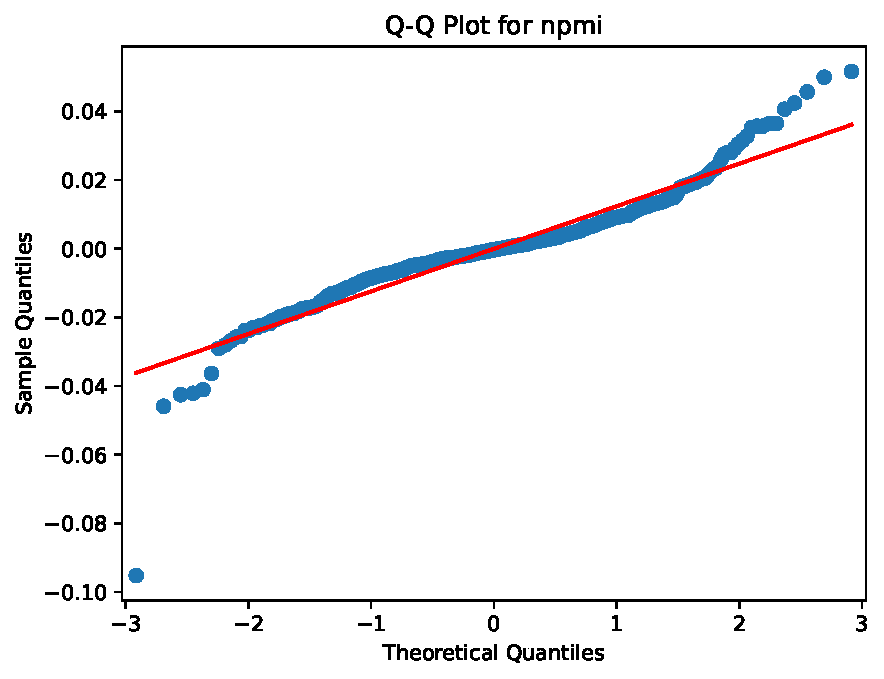
\includegraphics[width=0.85\textwidth]{figures/qqplot_npmi.pdf}
    \caption{Q-Q plot of the residuals for the NPMI values}
    \label{fig:qqplot_npmi}
\end{figure}

\begin{figure}[h]
    \centering
    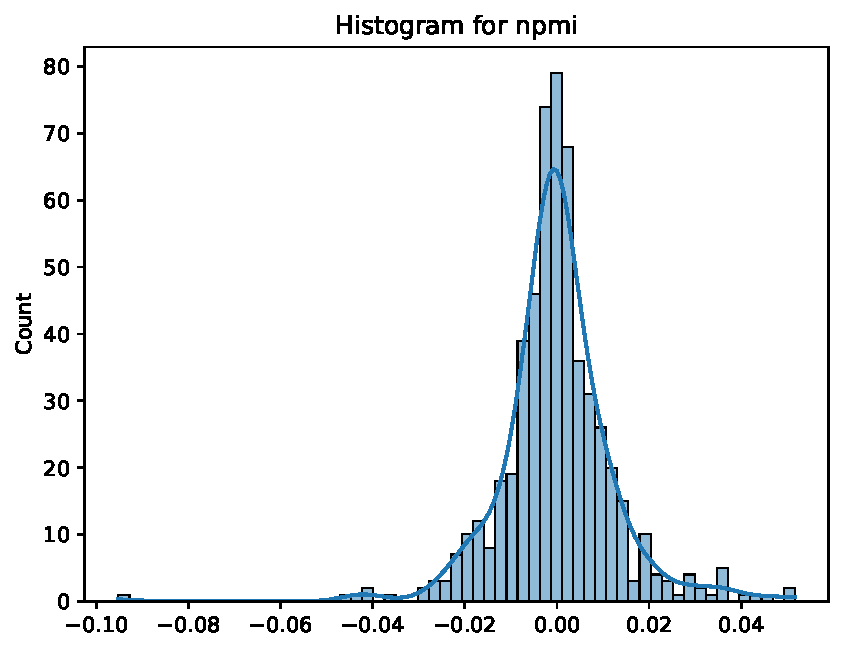
\includegraphics[width=0.85\textwidth]{figures/histogram_npmi.pdf}
    \caption{Histogram of the residuals for the NPMI values}
    \label{fig:histogram_npmi}
\end{figure}

\begin{figure}[h]
    \centering
    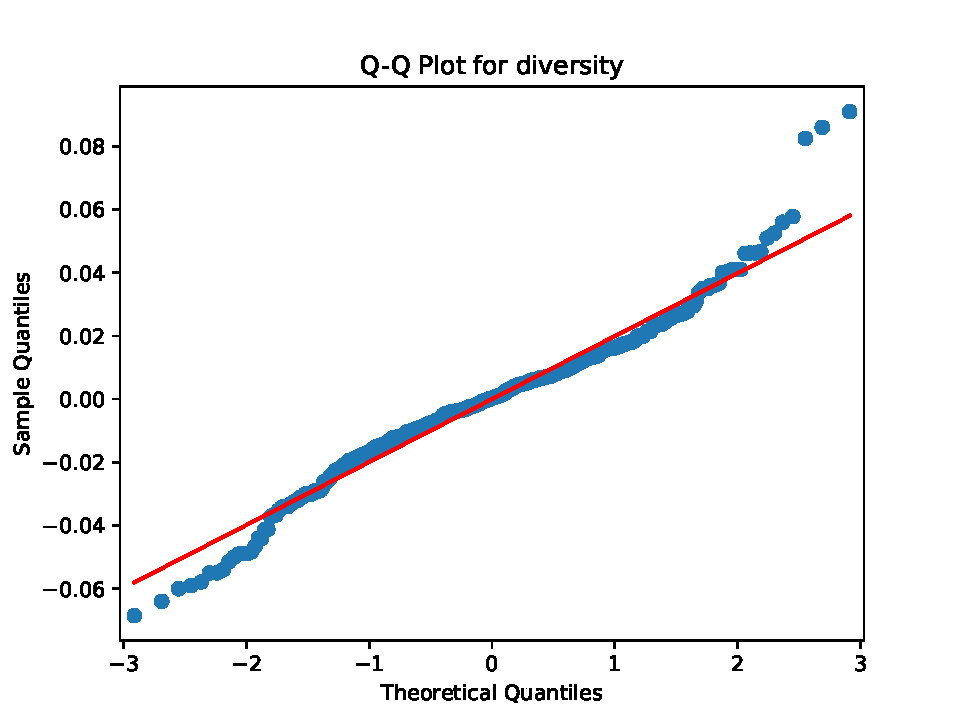
\includegraphics[width=0.85\textwidth]{figures/qqplot_diversity.pdf}
    \caption{Q-Q plot of the residuals for the diversity values}
    \label{fig:qqplot_diversity}
\end{figure}

\begin{figure}[h]
    \centering
    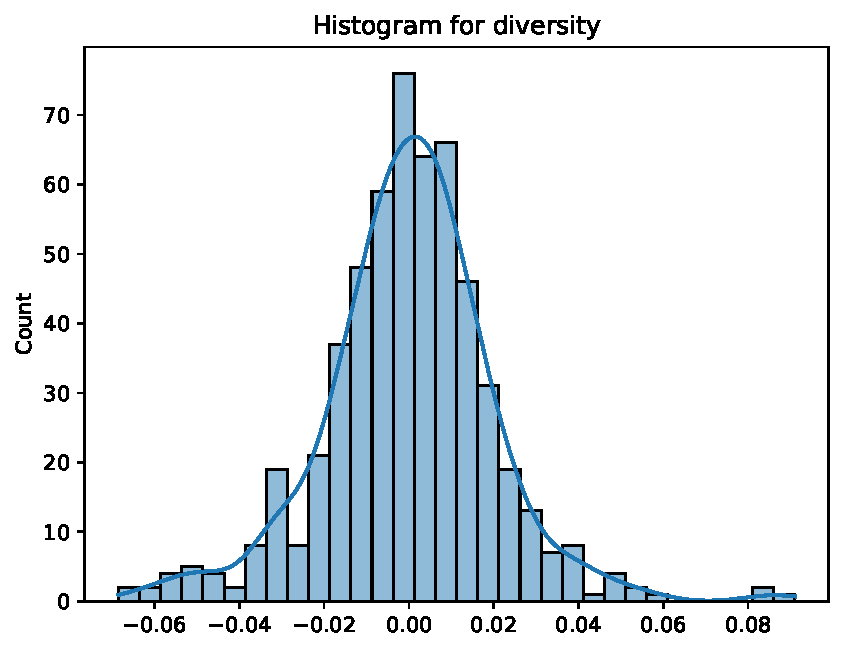
\includegraphics[width=0.85\textwidth]{figures/histogram_diversity.pdf}
    \caption{Histogram of the residuals for the diversity values}
    \label{fig:histogram_diversity}
\end{figure}

The second assumption for ANOVA is that the residuals have equal variance. We apply the Levene test and the Bartlett test to check whether the residuals have equal variance, for each model and topic number combination. \cref{tab:levene_bartlett} shows the results of the Levene and Bartlett tests for the NPMI and diversity values. We observe that the p-values are mostly below 0.05, indicating that the residuals do not have equal variance. This violates the assumption of homoscedasticity (equal variance) for ANOVA. Therefore, we will use Welch's ANOVA, since the first assumption is met, and the residuals are approximately normally distributed, but the assumption of equal variance is violated.

\begin{table}[htbp]
    \centering
    \caption{Levene's and Bartlett's tests for NPMI and diversity}
    \begin{tabular}{@{}lcc|cc@{}}
        \toprule
                            & \multicolumn{2}{c}{\textbf{NPMI}} & \multicolumn{2}{c}{\textbf{Diversity}}                                         \\ \cmidrule(lr){2-3} \cmidrule(lr){4-5}
        \textbf{nr\_topics} & \textbf{Statistic}                & \textbf{p-value}                       & \textbf{Statistic} & \textbf{p-value} \\ \midrule
        \multicolumn{5}{c}{\textbf{Levene's Test}}                                                                                               \\ \midrule
        10                  & 1.4665                            & 0.1930                                 & 1.6530             & 0.1346           \\
        20                  & 4.0018                            & 0.0009                                 & 1.2666             & 0.2791           \\
        30                  & 2.9904                            & 0.0082                                 & 2.0219             & 0.0638           \\
        40                  & 2.6662                            & 0.0164                                 & 1.1821             & 0.3239           \\
        50                  & 2.9896                            & 0.0082                                 & 2.5184             & 0.0225           \\
        100                 & 1.0988                            & 0.3733                                 & 1.4504             & 0.1990           \\
        200                 & 2.4367                            & 0.0268                                 & 2.6070             & 0.0186           \\ \midrule
        \multicolumn{5}{c}{\textbf{Bartlett's Test}}                                                                                             \\ \midrule
        10                  & 19.3408                           & 0.0072                                 & 17.4000            & 0.0150           \\
        20                  & 39.6442                           & 1.4724e-06                             & 7.5180             & 0.3770           \\
        30                  & 24.0258                           & 0.0011                                 & 14.8213            & 0.0384           \\
        40                  & 27.6841                           & 0.0003                                 & 11.7576            & 0.1088           \\
        50                  & 34.6455                           & 1.3038e-05                             & 19.0298            & 0.0081           \\
        100                 & 9.8099                            & 0.1996                                 & 15.5252            & 0.0298           \\
        200                 & 20.3993                           & 0.0048                                 & 31.0744            & 6.0240e-05       \\ \bottomrule
    \end{tabular}
    \label{tab:levene_bartlett}
\end{table}

Applying Welch's ANOVA to the NPMI and diversity values, we find that there are statistically significant differences between the models for both metrics (\cref{tab:welch_anova}). For NPMI, 90.75\% of the variance is explained by the model, and for diversity, 81.50\% of the variance is explained by the model. These are both large effect sizes, suggesting that the models have a substantial impact on both metrics.

We then perform post-hoc tests to determine which models are significantly different from one another. We use the Games-Howell post-hoc test, which is appropriate when the assumption of equal variance is violated. The results of the Games-Howell post-hoc test for the NPMI values are shown in \cref{tab:games_howell_npmi}. We observe that the BERTopic models are significantly different from the other models, but generally not much from each other. Similarly, the results of the Games-Howell post-hoc test for the diversity values are shown in \cref{tab:games_howell_diversity}. We observe that the BERTopic models are significantly different from the other models, but not from each other.

\begin{table}[ht]
    \centering
    \caption{Welch's ANOVA results for NPMI and diversity}
    \label{tab:welch_anova}
    \begin{tabular}{lcccccc}
        \toprule
        \textbf{Metric}    & \textbf{Source} & \textbf{df1} & \textbf{df2} & \textbf{F-value} & \textbf{p-value}            & \textbf{np2} \\
        \midrule
        \textbf{NPMI}      & Model           & 7            & 231.601      & 2549.36          & $3.165650 \times 10^{-215}$ & 0.90749      \\
        \textbf{Diversity} & Model           & 7            & 232.705      & 1091.24          & $4.954462 \times 10^{-174}$ & 0.815016     \\
        \bottomrule
    \end{tabular}
\end{table}

\begin{table}[ht]
    \centering
    \caption{Games-Howell post-hoc test results for NPMI}
    \label{tab:games_howell_npmi}
    \begin{tabular}{lccc}
        \toprule
        \textbf{Comparison (A vs. B)}              & \textbf{Diff} & \textbf{p-value} & \textbf{Hedges' g} \\
        \midrule
        \textbf{B\_POS vs. B\_POS\_mpnet}          & -0.0057       & 0.9385           & -0.197             \\
        \textbf{B\_POS vs. B\_OPT\_FULL}           & -0.0013       & 0.999988         & -0.050             \\
        \textbf{B\_POS vs. B\_OPT\_REDUCED}        & 0.0423        & 1.498801e-14     & 1.546              \\
        \textbf{B\_POS vs. CTM}                    & 0.0021        & 0.999622         & 0.085              \\
        \textbf{B\_POS vs. LDA}                    & 0.0300        & 7.661649e-13     & 1.439              \\
        \textbf{B\_POS vs. NMF}                    & -0.0687       & 4.252154e-14     & -2.993             \\
        \textbf{B\_POS vs. Top2Vec}                & 0.2147        & 0.000000         & 12.024             \\
        \textbf{B\_POS\_mpnet vs. B\_OPT\_FULL}    & 0.0044        & 0.990508         & 0.141              \\
        \textbf{B\_POS\_mpnet vs. B\_OPT\_REDUCED} & 0.0480        & 1.374456e-13     & 1.488              \\
        \textbf{B\_POS\_mpnet vs. CTM}             & 0.0077        & 0.779209         & 0.260              \\
        \textbf{B\_POS\_mpnet vs. LDA}             & 0.0356        & 8.421752e-11     & 1.324              \\
        \textbf{B\_POS\_mpnet vs. NMF}             & -0.0630       & 3.841372e-14     & -2.205             \\
        \textbf{B\_POS\_mpnet vs. Top2Vec}         & 0.2203        & 0.000000         & 8.929              \\
        \textbf{B\_OPT\_FULL vs. B\_OPT\_REDUCED}  & 0.0436        & 1.706413e-13     & 1.471              \\
        \textbf{B\_OPT\_FULL vs. CTM}              & 0.0034        & 0.995362         & 0.125              \\
        \textbf{B\_OPT\_FULL vs. LDA}              & 0.0313        & 6.274092e-11     & 1.317              \\
        \textbf{B\_OPT\_FULL vs. NMF}              & -0.0674       & 0.000000         & -2.631             \\
        \textbf{B\_OPT\_FULL vs. Top2Vec}          & 0.2160        & 1.643130e-14     & 10.202             \\
        \textbf{B\_OPT\_REDUCED vs. CTM}           & -0.0403       & 1.185607e-12     & -1.422             \\
        \textbf{B\_OPT\_REDUCED vs. LDA}           & -0.0124       & 0.085287         & -0.485             \\
        \textbf{B\_OPT\_REDUCED vs. NMF}           & -0.1110       & 1.110223e-16     & -4.074             \\
        \textbf{B\_OPT\_REDUCED vs. Top2Vec}       & 0.1724        & 6.661338e-16     & 7.455              \\
        \textbf{CTM vs. LDA}                       & 0.0279        & 2.411494e-10     & 1.266              \\
        \textbf{CTM vs. NMF}                       & -0.0707       & 0.000000         & -2.940             \\
        \textbf{CTM vs. Top2Vec}                   & 0.2126        & 9.992007e-15     & 11.039             \\
        \textbf{LDA vs. NMF}                       & -0.0987       & 0.000000         & -4.776             \\
        \textbf{LDA vs. Top2Vec}                   & 0.1847        & 0.000000         & 12.492             \\
        \textbf{NMF vs. Top2Vec}                   & 0.2834        & 1.543210e-14     & 16.054             \\
        \bottomrule
    \end{tabular}
\end{table}

\begin{table}[ht]
    \centering
    \caption{Games-Howell post-hoc test tesults for diversity}
    \label{tab:games_howell_diversity}
    \begin{tabular}{lccc}
        \toprule
        \textbf{Comparison (A vs. B)}              & \textbf{Diff} & \textbf{p-value} & \textbf{Hedges' g} \\
        \midrule
        \textbf{B\_POS vs. B\_POS\_mpnet}          & 0.0431        & 0.000041         & 0.853              \\
        \textbf{B\_POS vs. B\_OPT\_FULL}           & -0.0278       & 0.000044         & -0.845             \\
        \textbf{B\_POS vs. B\_OPT\_REDUCED}        & -0.0378       & 0.000072         & -0.827             \\
        \textbf{B\_POS vs. CTM}                    & 0.0921        & 0.000849         & 0.741              \\
        \textbf{B\_POS vs. LDA}                    & 0.3587        & 4.329870e-15     & 10.075             \\
        \textbf{B\_POS vs. NMF}                    & 0.3706        & 3.330669e-15     & 4.486              \\
        \textbf{B\_POS vs. Top2Vec}                & 0.4058        & 4.107825e-15     & 5.537              \\
        \textbf{B\_POS\_mpnet vs. B\_OPT\_FULL}    & -0.0709       & 1.008860e-12     & -1.494             \\
        \textbf{B\_POS\_mpnet vs. B\_OPT\_REDUCED} & -0.0809       & 1.283196e-12     & -1.417             \\
        \textbf{B\_POS\_mpnet vs. CTM}             & 0.0490        & 0.326768         & 0.380              \\
        \textbf{B\_POS\_mpnet vs. LDA}             & 0.3156        & 1.221245e-15     & 6.387              \\
        \textbf{B\_POS\_mpnet vs. NMF}             & 0.3275        & 2.609024e-14     & 3.662              \\
        \textbf{B\_POS\_mpnet vs. Top2Vec}         & 0.3627        & 1.887379e-15     & 4.483              \\
        \textbf{B\_OPT\_FULL vs. B\_OPT\_REDUCED}  & -0.0100       & 0.852516         & -0.236             \\
        \textbf{B\_OPT\_FULL vs. CTM}              & 0.1199        & 4.375404e-06     & 0.975              \\
        \textbf{B\_OPT\_FULL vs. LDA}              & 0.3865        & 0.000000         & 12.439             \\
        \textbf{B\_OPT\_FULL vs. NMF}              & 0.3984        & 0.000000         & 4.933              \\
        \textbf{B\_OPT\_FULL vs. Top2Vec}          & 0.4336        & 0.000000         & 6.090              \\
        \textbf{B\_OPT\_REDUCED vs. CTM}           & 0.1299        & 9.880746e-07     & 1.023              \\
        \textbf{B\_OPT\_REDUCED vs. LDA}           & 0.3965        & 0.000000         & 8.929              \\
        \textbf{B\_OPT\_REDUCED vs. NMF}           & 0.4084        & 0.000000         & 4.707              \\
        \textbf{B\_OPT\_REDUCED vs. Top2Vec}       & 0.4436        & 2.919887e-14     & 5.691              \\
        \textbf{CTM vs. LDA}                       & 0.2666        & 0.000000         & 2.154              \\
        \textbf{CTM vs. NMF}                       & 0.2785        & 5.573320e-14     & 1.928              \\
        \textbf{CTM vs. Top2Vec}                   & 0.3137        & 0.000000         & 2.251              \\
        \textbf{LDA vs. NMF}                       & 0.0120        & 9.880892e-01     & 0.146              \\
        \textbf{LDA vs. Top2Vec}                   & 0.0471        & 5.115797e-03     & 0.649              \\
        \textbf{NMF vs. Top2Vec}                   & 0.0351        & 4.794142e-01     & 0.338              \\
        \bottomrule
    \end{tabular}
\end{table}

\section{Tag generation}
In \cref{sec:tag_generation} and \cref{fig:tag_generation_pipeline}, we presented the tag generation pipeline on a high level. \cref{fig:tag_generation_pipeline_specifics}, which is similar to \cref{fig:tag_generation_pipeline} shows the specifics of the tag generation pipeline. In particular, we show which specific submodels we used for the different steps in the pipeline:
\begin{enumerate}
    \item \textbf{Original Descriptions}: Same as in the high-level pipeline, we start with the original OpenML dataset descriptions.
    \item \textbf{Augmented Descriptions}: In \cref{sec:data_exploration}, we discussed how we augment the descriptions with additional information.
    \item \textbf{Prompt Descriptions Human-Readable}: For this step, we used the \texttt{Llama-3-70b} model, as it was a model offering a good balance between performance and computational resources at the time of the experiment. We engineered a prompt to extract keyword tags from each individual description. We do not include the prompt here for brevity, but it is available in the \href{https://github.com/ivangermanov/openml-tags}{GitHub repository} \cite{germanov_topic_modeling_of_2024}.
    \item \textbf{Create Embeddings}: We use the \texttt{Salesforce/SFR-Embedding-2\_R} model, which was the best performing model on the MTEB benchmark \cite{muennighoff_mteb_2023}.
    \item \textbf{Base BERTopic Model}: For dimensionality reduction, clustering, bag-of-words construction and c-TF-IDF calculation, we use the hyperparameter-optimized BERTopic model.
    \item \textbf{Fine-tune to Extract Tags}: For the fine-tuning step, we use the \texttt{Llama-3-70b} model. We prompt the model to generate tags for each cluster. The prompt can again be found in the repository.
    \item \textbf{Zeroshot Text Classifier}: We use the \texttt{MoritzLaurer/deberta-v3-large-zeroshot-v2.0} model \cite{noauthor_moritzlaurerdeberta-v3-large-zeroshot-v20_2024}, which at the time of the experiment was the best performing model for the zeroshot text classification task.
\end{enumerate}

\begin{figure}[h]
    \centering
    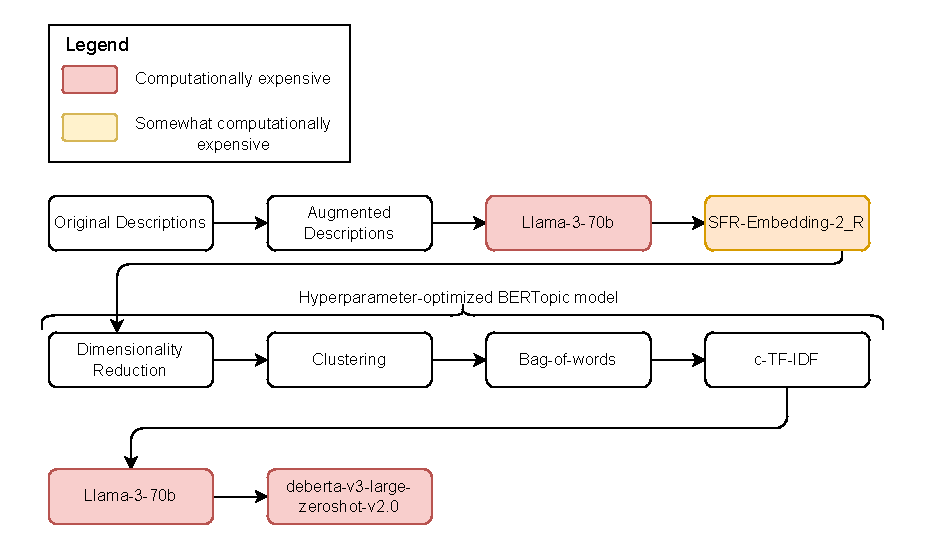
\includegraphics[width=\textwidth]{figures/tag_generation_pipeline_specifics.pdf}
    \caption{Tag generation pipeline specifics}
    \label{fig:tag_generation_pipeline_specifics}
\end{figure}

\subsection{Results}
We now show the results of the output of the tag generation pipeline. \cref{fig:top_50_frequency} shows the top 50 regular tags by frequency, while \cref{fig:top_50_overarching_frequency} shows the top 50 overarching tags by frequency. We see that the tags are quite diverse, covering a wide range of topics. The regular tags are more specific, while the overarching tags are more general.

\begin{figure}[h]
    \centering
    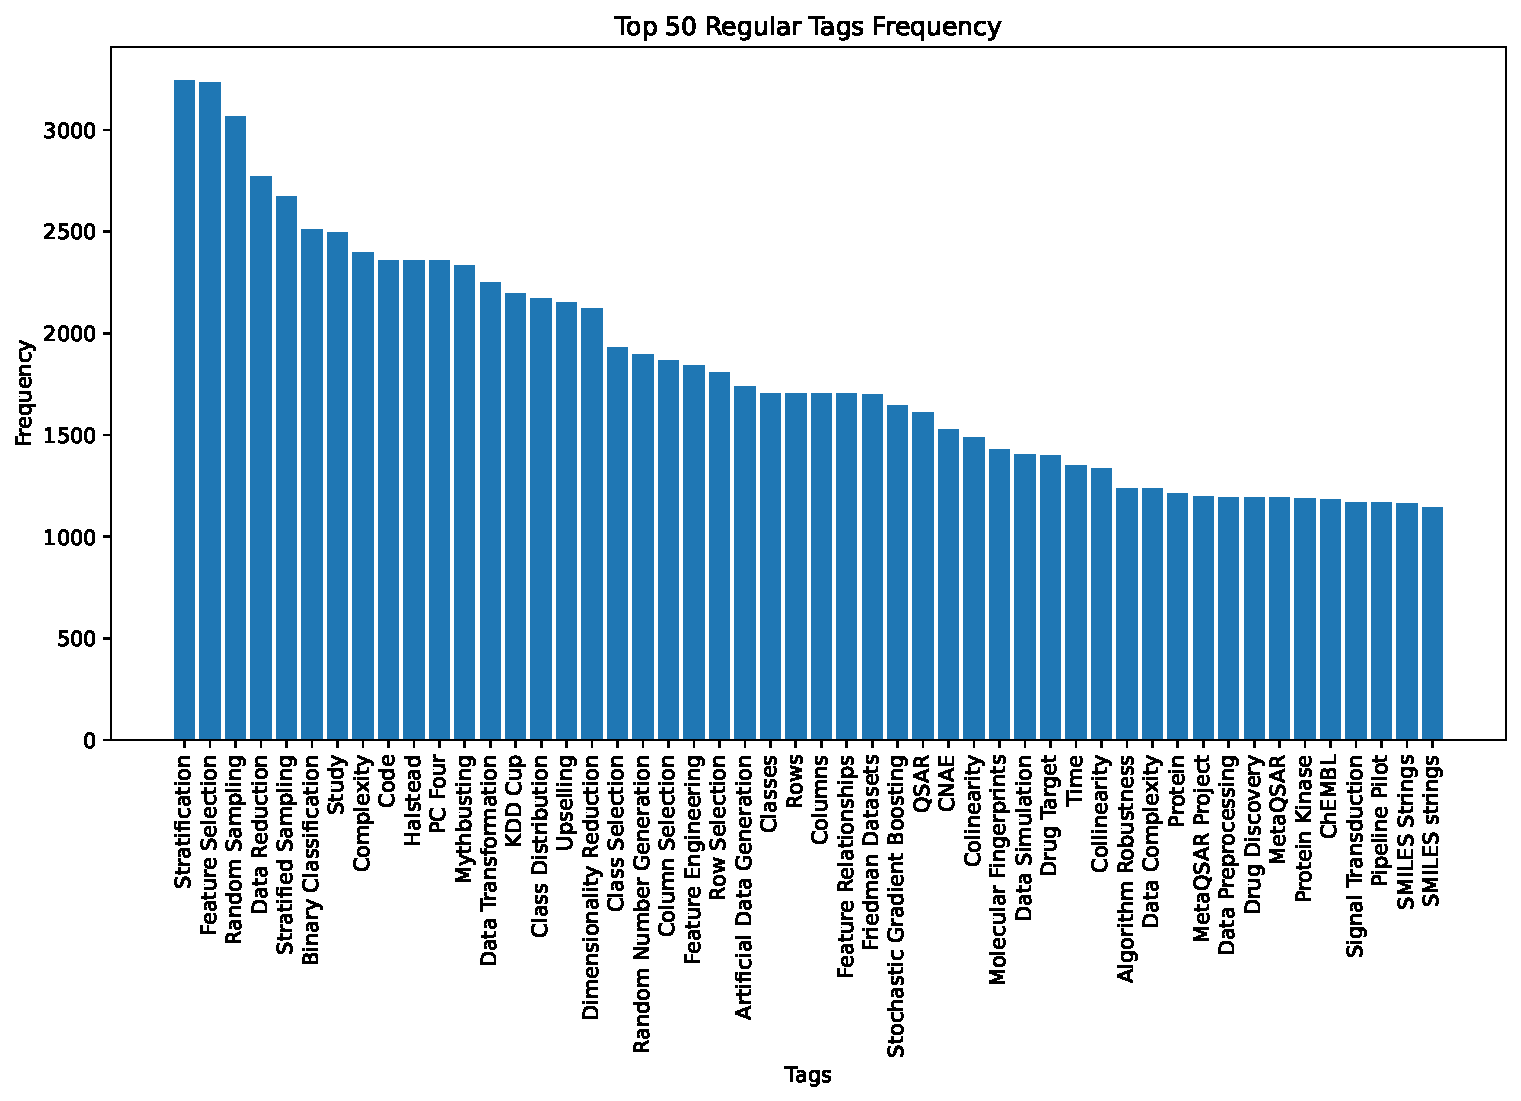
\includegraphics[width=\textwidth]{figures/top_50_frequency.pdf}
    \caption{Top 50 tags by frequency}
    \label{fig:top_50_frequency}
\end{figure}

\begin{figure}[h]
    \centering
    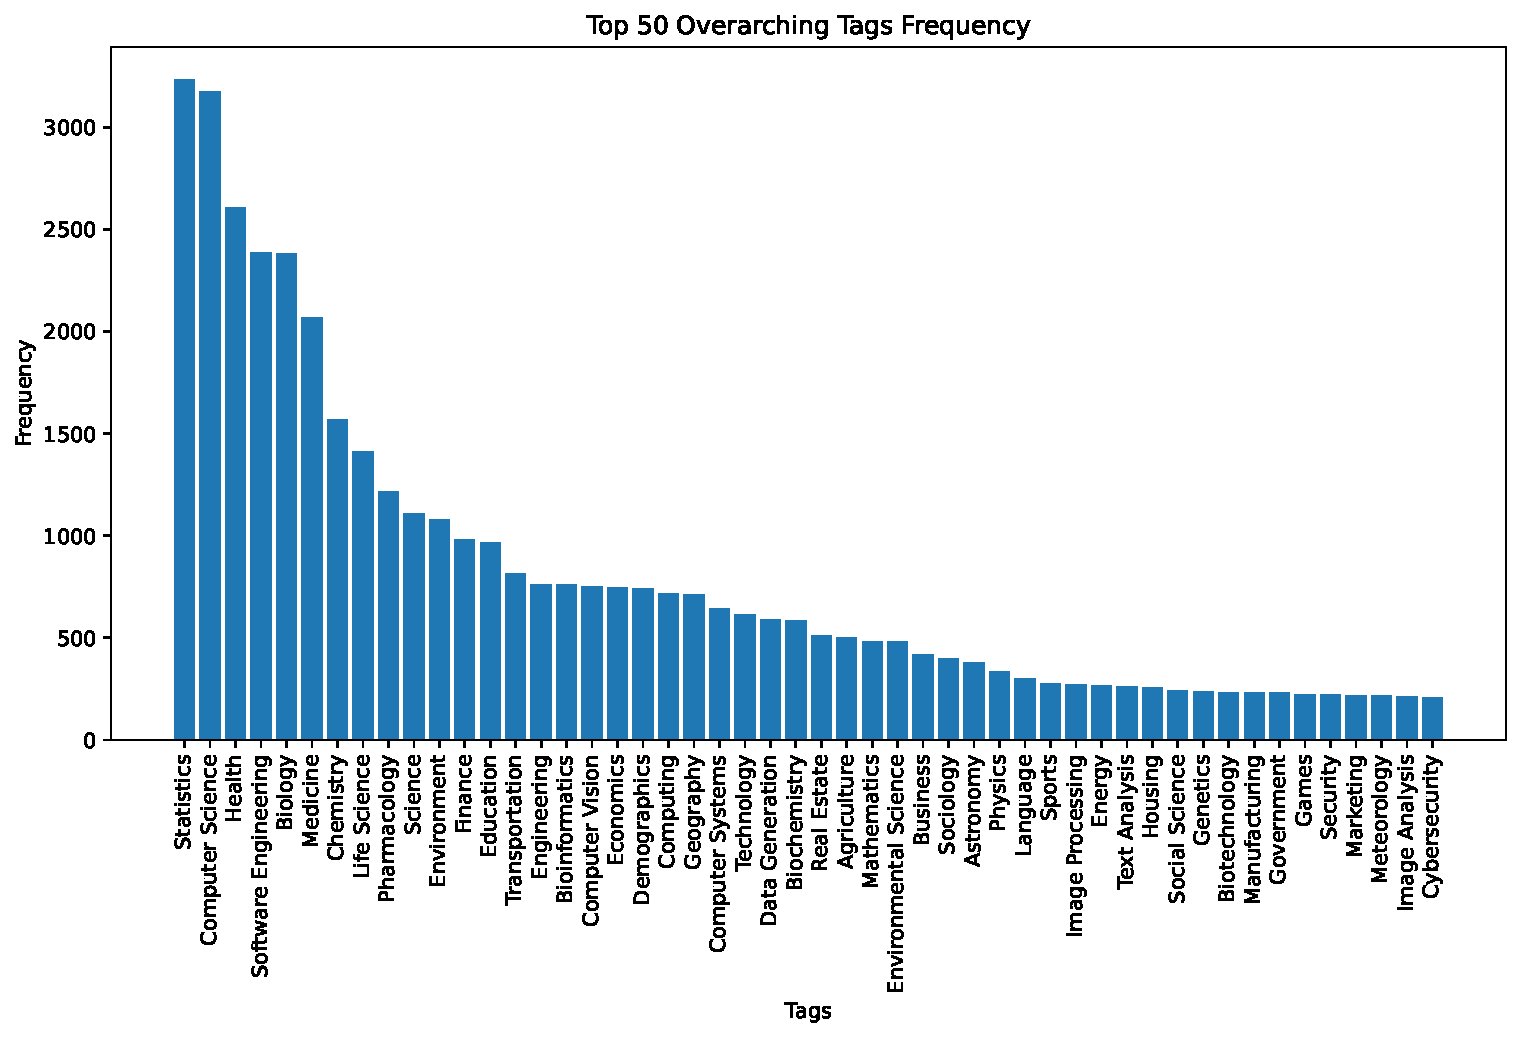
\includegraphics[width=\textwidth]{figures/top_50_overarching_frequency.pdf}
    \caption{Top 50 overarching tags by frequency}
    \label{fig:top_50_overarching_frequency}
\end{figure}

Investigating the tag counts in more detail, we see that the distribution of the tags is highly skewed. \cref{fig:box_plot_tag_counts} shows a box plot of the tag counts, while \cref{fig:box_plot_overarching_tag_counts} shows a box plot of the overarching tag counts. We see that the majority of tags have a low count, with a few tags having a very high count. This is expected, as natural language has been found to follow Zipf's law (Zipfian distribution), where a few terms are very common, while the majority of terms are rare \cite{zipf_psycho-biology_1935, piantadosi_zipfs_2014}.

\begin{figure}[h]
    \centering
    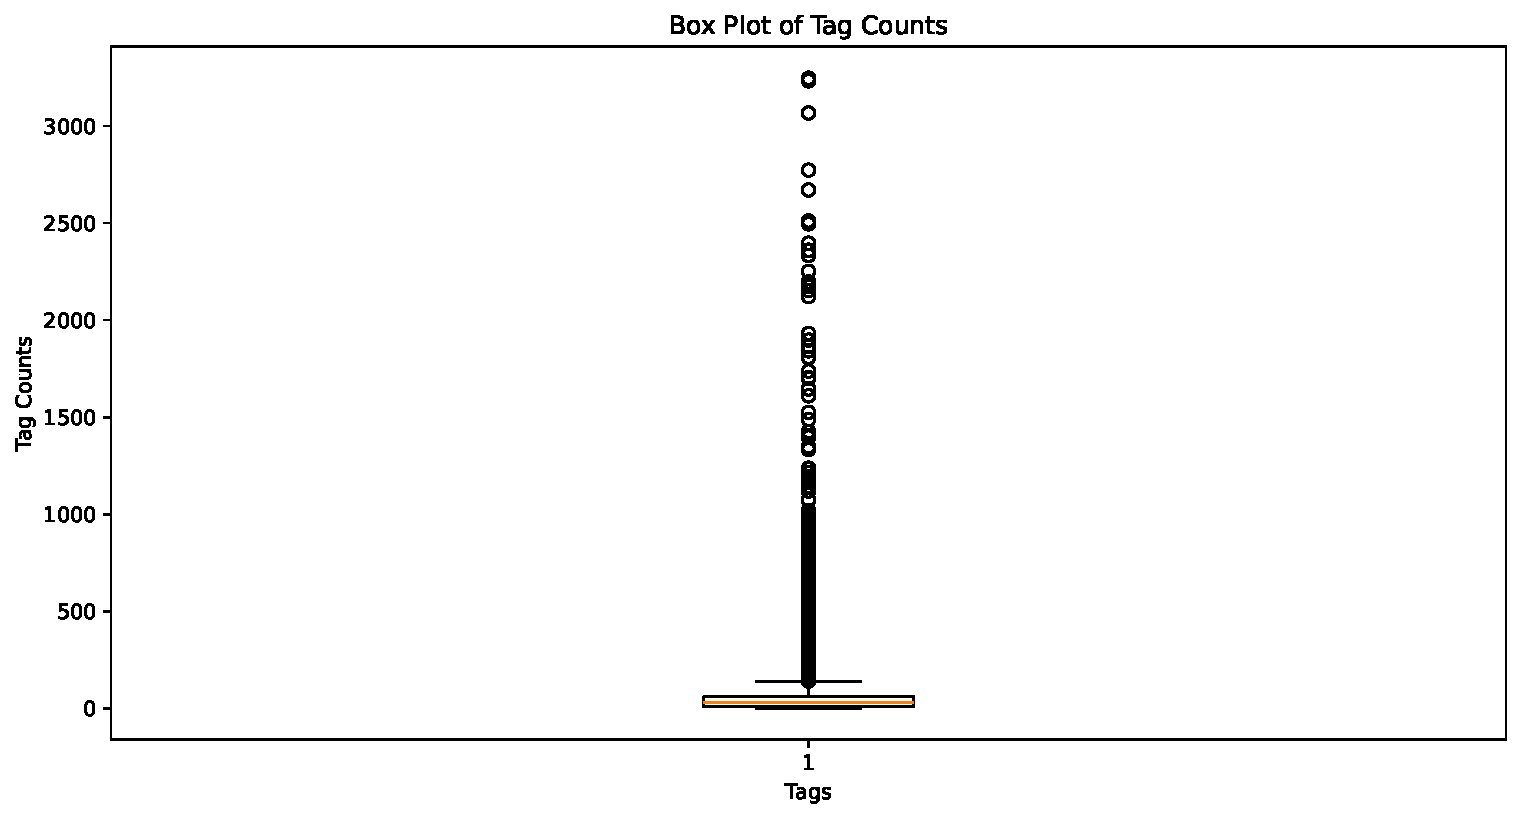
\includegraphics[width=\textwidth]{figures/box_plot_tag_counts.pdf}
    \caption{Box plot of tag counts}
    \label{fig:box_plot_tag_counts}
\end{figure}

\begin{figure}[h]
    \centering
    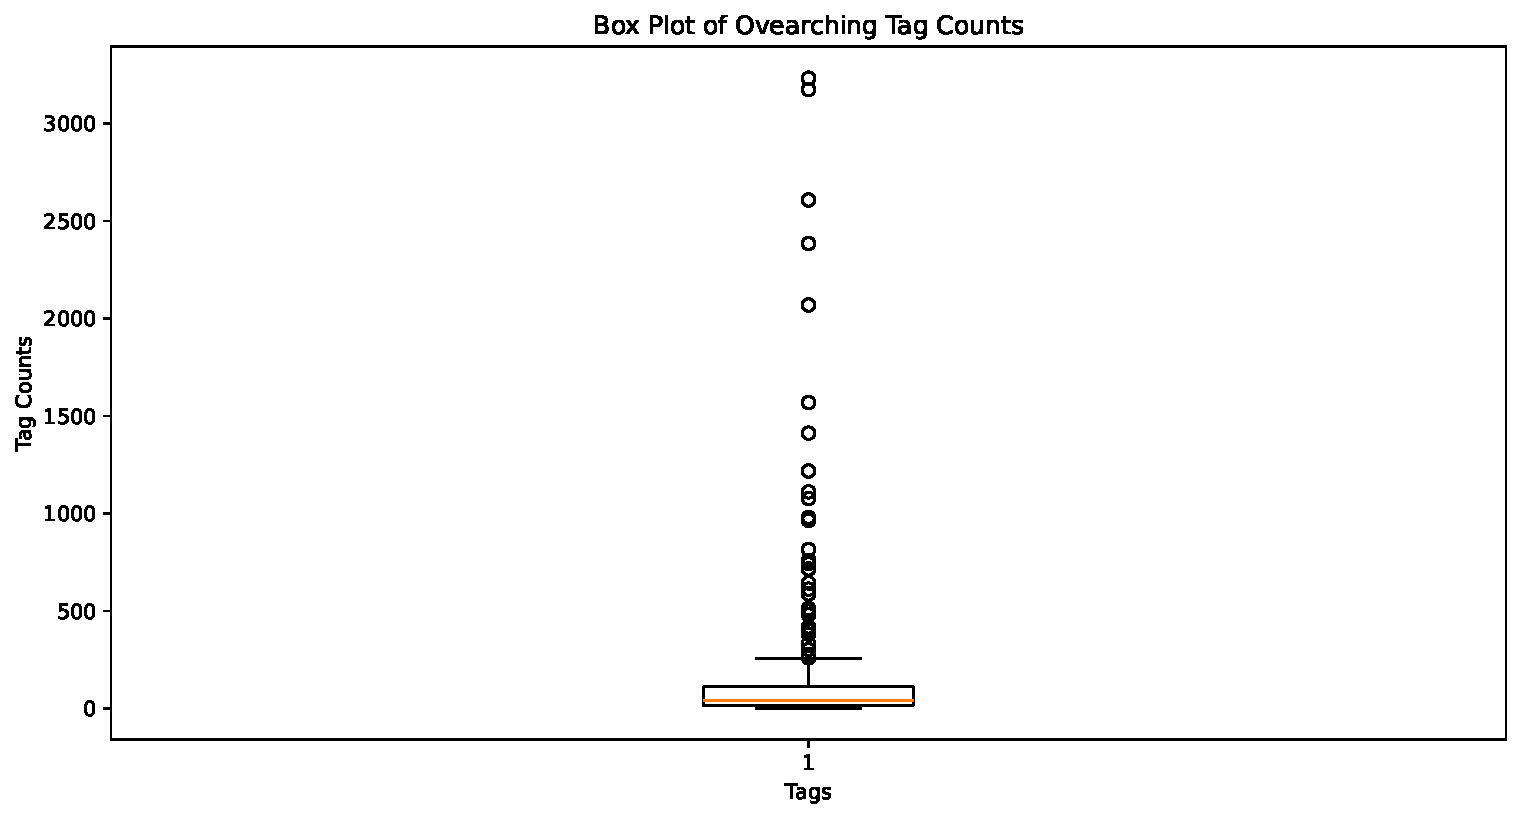
\includegraphics[width=\textwidth]{figures/box_plot_overarching_tag_counts.pdf}
    \caption{Box plot of overarching tag counts}
    \label{fig:box_plot_overarching_tag_counts}
\end{figure}

We observe the same pattern when looking at histograms of the tag counts. \cref{fig:histogram_tag_counts} shows the histogram of tag counts, while \cref{fig:histogram_tag_counts_log} shows the histogram of tag counts on a log scale. We see that the distribution is highly skewed, with a few tags having a very high count. In \cref{fig:histogram_overarching_tag_counts} and \cref{fig:histogram_overarching_tag_counts_log}, we see the same pattern for the overarching tags. It is important to note that the number of regular tags is approximately 6300 and the number of overarching tags is approximately 300. This is also expected, as the overarching tags are more general and should cover a wider range of topics.

\begin{figure}[h]
    \centering
    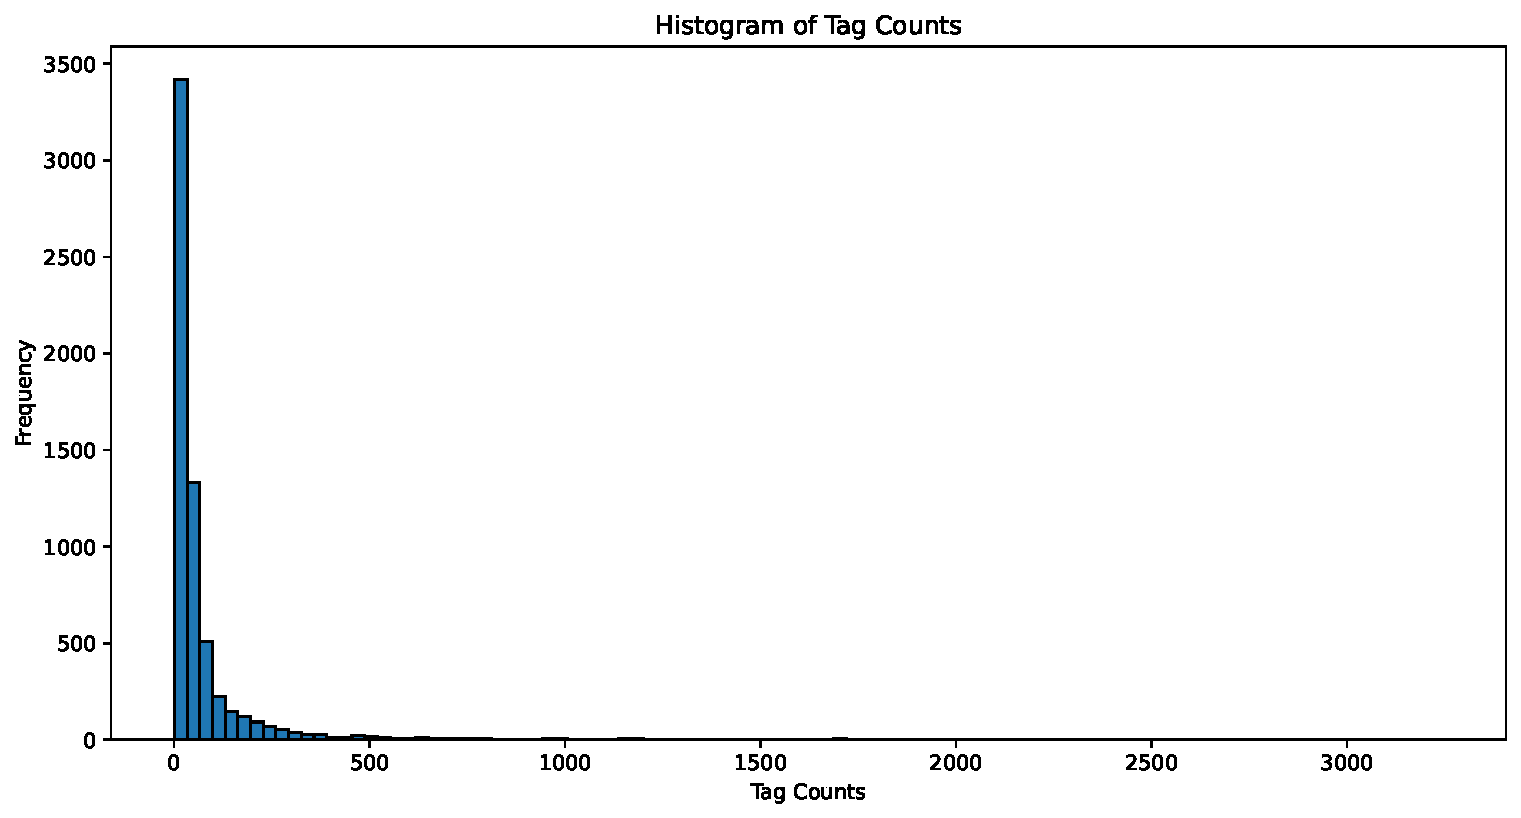
\includegraphics[width=\textwidth]{figures/histogram_tag_counts.pdf}
    \caption{Histogram of tag counts}
    \label{fig:histogram_tag_counts}
\end{figure}

\begin{figure}[h]
    \centering
    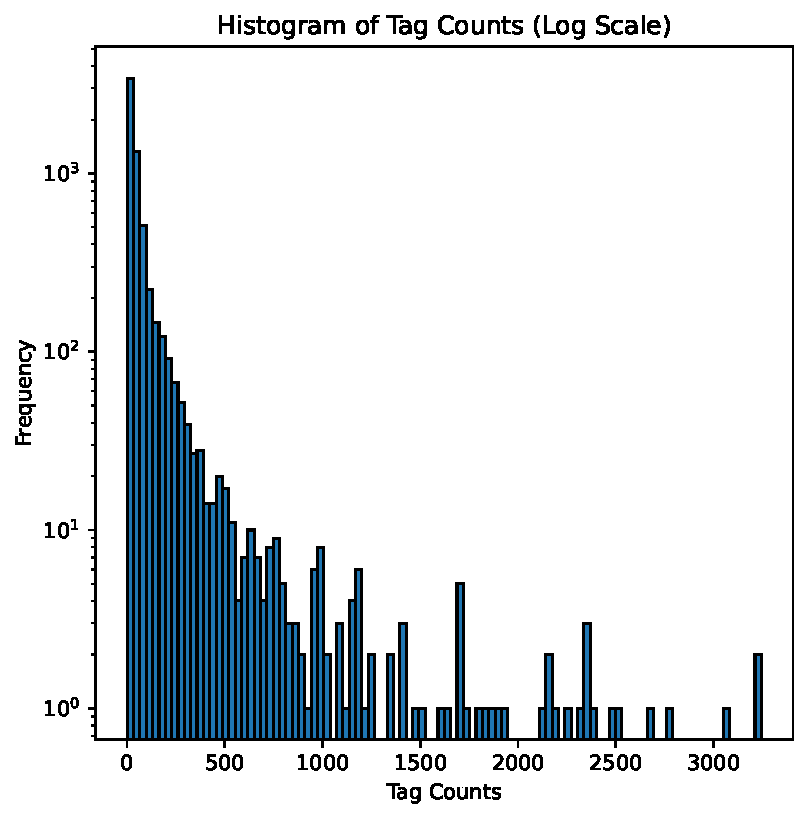
\includegraphics[width=\textwidth]{figures/histogram_tag_counts_log.pdf}
    \caption{Histogram of tag counts (log scale)}
    \label{fig:histogram_tag_counts_log}
\end{figure}

\begin{figure}[h]
    \centering
    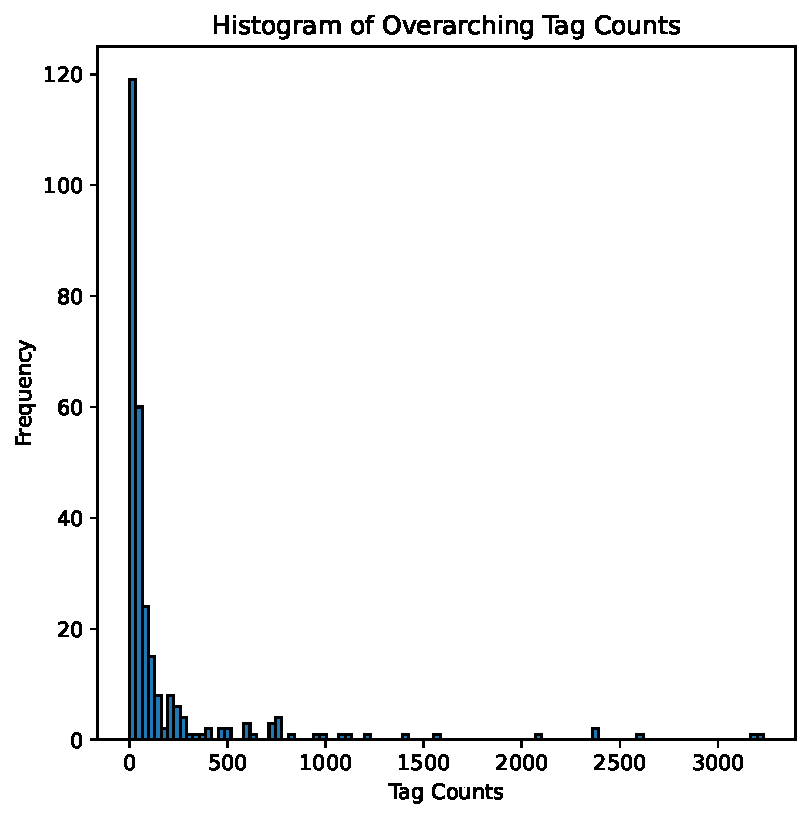
\includegraphics[width=\textwidth]{figures/histogram_overarching_tag_counts.pdf}
    \caption{Histogram of overarching tag counts}
    \label{fig:histogram_overarching_tag_counts}
\end{figure}

\begin{figure}[h]
    \centering
    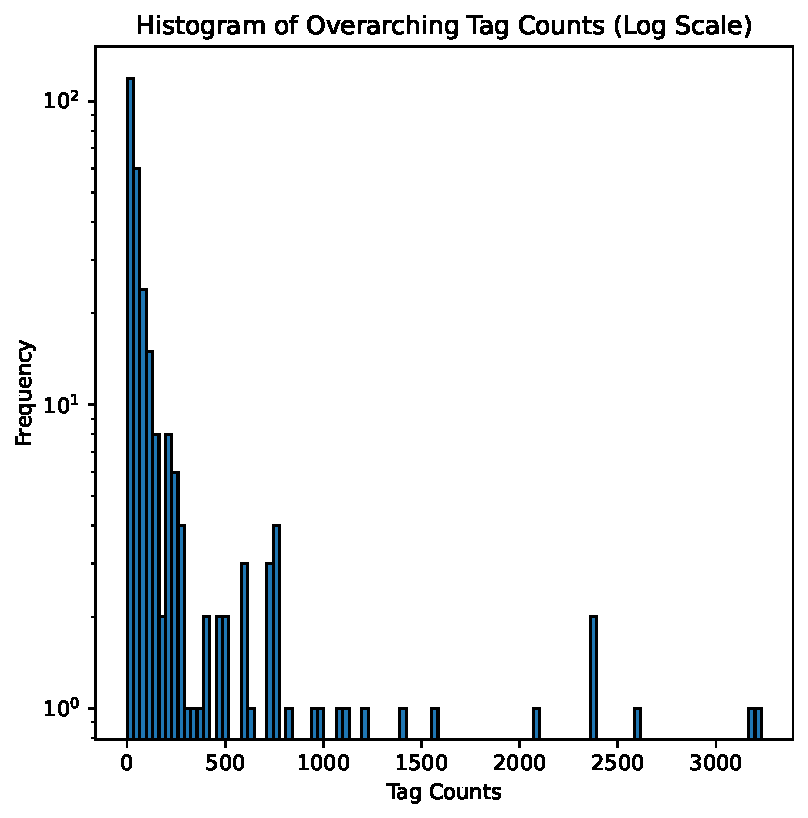
\includegraphics[width=\textwidth]{figures/histogram_overarching_tag_counts_log.pdf}
    \caption{Histogram of overarching tag counts (log scale)}
    \label{fig:histogram_overarching_tag_counts_log}
\end{figure}

We now turn to investigating the tag scores, which are a measure from 0 to 1 that the zeroshot text classifier assigns to each tag based on each individual description. \cref{fig:histogram_scores} shows the histogram of tag scores, while \cref{fig:histogram_overarching_scores} shows the histogram of overarching tag scores. We see that the distribution of scores is skewed, with a few tags having a very low score (close to 0) and a few tags having a very high score (close to 1), with the remaining tags having scores in between. This means that the zeroshot text classifier is filtering out tags that are not relevant to the descriptions, while assigning high scores to tags that are relevant.

\begin{figure}[h]
    \centering
    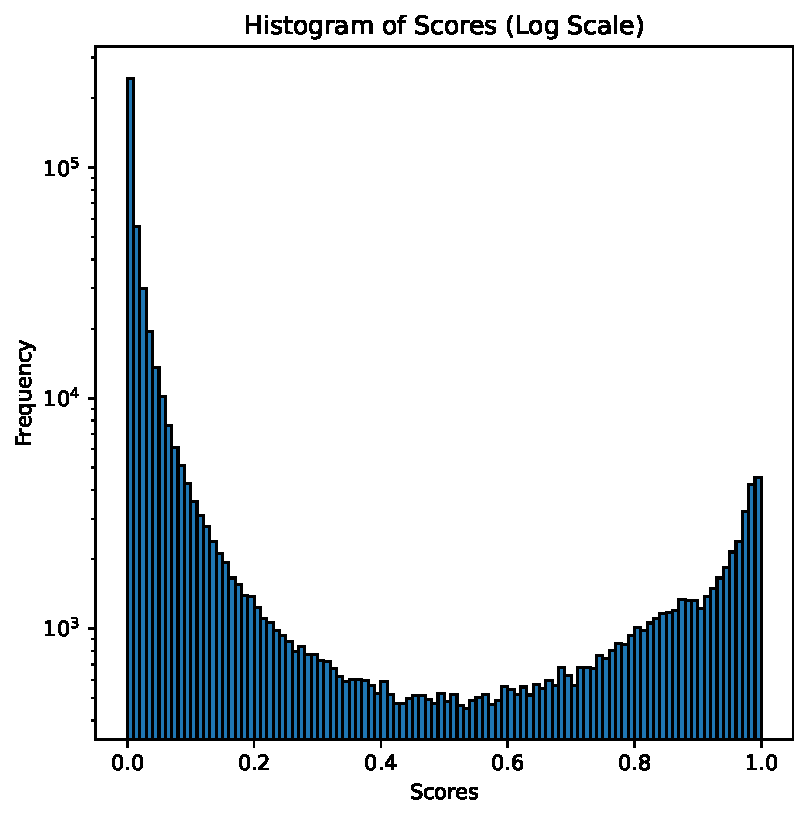
\includegraphics[width=\textwidth]{figures/histogram_scores.pdf}
    \caption{Histogram of tag scores}
    \label{fig:histogram_scores}
\end{figure}

\begin{figure}[h]
    \centering
    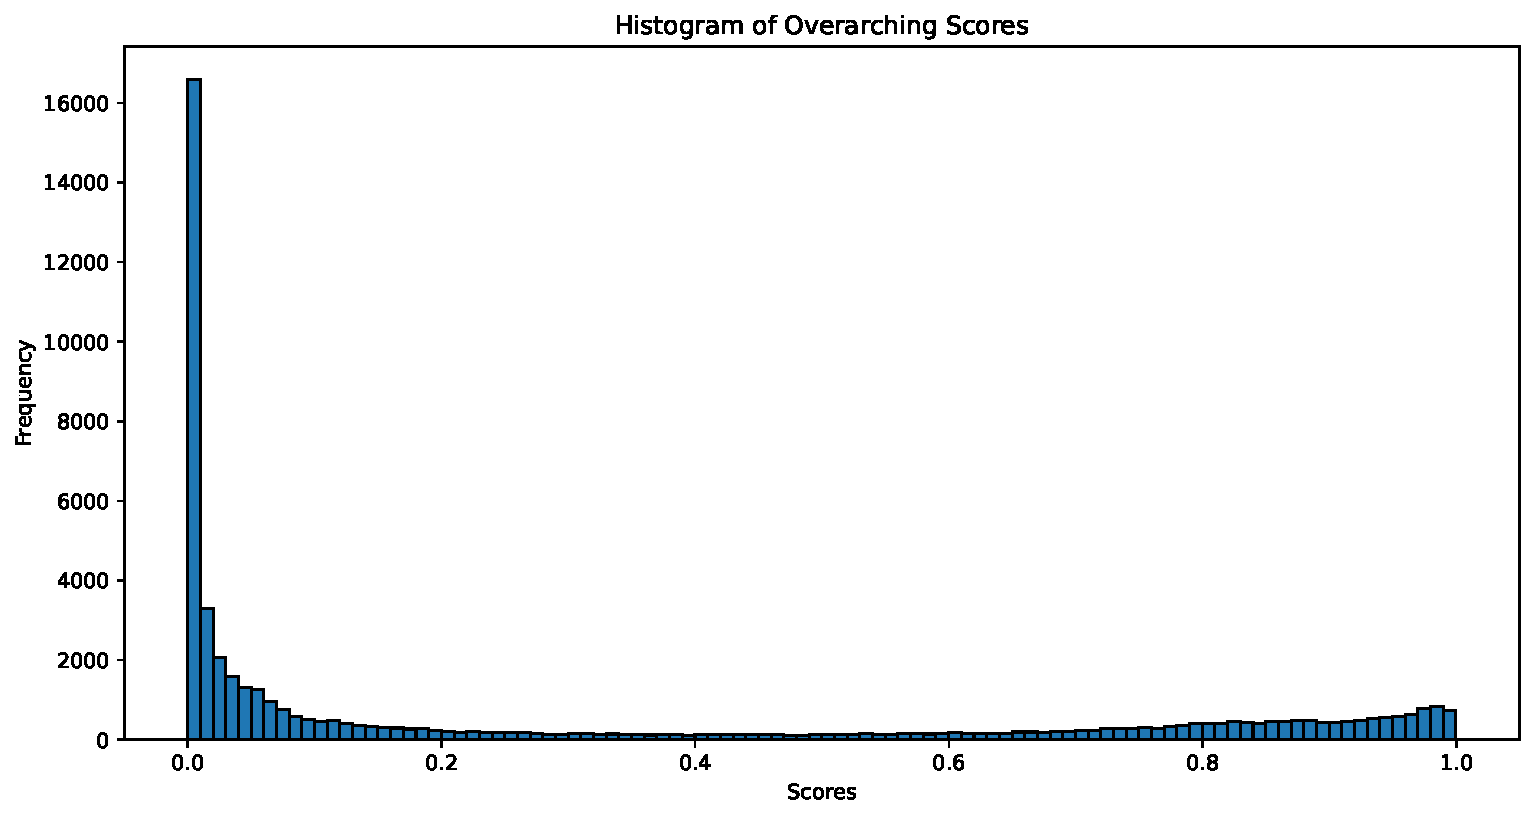
\includegraphics[width=\textwidth]{figures/histogram_overarching_scores.pdf}
    \caption{Histogram of overarching tag scores}
    \label{fig:histogram_overarching_scores}
\end{figure}

\section{Human evaluation}
In this section, we present the results of the human evaluation based on the definition of the study design in \cref{sec:human_evaluation}.

\subsection{Materials}
The same dataset descriptions were used across all three surveys to maintain consistency. Based on a pilot study, we selected three texts for the \textit{Individual Document Evaluation} stage and two for the \textit{Document Pair Evaluation} stage. The selection criteria focused on appropriate length and complexity to ensure participant comprehension. This number of texts allowed participants to complete the survey within approximately 45 minutes, balancing the need for sufficient data collection while preventing participant fatigue.

For brevity, we include only a few examples of the text-tag pairs used in the surveys. All three surveys can be found in the \href{https://github.com/ivangermanov/openml-tags}{GitHub repository} \cite{germanov_topic_modeling_of_2024} under the names of \texttt{proposed\_model\_survey.pdf}, \texttt{baseline\_survey.pdf}, and \texttt{human\_generated\_survey.pdf}.

An example text from the first stage, \textit{Individual Document Evaluation}:

\begin{quote}
    \textbf{FOREX USD/JPY Minute High}

    This dataset contains historical price data of the FOREX USD/JPY from Dukascopy. Each instance, or row, represents one candlestick of one minute. The dataset spans from January first to December thirteenth and does not include weekends, as the FOREX market is not traded on weekends. The timezone of the feature Timestamp is Europe/Amsterdam.
\end{quote}

This text was contained in all three surveys, and for each survey, a different set of tags was provided. \cref{tab:tag_comparison} shows a comparison of tags for different models.

\begin{table}[h]
    \centering
    \begin{tabular}{|>{\raggedright\arraybackslash}p{4cm}|>{\raggedright\arraybackslash}p{4cm}|>{\raggedright\arraybackslash}p{4cm}|}
        \hline
        \textbf{Proposed Model} & \textbf{Human-Generated} & \textbf{Baseline Model} \\ \hline
        Historical Price Data   & Historical Price Data    & Thyrotropin             \\ \hline
        Minute Interval         & Forex                    & Minute                  \\ \hline
        Historical Data         & USD/JPY                  & USD                     \\ \hline
        Forex                   & Currency Pairs           & Releasing               \\ \hline
        Candlestick             & Yearly Data              & High                    \\ \hline
        Minute                  & Finance                  & Bid                     \\ \hline
        High                    & Minute High              & Ask                     \\ \hline
    \end{tabular}
    \caption{Comparison of tags for different models}
    \label{tab:tag_comparison}
\end{table}

For the first task, \textit{Intruder Detection}, an intruder tag, which the participant had to identify, was added to the set of tags for each text. The intruder tag was selected at random from the tags of another OpenML dataset.

In the second task, \textit{Tag Quality Assessment}, for each tag, participants were asked to rate the relevance and generality. For each tag set, participants were asked to rate the coverage.

In the second stage, \textit{Document Pair Evaluation}, participants were provided pairs of texts. For example, one pair consisted of the following two texts:

\begin{quote}
    \textbf{Movies on Netflix, Prime Video, Hulu, and Disney+}

    This dataset is an amalgamation of data that was scraped, comprising a comprehensive list of movies available on various streaming platforms, and the IMDb dataset, which provides inspiration for analysis.

    Which streaming platform or platforms can I find this movie on? This dataset allows us to explore the availability of movies across different streaming services. Additionally, we can examine the average IMDb rating of movies produced in a specific country, providing insights into the quality of films from different regions.

    \textbf{Popular Movies of IMDb}

    TMDB.org is a crowd-sourced movie information database widely used by various film-related consoles, sites, and apps, such as XBMC, MythTV, and Plex. Dozens of media managers, mobile apps, and social sites utilize its API. At the time of writing, TMDB lists a substantial number of films, which is considerably fewer than IMDb. While not as comprehensive as IMDb, it holds extensive information for most popular and Hollywood films.
\end{quote}

In the first task, \textit{Common Tags Identification}, participants were asked to identify tags that were common to both texts, i.e., the intersection of the two tag sets. For instance, for the two tag sets in \cref{tab:tag_comparison_two_datasets}, the common tags were \textit{Film}, \textit{Entertainment}, \textit{Movies}, and \textit{Media} (as predicted by the model).

\begin{table}[h]
    \centering
    \begin{tabular}{|>{\raggedright\arraybackslash}p{6cm}|>{\raggedright\arraybackslash}p{6cm}|}
        \hline
        \textbf{Movies on Netflix, Prime Video, Hulu, and Disney+} & \textbf{Popular Movies of IMDb} \\ \hline
        Film                                                       & Entertainment                   \\ \hline
        Media                                                      & Technology                      \\ \hline
        Entertainment                                              & Film                            \\ \hline
        Movies                                                     & Media                           \\ \hline
        Film Industry                                              & Movies                          \\ \hline
        Streaming Platforms                                        & Popular Movies                  \\ \hline
                                                                   & Film Information                \\ \hline
    \end{tabular}
    \caption{Comparison of tags for two datasets}
    \label{tab:tag_comparison_two_datasets}
\end{table}


In the second task, \textit{Shared Coverage Assessment}, participants were asked to rate the shared coverage of the tags for both texts.

\subsection{Participants}
For the \textit{proposed model} survey, we recruited 21 participants, all of whom completed the survey. For the \textit{baseline model} survey, we recruited 19 participants, and for the \textit{human-generated} survey, we recruited 18 participants. There was a large overlap between the participants in the three surveys, with 93.3\% of participants completing all three surveys.

As for the background of the participants, \cref{fig:education_pie} shows the education level of the participants. We see that the majority of participants have a Bachelor's degree, followed by a Master's degree. This is expected, as the aim of the study was to recruit individuals with a background that aligns with the background of OpenML users.


\begin{figure}[h]
    \centering
    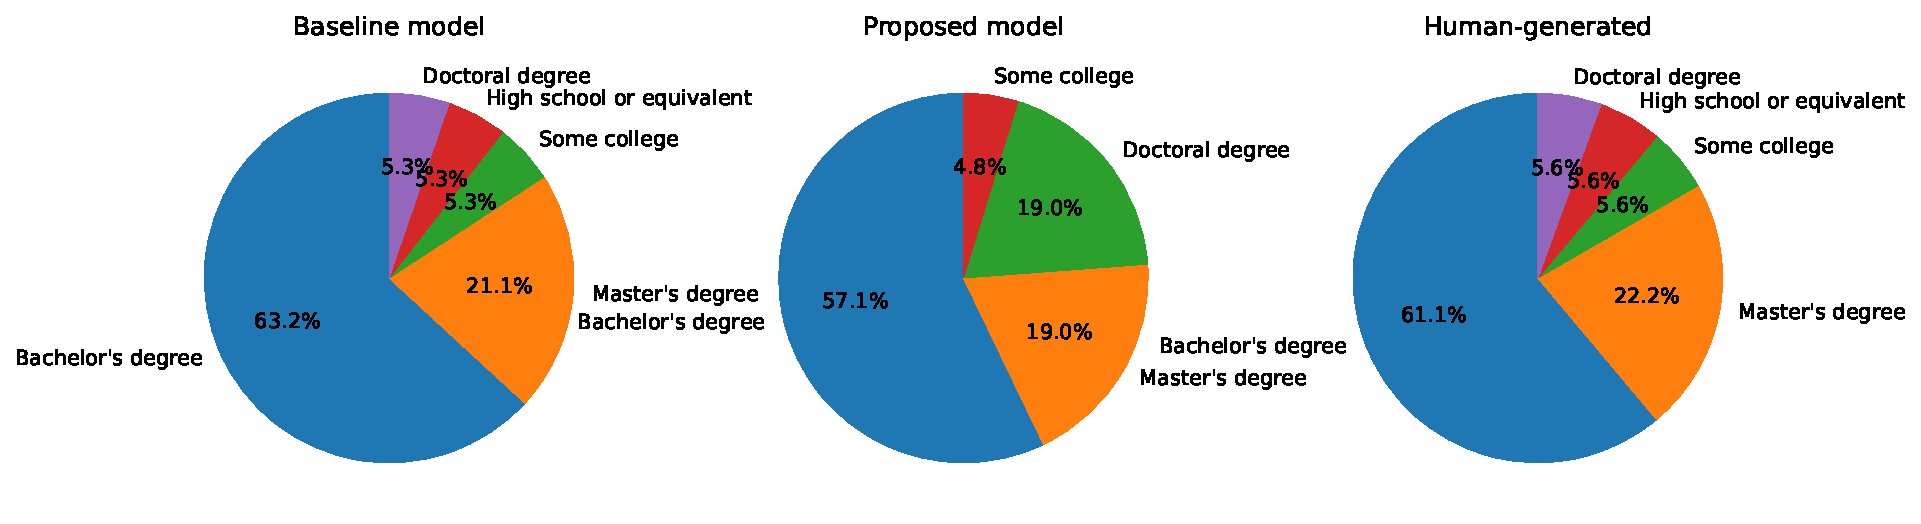
\includegraphics[width=\textwidth]{figures/education_pie.pdf}
    \caption{Education level of participants}
    \label{fig:education_pie}
\end{figure}

\cref{fig:age_range_pie} shows the age range of the participants. We see that the majority of participants are between 25 and 34 years old.

\begin{figure}[h]
    \centering
    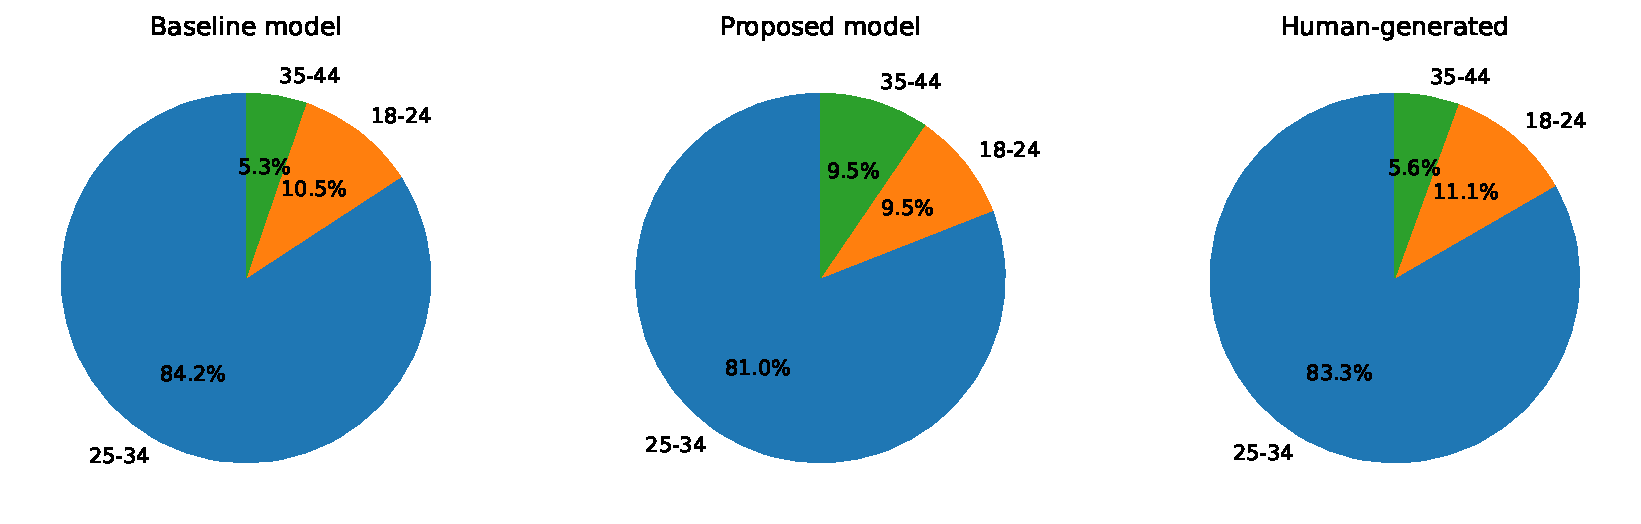
\includegraphics[width=\textwidth]{figures/age_range_pie.pdf}
    \caption{Age range of participants}
    \label{fig:age_range_pie}
\end{figure}

\cref{fig:english_prof_pie} shows the English proficiency of the participants. We see that the majority of participants possess a high level of English proficiency.

\begin{figure}[h]
    \centering
    \includegraphics[width=\textwidth]{figures/english_prof_pie.pdf}
    \caption{English proficiency of participants}
    \label{fig:english_prof_pie}
\end{figure}

\subsection{Results}
\subsubsection{Stage 1 — Task 1: Intruder Detection}
\cref{fig:intruder_detection_results} presents the intruder detection results for all three texts (\textit{League of Legends}, \textit{Forex} and \textit{Lung Cancer}), for all three surveys. The proposed model performed notably better than the baseline model, but slightly lagged behind the human-generated tags. The human-generated tags achieved the highest performance with a perfect score. These results indicate that human-generated tags were of higher quality, as participants more readily identified the intruder tags. This higher detection suggests that intruder tags were less related to the source text, demonstrating greater cohesion among the human-generated tag sets.

\begin{figure}[h]
    \centering
    \includegraphics[width=\textwidth]{figures/intruder_detection_results.pdf}
    \caption{Intruder detection results}
    \label{fig:intruder_detection_results}
\end{figure}

\subsubsection{Stage 1 — Task 2: Tag Quality Assessment}
\cref{fig:tags_analysis_comparison_relevance,fig:tags_analysis_comparison_generality,fig:tags_analysis_comparison_coverage} show the tag quality assessment results for the baseline model, the proposed model, and the human-generated tags, respectively. The histograms display the distribution of scores for relevance, generality, and coverage across all surveys, combining data from all three texts. For each measure, we include the mean scores, standard deviations, and 95\% confidence intervals.

\begin{figure}[h]
    \centering
    \includegraphics[width=0.89\textwidth]{figures/tags_analysis_relevance_comparison.pdf}
    \caption{Aggregated relevance scores by model}
    \label{fig:tags_analysis_comparison_relevance}
\end{figure}

\begin{figure}[h]
    \centering
    \includegraphics[width=0.89\textwidth]{figures/tags_analysis_generality_comparison.pdf}
    \caption{Aggregated generality scores by model}
    \label{fig:tags_analysis_comparison_generality}
\end{figure}

\begin{figure}[h]
    \centering
    \includegraphics[width=0.89\textwidth]{figures/tags_analysis_coverage_comparison.pdf}
    \caption{Aggregated coverage scores by model}
    \label{fig:tags_analysis_comparison_coverage}
\end{figure}

% \begin{figure}[h]
%     \centering
%     \subfloat[Relevance scores]{\includegraphics[width=0.5\textwidth]{figures/tags_analysis_baseline_relevance.pdf}\label{fig:tags_analysis_baseline_relevance}}
%     \hfill
%     \subfloat[Generality scores]{\includegraphics[width=0.5\textwidth]{figures/tags_analysis_baseline_generality.pdf}\label{fig:tags_analysis_baseline_generality}}

%     \subfloat[Coverage scores]{\includegraphics[width=0.5\textwidth]{figures/tags_analysis_baseline_coverage.pdf}\label{fig:tags_analysis_baseline_coverage}}
%     \caption{Tag quality assessment results for the baseline model}
%     \label{fig:tags_analysis_baseline}
% \end{figure}

% \begin{figure}[h]
%     \centering
%     \subfloat[Relevance scores]{\includegraphics[width=0.5\textwidth]{figures/tags_analysis_model_relevance.pdf}\label{fig:tags_analysis_model_relevance}}
%     \hfill
%     \subfloat[Generality scores]{\includegraphics[width=0.5\textwidth]{figures/tags_analysis_model_generality.pdf}\label{fig:tags_analysis_model_generality}}

%     \subfloat[Coverage scores]{\includegraphics[width=0.5\textwidth]{figures/tags_analysis_model_coverage.pdf}\label{fig:tags_analysis_model_coverage}}
%     \caption{Tag quality assessment results for the proposed model}
%     \label{fig:tags_analysis_proposed}
% \end{figure}

% \begin{figure}[h]
%     \centering
%     \subfloat[Relevance scores]{\includegraphics[width=0.5\textwidth]{figures/tags_analysis_human_relevance.pdf}\label{fig:tags_analysis_human_relevance}}
%     \hfill
%     \subfloat[Generality scores]{\includegraphics[width=0.5\textwidth]{figures/tags_analysis_human_generality.pdf}\label{fig:tags_analysis_human_generality}}

%     \subfloat[Coverage scores]{\includegraphics[width=0.5\textwidth]{figures/tags_analysis_human_coverage.pdf}\label{fig:tags_analysis_human_coverage}}
%     \caption{Tag quality assessment results for the human-generated tags}
%     \label{fig:tags_analysis_human}
% \end{figure}

Analysis of the scoring metrics revealed that the proposed model demonstrated superior performance compared to the baseline model. For relevance scores (higher is better), the baseline model achieved a mean of 2.39, while the proposed model achieved 3.63, which is closer to the human-generated tags' score of 3.95. Regarding generality, where larger standard deviations indicate a better balance between general and specific tags, the proposed model (SD = 1.40) performed better than the baseline (SD = 1.33) and nearly matched human-generated tags (SD = 1.41). In terms of coverage, the proposed model (mean = 4.46) outperformed the baseline model (mean = 2.65) and was close to the human-generated tags (mean = 4.54).

The human-generated tags achieved the best scores in relevance, generality and coverage, indicating that the human-generated tags were of higher quality. The proposed model outperformed the baseline model by a wide margin, and only somewhat lagged behind the human-generated tags. This suggests that the proposed model was able to generate better tags than the baseline model, but still not quite as high-quality as human-generated tags.

Another notable observation (\cref{fig:tags_correlations}) is the correlation between relevance and generality scores. For the baseline model, the correlation was -0.42, for the proposed model, it was -0.59, and for human-generated tags, it was -0.19. This indicates that evaluators found more specific tags to be more relevant, which is expected, as more specific tags are more likely to be relevant to the text. However, the inclusion of more general tags can also be beneficial, as they provide a broader context.

\begin{figure}[h]
    \centering
    \subfloat[Baseline model]{\includegraphics[width=0.45\textwidth]{figures/tags_correlations_baseline.pdf}\label{fig:tags_correlations_baseline}}
    \hfill
    \subfloat[Proposed model]{\includegraphics[width=0.45\textwidth]{figures/tags_correlations_model.pdf}\label{fig:tags_correlations_model}}

    \subfloat[Human-generated]{\includegraphics[width=0.45\textwidth]{figures/tags_correlations_human.pdf}\label{fig:tags_correlations_human}}
    \caption{Relevance and generality correlations comparison}
    \label{fig:tags_correlations}
\end{figure}

Additionally, we inspect the aggregated relevance and generality scores by tag type (regular vs. overarching tags, as explained in \cref{sec:tag_generation}) in \cref{fig:tags_analysis_human_multiple_documents} for human-generated tags and in \cref{fig:tags_analysis_model_multiple_documents} for the proposed model. We see that the relevance scores are higher for regular tags than for overarching tags, while the generality scores are higher for overarching tags than for regular tags. This second observation indicates that the pipeline we designed was successful in generating more specific tags for regular tags and more general tags for overarching tags.

\begin{figure}[h]
    \centering
    \subfloat[Aggregated relevance scores]{\includegraphics[width=0.5\textwidth]{figures/tags_analysis_human_multiple_documents_relevance.pdf}\label{fig:tags_analysis_human_multiple_documents_relevance}}
    \hfill
    \subfloat[Aggregated generality scores]{\includegraphics[width=0.5\textwidth]{figures/tags_analysis_human_multiple_documents_generality.pdf}\label{fig:tags_analysis_human_multiple_documents_generality}}
    \caption{Aggregated relevance and generality scores by tag type (human-generated)}
    \label{fig:tags_analysis_human_multiple_documents}
\end{figure}

\begin{figure}[h]
    \centering
    \subfloat[Aggregated relevance scores]{\includegraphics[width=0.5\textwidth]{figures/tags_analysis_model_multiple_documents_relevance.pdf}\label{fig:tags_analysis_model_multiple_documents_relevance}}
    \hfill
    \subfloat[Aggregated generality scores]{\includegraphics[width=0.5\textwidth]{figures/tags_analysis_model_multiple_documents_generality.pdf}\label{fig:tags_analysis_model_multiple_documents_generality}}
    \caption{Aggregated relevance and generality scores by tag type (proposed model)}
    \label{fig:tags_analysis_model_multiple_documents}
\end{figure}

The histograms provided here only show the aggregated results across all three texts, across all tags. For readers interested in the details for each individual text or tag, additional information can be found in the \textit{human\_evaluation\_analysis.ipynb} notebook in the \href{https://github.com/ivangermanov/openml-tags}{GitHub repository} \cite{germanov_topic_modeling_of_2024}.

\paragraph{Inter-rater Reliability}
We calculated the inter-rater reliability for the relevance, generality, and coverage scores using multiple metrics, including Fleiss' Kappa, Interclass Correlation Coefficient (ICC) and Krippendorff's Alpha. We do not use Cohen's Kappa, and use Fleiss' Kappa instead, as it is more suitable for multiple raters and multiple categories.

\cref{tab:fleiss_kappa_comparison} shows the Fleiss' Kappa values for the different evaluation metrics for the baseline model, the proposed model, and the human-generated tags. We see that all values are small, indicating slight agreement at best. However, it is important to note that our data are Likert scale data, which are ordinal, and are not handled well by Fleiss' Kappa, as it treats categories as nominal.

\begin{table}[h]
    \centering
    \begin{tabular}{lccc}
        \hline
        \textbf{Evaluation metric} & \textbf{Baseline model} & \textbf{Proposed model} & \textbf{Human-generated} \\
        \hline
        Relevance                  & 0.15              & 0.12                    & 0.04                     \\
        Generality                 & -0.02             & 0.18                    & 0.10                     \\
        Coverage                   & 0.03              & 0.01                    & -0.02                    \\
        Shared Coverage            & 0.03              & 0.06                    & -0.01                    \\
        \hline
    \end{tabular}
    \caption{Fleiss' Kappa values comparison for different evaluation metrics across models}
    \label{tab:fleiss_kappa_comparison}
\end{table}

We also used ICC to assess the consistency of ratings across our raters (\cref{fig:icc_baseline,fig:icc_model,fig:icc_human}). Among the main forms of ICC, ICC(1) assumes random raters and absolute agreement, ICC(2) assumes random raters with consistency agreement, while ICC(3) is designed for fixed raters with consistency agreement. Furthermore, ICC(3,k) specifically measures the reliability of averaged ratings rather than individual ratings. ICC(3,k) is most appropriate for our study design because we have a fixed set of participants rating the same texts across different conditions (baseline, proposed model, and human-generated tags), and we are interested in the reliability of averaged ratings rather than individual ratings. ICC(3,k) accounts for systematic differences in how individual participants use the rating scale while providing reliability estimates for the averaged scores, making it the most suitable choice for comparing the reliability of ratings across our three tag generation methods.

\begin{figure}[h]
    \centering
    \begin{minipage}{.5\textwidth}
        \centering
        \begin{tabular}{lcccl}
            \hline
            \textbf{Type} & \textbf{ICC} & \textbf{F} & \textbf{p} & \textbf{CI95\%} \\
            \hline
            ICC1          & 0.45         & 16.65      & 1.68e-40   & [0.31, 0.64]    \\
            ICC2          & 0.46         & 25.92      & 1.18e-57   & [0.31, 0.65]    \\
            ICC3          & 0.57         & 25.92      & 1.18e-57   & [0.42, 0.74]    \\
            ICC1k         & 0.94         & 16.65      & 1.68e-40   & [0.90, 0.97]    \\
            ICC2k         & 0.94         & 25.92      & 1.18e-57   & [0.89, 0.97]    \\
            ICC3k         & 0.96         & 25.92      & 1.18e-57   & [0.93, 0.98]    \\
            \hline
        \end{tabular}
        \caption*{(a) Relevance}
    \end{minipage}%
    \begin{minipage}{.5\textwidth}
        \centering
        \begin{tabular}{lcccl}
            \hline
            \textbf{Type} & \textbf{ICC} & \textbf{F} & \textbf{p} & \textbf{CI95\%} \\
            \hline
            ICC1          & -0.03        & 0.53       & 0.711      & [-0.04, 0.15]   \\
            ICC2          & 0.00         & 0.99       & 0.416      & [-0.02, 0.17]   \\
            ICC3          & 0.00         & 0.99       & 0.416      & [-0.04, 0.28]   \\
            ICC1k         & -0.87        & 0.53       & 0.711      & [-4.49, 0.78]   \\
            ICC2k         & 0.00         & 0.99       & 0.416      & [-0.56, 0.80]   \\
            ICC3k         & -0.01        & 0.99       & 0.416      & [-1.98, 0.88]   \\
            \hline
        \end{tabular}
        \caption*{(b) Generality}
    \end{minipage}

    \vspace{1em}
    \begin{minipage}{.5\textwidth}
        \centering
        \begin{tabular}{lcccl}
            \hline
            \textbf{Type} & \textbf{ICC} & \textbf{F} & \textbf{p} & \textbf{CI95\%} \\
            \hline
            ICC1          & 0.33         & 10.16      & 1.80e-04   & [0.08, 0.95]    \\
            ICC2          & 0.34         & 21.51      & 7.14e-07   & [0.10, 0.95]    \\
            ICC3          & 0.52         & 21.51      & 7.14e-07   & [0.18, 0.98]    \\
            ICC1k         & 0.90         & 10.16      & 1.80e-04   & [0.61, 1.00]    \\
            ICC2k         & 0.91         & 21.51      & 7.14e-07   & [0.67, 1.00]    \\
            ICC3k         & 0.95         & 21.51      & 7.14e-07   & [0.81, 1.00]    \\
            \hline
        \end{tabular}
        \caption*{(c) Coverage}
    \end{minipage}%
    \begin{minipage}{.5\textwidth}
        \centering
        \begin{tabular}{lcccl}
            \hline
            \textbf{Type} & \textbf{ICC} & \textbf{F} & \textbf{p} & \textbf{CI95\%} \\
            \hline
            ICC1          & 0.04         & 1.69       & 0.202      & [-0.04, 0.99]   \\
            ICC2          & 0.06         & 3.65       & 0.072      & [-0.01, 0.99]   \\
            ICC3          & 0.12         & 3.65       & 0.072      & [-0.02, 0.99]   \\
            ICC1k         & 0.41         & 1.69       & 0.202      & [-2.24, 1.00]   \\
            ICC2k         & 0.55         & 3.65       & 0.072      & [-0.18, 1.00]   \\
            ICC3k         & 0.73         & 3.65       & 0.072      & [-0.64, 1.00]   \\
            \hline
        \end{tabular}
        \caption*{(d) Shared Coverage}
    \end{minipage}
    \caption{ICC values for different rating types (baseline model)}
    \label{fig:icc_baseline}
\end{figure}

\begin{figure}[h]
    \centering
    \begin{minipage}{.5\textwidth}
        \centering
        \begin{tabular}{lcccl}
            \hline
            \textbf{Type} & \textbf{ICC} & \textbf{F} & \textbf{p} & \textbf{CI95\%} \\
            \hline
            ICC1          & 0.34         & 11.93      & 2.88e-30   & [0.22, 0.53]    \\
            ICC2          & 0.35         & 19.27      & 7.72e-47   & [0.22, 0.54]    \\
            ICC3          & 0.47         & 19.27      & 7.72e-47   & [0.32, 0.65]    \\
            ICC1k         & 0.92         & 11.93      & 2.88e-30   & [0.85, 0.96]    \\
            ICC2k         & 0.92         & 19.27      & 7.72e-47   & [0.86, 0.96]    \\
            ICC3k         & 0.95         & 19.27      & 7.72e-47   & [0.91, 0.98]    \\
            \hline
        \end{tabular}
        \caption*{(a) Relevance}
    \end{minipage}%
    \begin{minipage}{.5\textwidth}
        \centering
        \begin{tabular}{lcccl}
            \hline
            \textbf{Type} & \textbf{ICC} & \textbf{F} & \textbf{p} & \textbf{CI95\%} \\
            \hline
            ICC1          & 0.46         & 18.68      & 1.94e-35   & [0.30, 0.68]    \\
            ICC2          & 0.46         & 31.71      & 4.86e-53   & [0.30, 0.69]    \\
            ICC3          & 0.59         & 31.71      & 4.86e-53   & [0.43, 0.78]    \\
            ICC1k         & 0.95         & 18.68      & 1.94e-35   & [0.90, 0.98]    \\
            ICC2k         & 0.95         & 31.71      & 4.86e-53   & [0.90, 0.98]    \\
            ICC3k         & 0.97         & 31.71      & 4.86e-53   & [0.94, 0.99]    \\
            \hline
        \end{tabular}
        \caption*{(b) Generality}
    \end{minipage}

    \vspace{1em}

    \begin{minipage}{.5\textwidth}
        \centering
        \begin{tabular}{lcccl}
            \hline
            \textbf{Type} & \textbf{ICC} & \textbf{F} & \textbf{p} & \textbf{CI95\%} \\
            \hline
            ICC1          & 0.05         & 2.06       & 0.137      & [-0.02, 0.79]   \\
            ICC2          & 0.07         & 5.57       & 0.007      & [0.01, 0.79]    \\
            ICC3          & 0.18         & 5.57       & 0.007      & [0.02, 0.91]    \\
            ICC1k         & 0.51         & 2.06       & 0.137      & [-0.91, 0.99]   \\
            ICC2k         & 0.63         & 5.57       & 0.007      & [0.12, 0.99]    \\
            ICC3k         & 0.82         & 5.57       & 0.007      & [0.27, 1.00]    \\
            \hline
        \end{tabular}
        \caption*{(c) Coverage}
    \end{minipage}%
    \begin{minipage}{.5\textwidth}
        \centering
        \begin{tabular}{lcccl}
            \hline
            \textbf{Type} & \textbf{ICC} & \textbf{F} & \textbf{p} & \textbf{CI95\%} \\
            \hline
            ICC1          & 0.19         & 5.99       & 0.019      & [0.00, 1.00]    \\
            ICC2          & 0.20         & 10.25      & 0.004      & [0.02, 1.00]    \\
            ICC3          & 0.31         & 10.25      & 0.004      & [0.03, 1.00]    \\
            ICC1k         & 0.83         & 5.99       & 0.019      & [0.09, 1.00]    \\
            ICC2k         & 0.84         & 10.25      & 0.004      & [0.34, 1.00]    \\
            ICC3k         & 0.90         & 10.25      & 0.004      & [0.43, 1.00]    \\
            \hline
        \end{tabular}
        \caption*{(d) Shared Coverage}
    \end{minipage}
    \caption{ICC values for different rating types (proposed model)}
    \label{fig:icc_model}
\end{figure}

\begin{figure}[h]
    \centering
    \begin{minipage}{.5\textwidth}
        \centering
        \begin{tabular}{lcccl}
            \hline
            \textbf{Type} & \textbf{ICC} & \textbf{F} & \textbf{p} & \textbf{CI95\%} \\
            \hline
            ICC1          & 0.13         & 3.70       & 5.26e-07   & [0.06, 0.28]    \\
            ICC2          & 0.15         & 8.70       & 7.21e-20   & [0.07, 0.31]    \\
            ICC3          & 0.30         & 8.70       & 7.21e-20   & [0.18, 0.50]    \\
            ICC1k         & 0.73         & 3.70       & 5.26e-07   & [0.52, 0.87]    \\
            ICC2k         & 0.77         & 8.70       & 7.21e-20   & [0.59, 0.89]    \\
            ICC3k         & 0.89         & 8.70       & 7.21e-20   & [0.80, 0.95]    \\
            \hline
        \end{tabular}
        \caption*{(a) Relevance}
    \end{minipage}%
    \begin{minipage}{.5\textwidth}
        \centering
        \begin{tabular}{lcccl}
            \hline
            \textbf{Type} & \textbf{ICC} & \textbf{F} & \textbf{p} & \textbf{CI95\%} \\
            \hline
            ICC1          & 0.34         & 10.38      & 9.38e-21   & [0.20, 0.56]    \\
            ICC2          & 0.35         & 16.76      & 5.01e-32   & [0.21, 0.57]    \\
            ICC3          & 0.47         & 16.76      & 5.01e-32   & [0.31, 0.68]    \\
            ICC1k         & 0.90         & 10.38      & 9.38e-21   & [0.82, 0.96]    \\
            ICC2k         & 0.91         & 16.76      & 5.01e-32   & [0.83, 0.96]    \\
            ICC3k         & 0.94         & 16.76      & 5.01e-32   & [0.89, 0.97]    \\
            \hline
        \end{tabular}
        \caption*{(b) Generality}
    \end{minipage}

    \vspace{1em}
    \begin{minipage}{.5\textwidth}
        \centering
        \begin{tabular}{lcccl}
            \hline
            \textbf{Type} & \textbf{ICC} & \textbf{F} & \textbf{p} & \textbf{CI95\%} \\
            \hline
            ICC1          & -0.02        & 0.59       & 0.560      & [-0.05, 0.55]   \\
            ICC2          & 0.00         & 1.09       & 0.348      & [-0.02, 0.56]   \\
            ICC3          & 0.00         & 1.09       & 0.348      & [-0.04, 0.70]   \\
            ICC1k         & -0.71        & 0.59       & 0.560      & [-5.77, 0.96]   \\
            ICC2k         & 0.05         & 1.09       & 0.348      & [-0.65, 0.96]   \\
            ICC3k         & 0.08         & 1.09       & 0.348      & [-2.78, 0.98]   \\
            \hline
        \end{tabular}
        \caption*{(c) Coverage}
    \end{minipage}%
    \begin{minipage}{.5\textwidth}
        \centering
        \begin{tabular}{lcccl}
            \hline
            \textbf{Type} & \textbf{ICC} & \textbf{F} & \textbf{p} & \textbf{CI95\%} \\
            \hline
            ICC1          & 0.10         & 3.09       & 0.088      & [-0.02, 0.99]   \\
            ICC2          & 0.12         & 4.25       & 0.055      & [-0.01, 0.99]   \\
            ICC3          & 0.15         & 4.25       & 0.055      & [-0.02, 1.00]   \\
            ICC1k         & 0.68         & 3.09       & 0.088      & [-0.78, 1.00]   \\
            ICC2k         & 0.70         & 4.25       & 0.055      & [-0.20, 1.00]   \\
            ICC3k         & 0.76         & 4.25       & 0.055      & [-0.42, 1.00]   \\
            \hline
        \end{tabular}
        \caption*{(d) Shared Coverage}
    \end{minipage}
    \caption{ICC values for different rating types (human-generated)}
    \label{fig:icc_human}
\end{figure}

Looking at the ICC(3,k) values for relevance, where the F-statistic indicates the ratio of between-group to within-group variance (higher values showing stronger rater agreement), we see that the proposed model achieved an ICC of 0.95 ($F=19.27$, $p=7.72\times10^{-47}$, CI$_{95\%}$[0.91,0.98]), the baseline model an ICC of 0.96 ($F=25.92$, $p=1.18\times10^{-57}$, CI$_{95\%}$[0.93,0.98]), and the human-generated tags an ICC of 0.89 ($F=8.70$, $p=7.21\times10^{-20}$, CI$_{95\%}$[0.80,0.95]). For generality, the proposed model performed best with an ICC of 0.97 ($F=31.71$, $p=4.86\times10^{-53}$, CI$_{95\%}$[0.94,0.99]), followed by human-generated tags at 0.94 ($F=16.76$, $p=5.01\times10^{-32}$, CI$_{95\%}$[0.89,0.97]), while the baseline model showed poor reliability with -0.01 ($F=0.99$, $p=0.416$, CI$_{95\%}$[-1.98,0.88]) and a non-significant $p$-value indicating unreliable results. For coverage, the baseline model achieved the highest reliability at 0.95 ($F=21.51$, $p=7.14\times10^{-7}$, CI$_{95\%}$[0.81,1.00]), followed by the proposed model at 0.82 ($F=5.57$, $p=0.007$, CI$_{95\%}$[0.27,1.00]), while human-generated tags performed poorly at 0.08 ($F=1.09$, $p=0.348$, CI$_{95\%}$[-2.78,0.98]) with non-significant results. For shared coverage, the proposed model showed the strongest reliability at 0.90 ($F=10.25$, $p=0.004$, CI$_{95\%}$[0.43,1.00]), followed by human-generated tags at 0.76 ($F=4.25$, $p=0.055$, CI$_{95\%}$[-0.42,1.00]) and the baseline model at 0.73 ($F=3.65$, $p=0.072$, CI$_{95\%}$[-0.64,1.00]), though the latter two had borderline significant $p$-values suggesting less reliable results.

Similar to Fleiss' Kappa, ICC may not be ideal for ordinal data, as it assumes continuous data. This is why Krippendorff's Alpha, which can handle both ordinal and nominal data, is a better choice. \cref{tab:kalpha} shows the Krippendorff's Alpha values for the different evaluation metrics for the baseline model, the proposed model, and the human-generated tags. We see that the baseline model performs best in shared coverage ($\alpha=0.4818$), while showing moderate reliability for generality ($\alpha=0.2863$) and coverage ($\alpha=0.2600$), but lower reliability for relevance ($\alpha=0.1687$). The proposed model shows strongest reliability in coverage ($\alpha=0.5647$), moderate reliability in shared coverage ($\alpha=0.2497$) and relevance ($\alpha=0.2263$), but lower reliability in generality ($\alpha=0.1671$). The human-generated tags show the highest reliability for relevance ($\alpha=0.4692$) and coverage ($\alpha=0.4503$), but lower reliability for generality ($\alpha=0.2044$) and shared coverage ($\alpha=0.1898$). Overall, these values indicate moderate to fair agreement across all three approaches, with different strengths in different evaluation metrics.

\begin{table}[htbp]
    \centering
    \begin{tabular}{lccc}
        \hline
        \textbf{Metric} & \textbf{Baseline model} & \textbf{Proposed model} & \textbf{Human-generated} \\
        \hline
        Relevance       & 0.1687            & 0.2263                  & 0.4692                   \\
        Generality      & 0.2863            & 0.1671                  & 0.2044                   \\
        Coverage        & 0.2600            & 0.5647                  & 0.4503                   \\
        Shared Coverage & 0.4818            & 0.2497                  & 0.1898                   \\
        \hline
    \end{tabular}
    \caption{Krippendorff's Alpha values for different rating types across models}
    \label{tab:kalpha}
\end{table}

\subsubsection{Stage 2 — Task 1: Common Tags Identification}
The confusion matrices in \cref{fig:first_pair_common_tags_confusion_matrix} show the common tags confusion matrix comparison for the first pair of texts. The confusion matrices in \cref{fig:second_pair_common_tags_confusion_matrix} show the common tags confusion matrix comparison for the second pair of texts.

The top-left quadrant of the confusion matrix represents the true positives, i.e., the number of tags that the model predicted as common tags that human evaluators also identified as common tags. The bottom-right quadrant represents the true negatives, i.e., the number of tags that the model predicted as not common tags that human evaluators also identified as not common tags. The top-right quadrant represents the false negatives, i.e., the number of tags that the model predicted as common tags that human evaluators identified as not common tags. The bottom-left quadrant represents the false positives, i.e., the number of tags that the model predicted as not common tags that human evaluators identified as common tags.

\begin{figure}[h]
    \centering
    \subfloat[Baseline model]{\includegraphics[width=0.5\textwidth]{figures/first_pair_common_tags_confusion_matrix_baseline.pdf}\label{fig:first_pair_common_tags_confusion_matrix_baseline}}
    \hfill
    \subfloat[Proposed model]{\includegraphics[width=0.5\textwidth]{figures/first_pair_common_tags_confusion_matrix_model.pdf}\label{fig:first_pair_common_tags_confusion_matrix_model}}

    \subfloat[Human-generated]{\includegraphics[width=0.5\textwidth]{figures/first_pair_common_tags_confusion_matrix_human.pdf}\label{fig:first_pair_common_tags_confusion_matrix_human}}
    \caption{Common tags confusion matrix comparison for the first pair}
    \label{fig:first_pair_common_tags_confusion_matrix}
\end{figure}

\begin{figure}[h]
    \centering
    \subfloat[Baseline model]{\includegraphics[width=0.46\textwidth]{figures/second_pair_common_tags_confusion_matrix_baseline.pdf}\label{fig:second_pair_common_tags_confusion_matrix_baseline}}
    \hfill
    \subfloat[Proposed model]{\includegraphics[width=0.46\textwidth]{figures/second_pair_common_tags_confusion_matrix_model.pdf}\label{fig:second_pair_common_tags_confusion_matrix_model}}

    \subfloat[Human-generated]{\includegraphics[width=0.46\textwidth]{figures/second_pair_common_tags_confusion_matrix_human.pdf}\label{fig:second_pair_common_tags_confusion_matrix_human}}
    \caption{Common tags confusion matrix comparison}
    \label{fig:second_pair_common_tags_confusion_matrix}
\end{figure}

In \cref{tab:metrics_comparison_combined}, we compare accuracy, precision, recall, specificity, and F1-Score between the first and second pairs for the baseline model, the proposed model, and human-generated tags, respectively. We see that the proposed model outperformed the baseline model, but still lagged behind human-generated tags. This indicates that the proposed model was able to identify common tags more accurately than the baseline model, but still not quite as accurately as human evaluators.

\begin{table}[h]
    \centering
    \begin{tabular}{lcccccc}
        \hline
        \multirow{2}{*}{\textbf{Metric}} & \multicolumn{2}{c}{\textbf{Baseline model}} & \multicolumn{2}{c}{\textbf{Proposed model}} & \multicolumn{2}{c}{\textbf{Human-generated}}                           \\
        \cline{2-7}
                                         & First                                 & Second                                      & First                                        & Second & First & Second \\
        \hline
        Accuracy                         & 0.69                                  & 0.60                                        & 0.87                                         & 0.76   & 0.83  & 0.86   \\
        Precision                        & 0.40                                  & 1.00                                        & 0.81                                         & 0.58   & 0.84  & 0.69   \\
        Recall                           & 0.47                                  & 0.29                                        & 0.87                                         & 0.79   & 0.74  & 0.85   \\
        Specificity                      & 0.76                                  & 1.00                                        & 0.87                                         & 0.75   & 0.89  & 0.86   \\
        F1-Score                         & 0.43                                  & 0.45                                        & 0.83                                         & 0.67   & 0.79  & 0.76   \\
        \hline
    \end{tabular}
    \caption{Comparison of evaluation metrics between first and second pairs across all models}
    \label{tab:metrics_comparison_combined}
\end{table}

\paragraph{Statistical significance}
We additionally perform Kruskal-Wallis tests to determine if the differences in the evaluation metrics between the baseline model, the proposed model, and human-generated tags are statistically significant. The Kruskal-Wallis test is a non-parametric test that compares the medians of two or more groups. We use this test because our data are ordinal and do not meet the assumptions of parametric tests.

\cref{tab:kruskal_wallis} shows the results of the Kruskal-Wallis H test for the different evaluation metrics. We see that the differences in relevance, coverage, and shared coverage are statistically significant, while the differences in generality are not statistically significant. The H-statistic indicates the magnitude of difference between the groups, with higher values suggesting greater differences. The highest H-statistic is observed for relevance (H = 239.29), indicating substantial differences in how participants rated tag relevance across the three methods. Coverage (H = 65.54) and shared coverage (H = 47.82) also show considerable differences, while generality shows minimal differences (H = 4.56).

The effect sizes, measured by $\eta^2$, provide additional insight into the practical significance of these differences. According to common interpretation guidelines, $\eta^2$ values of 0.01, 0.06, and 0.14 represent small, medium, and large effects, respectively. The results show large effect sizes for coverage ($\eta^2 = 0.562$), shared coverage ($\eta^2 = 0.405$), and relevance ($\eta^2 = 0.300$). In contrast, generality shows a medium effect size ($\eta^2 = 0.005$). The p-values (< 0.001) for relevance, coverage, and shared coverage indicate that these differences are highly unlikely to have occurred by chance, while the non-significant p-value for generality (p = 0.102) suggests that any observed differences in generality ratings could be due to random variation.

\begin{table}[h]
    \centering
    \begin{tabular}{lccc}
        \hline
        \textbf{Metric} & \textbf{H-statistic} & \textbf{p-value} & \textbf{$\eta^2$} \\
        \hline
        Relevance       & 239.29               & < 0.001          & 0.300             \\
        Generality      & 4.56                 & 0.102            & 0.005             \\
        Coverage        & 65.54                & < 0.001          & 0.562             \\
        Shared Coverage & 47.82                & < 0.001          & 0.405             \\
        \hline
    \end{tabular}
    \caption{Kruskal-Wallis H test results for different evaluation metrics}
    \label{tab:kruskal_wallis}
\end{table}

After finding these statistically significant differences, we perform post-hoc pairwise comparisons using Dunn's test with Bonferroni correction to identify which groups differ from each other. \cref{fig:dunns_test} shows the p-values for the post-hoc tests for relevance, generality, coverage, and shared coverage. The results indicate that the differences between the baseline model and the proposed model, as well as between the baseline model and human-generated tags, are statistically significant for all metrics. The differences between the proposed model and human-generated tags are only statistically significant for relevance (p = 0.011). For generality, coverage, and shared coverage, there were no statistically significant differences between our proposed model and human-generated tags (p = 0.158, p = 1.000, and p = 0.511 respectively). This suggests that while our model still lags behind human performance in terms of tag relevance, it achieves comparable performance to humans in generating tags with appropriate generality levels and comprehensive coverage of the text content. Given our sample size of 21 participants, the lack of statistically significant differences between the proposed model and human-generated tags for generality, coverage, and shared coverage may be due to limited statistical power. A larger number of participants would increase our ability to detect smaller differences between these approaches, if they exist. Future work with more raters could provide stronger statistical evidence to either confirm the apparent equivalence between our model and human performance or reveal subtle differences that our current sample size was unable to detect.

\begin{figure}[h]
    \centering
    \begin{minipage}{.5\textwidth}
        \centering
        \begin{tabular}{lccc}
            \hline
                     & \textbf{Baseline} & \textbf{Human} & \textbf{Model} \\
            \hline
            Baseline & 1.000             & < 0.001        & < 0.001        \\
            Human    & < 0.001           & 1.000          & 0.011          \\
            Model    & < 0.001           & 0.011          & 1.000          \\
            \hline
        \end{tabular}
        \caption*{(a) Relevance}
    \end{minipage}%
    \begin{minipage}{.5\textwidth}
        \centering
        \begin{tabular}{lccc}
            \hline
                     & \textbf{Baseline} & \textbf{Human} & \textbf{Model} \\
            \hline
            Baseline & 1.000             & 1.000          & 0.417          \\
            Human    & 1.000             & 1.000          & 0.158          \\
            Model    & 0.417             & 0.158          & 1.000          \\
            \hline
        \end{tabular}
        \caption*{(b) Generality}
    \end{minipage}

    \vspace{1em}

    \begin{minipage}{.5\textwidth}
        \centering
        \begin{tabular}{lccc}
            \hline
                     & \textbf{Baseline} & \textbf{Human} & \textbf{Model} \\
            \hline
            Baseline & 1.000             & < 0.001        & < 0.001        \\
            Human    & < 0.001           & 1.000          & 1.000          \\
            Model    & < 0.001           & 1.000          & 1.000          \\
            \hline
        \end{tabular}
        \caption*{(c) Coverage}
    \end{minipage}%
    \begin{minipage}{.5\textwidth}
        \centering
        \begin{tabular}{lccc}
            \hline
                     & \textbf{Baseline} & \textbf{Human} & \textbf{Model} \\
            \hline
            Baseline & 1.000             & < 0.001        & < 0.001        \\
            Human    & < 0.001           & 1.000          & 0.511          \\
            Model    & < 0.001           & 0.511          & 1.000          \\
            \hline
        \end{tabular}
        \caption*{(d) Shared Coverage}
    \end{minipage}
    \caption{Dunn's post-hoc test p-values for different metrics}
    \label{fig:dunns_test}
\end{figure}

We include Cliff's Delta effect size to provide additional context on the magnitude of differences between groups. Cliff's Delta is a non-parametric effect size measure that quantifies the difference between two groups by calculating the probability that a randomly selected observation from one group will be greater than a randomly selected observation from the other group. The effect sizes are interpreted as small (0.147), medium (0.33), and large (0.474) based on common guidelines. \cref{tab:cliffs_delta} shows the effect sizes for the different metrics and comparisons. We see that baseline scores differ substantially from both human and model scores for most metrics. For relevance ratings, there are large negative effects when comparing baseline to both human ($\delta = -0.703$) and model ($\delta = -0.599$), indicating that baseline tags were rated consistently lower in relevance. The small positive effect between human and model ratings ($\delta = 0.163$) suggests that model-generated tags achieve relevance levels comparable to human-generated ones.

Generality shows a different pattern, with negligible effects across all comparisons ($\delta$ ranging from 0.014 to 0.112), indicating that all three methods produce tags with similar levels of generality.

Coverage metrics reveal the most pronounced differences. Both overall coverage and shared coverage show large negative effects when comparing baseline to human ($\delta = -0.885$ and $-0.789$ respectively) and model ($\delta = -0.888$ and $-0.681$ respectively). This strongly suggests that both human and model-generated tag sets provide substantially better coverage than baseline tags. The negligible to small effects between human and model coverage scores ($\delta = -0.053$ for coverage, $\delta = 0.200$ for shared coverage) indicate that the model achieves coverage levels similar to human performance.

\begin{table}[h]
    \centering
    \begin{tabular}{llrl}
        \hline
        \textbf{Metric} & \textbf{Comparison} & \textbf{Delta} & \textbf{Effect} \\
        \hline
        \multirow{3}{*}{Relevance}
                        & Baseline model vs Human-generated   & -0.703         & Large           \\
                        & Baseline model vs Proposed model   & -0.599         & Large           \\
                        & Human-generated vs Proposed model      & 0.163          & Small           \\
        \hline
        \multirow{3}{*}{Generality}
                        & Baseline model vs Human-generated   & 0.014          & Negligible      \\
                        & Baseline model vs Proposed model   & 0.112          & Negligible      \\
                        & Human-generated vs Proposed model      & 0.101          & Negligible      \\
        \hline
        \multirow{3}{*}{Coverage}
                        & Baseline model vs Human-generated   & -0.885         & Large           \\
                        & Baseline model vs Proposed model   & -0.888         & Large           \\
                        & Human-generated vs Proposed model      & -0.053         & Negligible      \\
        \hline
        \multirow{3}{*}{Shared Coverage}
                        & Baseline model vs Human-generated   & -0.789         & Large           \\
                        & Baseline model vs Proposed model   & -0.681         & Large           \\
                        & Human-generated vs Proposed model      & 0.200          & Small           \\
        \hline
    \end{tabular}
    \caption{Cliff's Delta effect sizes for different metrics and comparisons}
    \label{tab:cliffs_delta}
\end{table}

To provide a comprehensive analysis of effect sizes, we calculated Cohen's d alongside Cliff's Delta, while acknowledging its limitations for our data characteristics. Given our ordinal Likert scale data, likely non-normal distribution, and small sample size (n=21), Cohen's d results should be interpreted with caution. Nevertheless, as shown in \cref{tab:cohens_d}, the calculations reveal strong effects that align with our Cliff's Delta findings. For relevance, large negative effects were found comparing baseline to both human ($d = -1.589$) and model ($d = -1.254$), with a small to medium effect between human and model ($d = 0.293$). Generality showed negligible to small effects across comparisons ($d$ ranging from 0.027 to 0.202). Coverage metrics demonstrated the largest effects, with very large negative effects when comparing baseline to both human ($d = -2.454$) and model ($d = -2.539$) for overall coverage, and similarly large effects for shared coverage (baseline vs human: $d = -1.882$; baseline vs model: $d = -1.485$). The human vs model comparisons showed negligible effects for coverage ($d = -0.078$) and small to medium effects for shared coverage ($d = 0.391$). While these results support our main findings, we primarily rely on Cliff's Delta as our effect size measure due to its better alignment with our data characteristics and non-parametric analysis approach.

\begin{table}[h]
    \centering
    \begin{tabular}{llrl}
        \hline
        \textbf{Metric} & \textbf{Comparison} & \textbf{Cohen's d} & \textbf{Effect} \\
        \hline
        \multirow{3}{*}{Relevance}
                        & Baseline model vs Human-generated   & -1.589             & Very Large      \\
                        & Baseline model  vs Proposed model   & -1.254             & Very Large      \\
                        & Human-generated vs Model      & 0.293              & Small-Medium    \\
        \hline
        \multirow{3}{*}{Generality}
                        & Baseline model vs Human-generated   & 0.027              & Negligible      \\
                        & Baseline model vs Proposed model   & 0.202              & Small-Medium    \\
                        & Human-generated vs Proposed model      & 0.178              & Small           \\
        \hline
        \multirow{3}{*}{Coverage}
                        & Baseline model vs Human-generated   & -2.454             & Very Large      \\
                        & Baseline model vs Proposed model   & -2.539             & Very Large      \\
                        & Human-generated vs Proposed model      & -0.078             & Negligible      \\
        \hline
        \multirow{3}{*}{Shared Coverage}
                        & Baseline model vs Human-generated   & -1.882             & Very Large      \\
                        & Baseline model vs Proposed model   & -1.485             & Very Large      \\
                        & Human-generated vs Proposed model      & 0.391              & Small-Medium    \\
        \hline
    \end{tabular}
    \caption{Cohen's d effect sizes for different metrics and comparisons}
    \label{tab:cohens_d}
\end{table}

\subsubsection{Stage 2 — Task 2: Common Tags Quality Assessment}
\cref{fig:first_pair_common_tags_coverage_comparison,fig:second_pair_common_tags_coverage_comparison} show the common tags coverage comparison for the first and second pairs, respectively.

Similar to the tag quality assessment, we see that the proposed model outperformed the baseline model, but still lagged behind human-generated tags, for both pairs of texts.

For the first pair, the proposed model achieved a mean coverage of 4.67, while the baseline model achieved a mean coverage of 3.32. The human-generated tags achieved a mean coverage of 4.83. For the second pair, the proposed model achieved a mean coverage of 4.14, while the baseline model achieved a mean coverage of 2.89. The human-generated tags achieved a mean coverage of 4.50.

This indicates that the proposed model was able to identify common tags more accurately than the baseline model, but still not quite as accurately as the human-generated tags.

\begin{figure}[h]
    \centering
    \includegraphics[width=1\textwidth]{figures/first_pair_common_tags_coverage_comparison.pdf}
    \caption{Common tags coverage by model for the first pair}
    \label{fig:first_pair_common_tags_coverage_comparison}
\end{figure}

% \begin{figure}[h]
%     \centering
%     \subfloat[Baseline model]{\includegraphics[width=0.5\textwidth]{figures/first_pair_common_tags_coverage_baseline.pdf}\label{fig:first_pair_common_tags_coverage_baseline}}
%     \hfill
%     \subfloat[Proposed model]{\includegraphics[width=0.5\textwidth]{figures/first_pair_common_tags_coverage_model.pdf}\label{fig:first_pair_common_tags_coverage_model}}

%     \subfloat[Human-generated]{\includegraphics[width=0.5\textwidth]{figures/first_pair_common_tags_coverage_human.pdf}\label{fig:first_pair_common_tags_coverage_human}}
%     \caption{Common tags coverage comparison for the first pair}
%     \label{fig:first_pair_common_tags_quality}
% \end{figure}

\begin{figure}[h]
    \centering
    \includegraphics[width=1\textwidth]{figures/second_pair_common_tags_coverage_comparison.pdf}
    \caption{Common tags coverage by model for the second pair}
    \label{fig:second_pair_common_tags_coverage_comparison}
\end{figure}

% \begin{figure}[h]
%     \centering
%     \subfloat[Baseline model]{\includegraphics[width=0.5\textwidth]{figures/second_pair_common_tags_coverage_baseline.pdf}\label{fig:second_pair_common_tags_coverage_baseline}}
%     \hfill
%     \subfloat[Proposed model]{\includegraphics[width=0.5\textwidth]{figures/second_pair_common_tags_coverage_model.pdf}\label{fig:second_pair_common_tags_coverage_model}}

%     \subfloat[Human-generated]{\includegraphics[width=0.5\textwidth]{figures/second_pair_common_tags_coverage_human.pdf}\label{fig:second_pair_common_tags_coverage_human}}
%     \caption{Common tags coverage comparison}
%     \label{fig:second_pair_common_tags_quality}
% \end{figure}

\subsection{Large-scale automated evaluation}
We follow the methodology outlined in \cref{sec:large_scale_evaluation} to evaluate the proposed model. As an LLM, we pick \textit{GPT-4-mini} as the model for this evaluation, as it is a smaller and relatively less expensive compared to larger models.

\subsubsection{Automated Intruder Detection}
\cref{fig:gpt_intruder_detection_accuracy} shows the automated intruder detection accuracy for the proposed model. We see that the LLM managed to detect 88.3\% of intruders, which is a promising result. This indicates that the LLM was able to detect the majority of intruders in the dataset, indicating that the tags generated by the proposed model are cohesive.

\begin{figure}[h]
    \centering
    \includegraphics[width=0.7\textwidth]{figures/gpt_intruder_detection_accuracy.pdf}
    \caption{Automated intruder detection accuracy}
    \label{fig:gpt_intruder_detection_accuracy}
\end{figure}

We observe that the intruder detection accuracy decreases as the number of tags increases, as shown in \cref{fig:gpt_accuracy_by_num_tags}. This is expected, as the model has to consider more tags, making it more challenging to detect intruders. Choosing a larger model may help improve intruder detection accuracy for a larger number of tags.

\begin{figure}[h]
    \centering
    \includegraphics[width=\textwidth]{figures/gpt_accuracy_by_num_tags.pdf}
    \caption{Intruder detection accuracy by number of tags}
    \label{fig:gpt_accuracy_by_num_tags}
\end{figure}

This finding is corroborated by the correlation analysis in \cref{fig:gpt_correlation_num_tags}, which shows a negative correlation between the number of tags and intruder detection accuracy.

\begin{figure}[h]
    \centering
    \includegraphics[width=\textwidth]{figures/gpt_correlation_num_tags.pdf}
    \caption{Correlation between number of tags and intruder detection accuracy}
    \label{fig:gpt_correlation_num_tags}
\end{figure}

\subsubsection{Automated Tag Quality Assessment}
\cref{fig:gpt_relevance_vs_generality} shows the correlation between relevance and generality for the proposed model. We see that there is a positive correlation between relevance and generality. This is surprising, as the human evaluation showed a negative correlation between relevance and generality.

\begin{figure}[h]
    \centering
    \includegraphics[width=\textwidth]{figures/gpt_relevance_vs_generality.pdf}
    \caption{Correlation between relevance and generality}
    \label{fig:gpt_relevance_vs_generality}
\end{figure}

% \cref{fig:gpt_average_relevance_score_per_tag} and \cref{fig:gpt_average_generality_score_per_tag} shows a histogram of the average relevance and generality scores per tag, respectively. We see how many tags are rated as extremely relevant (5), very relevant (4), etc., and how many tags are rated as very general (5), somewhat general (4), etc.

% \begin{figure}[h]
%     \centering
%     \includegraphics[width=\textwidth]{figures/gpt_average_relevance_score_per_tag.pdf}
%     \caption{Average relevance score per tag}
%     \label{fig:gpt_average_relevance_score_per_tag}
% \end{figure}

% \begin{figure}[h]
%     \centering
%     \includegraphics[width=\textwidth]{figures/gpt_average_generality_score_per_tag.pdf}
%     \caption{Average generality score per tag}
%     \label{fig:gpt_average_generality_score_per_tag}
% \end{figure}

\cref{fig:gpt_relevance_score_distribution,fig:gpt_generality_score_distribution,fig:gpt_coverage_score_distribution} show the distribution of relevance, generality, and coverage scores, respectively. We see that the mean relevance score is 4.11, the mean generality score is 3.29, and the mean coverage score is 3.72. This indicates that the tags generated by the proposed model are generally relevant, somewhat general, with a decent standard deviation, and provide good coverage, according to the LLM.

\begin{figure}[h]
    \centering
    \includegraphics[width=0.8\textwidth]{figures/gpt_relevance_score_distribution.pdf}
    \caption{Distribution of relevance scores}
    \label{fig:gpt_relevance_score_distribution}
\end{figure}

\begin{figure}[h]
    \centering
    \includegraphics[width=0.8\textwidth]{figures/gpt_generality_score_distribution.pdf}
    \caption{Distribution of generality scores}
    \label{fig:gpt_generality_score_distribution}
\end{figure}

\begin{figure}[h]
    \centering
    \includegraphics[width=0.8\textwidth]{figures/gpt_coverage_score_distribution.pdf}
    \caption{Distribution of coverage scores}
    \label{fig:gpt_coverage_score_distribution}
\end{figure}

\cref{fig:gpt_tag_type_relevance_distribution,fig:gpt_tag_type_generality_distribution} show the distribution of relevance and generality scores by tag type. As expected, the keyword tags were found to be the most relevant, since they were most specific to each text. However, interestingly, the LLM found them to be slightly more general than the regular tags.

\begin{figure}[h]
    \centering
    \includegraphics[width=1\textwidth]{figures/relevance_distribution.pdf}
    \caption{Distribution of relevance scores by tag type}
    \label{fig:gpt_tag_type_relevance_distribution}
\end{figure}

\begin{figure}[h]
    \centering
    \includegraphics[width=1\textwidth]{figures/generality_distribution.pdf}
    \caption{Distribution of generality scores by tag type}
    \label{fig:gpt_tag_type_generality_distribution}
\end{figure}

% \begin{figure}[h]
%     \centering
%     \includegraphics[width=\textwidth]{figures/relevance_distribution.pdf}
%     \caption{Relevance score distribution}
%     \label{fig:relevance_distribution}
% \end{figure}

% \begin{figure}[h]
%     \centering
%     \includegraphics[width=\textwidth]{figures/generality_distribution.pdf}
%     \caption{Generality score distribution}
%     \label{fig:generality_distribution}
% \end{figure}


\paragraph{Statistical significance}
The Q-Q plots in \cref{fig:all_qq_plots} show the distribution of relevance, generality, and coverage scores, respectively. We see that the scores are not normally distributed, which is expected given the ordinal nature of the Likert scale data, and is similar to the human evaluation results.

\begin{figure}[h]
    \centering
    \subfloat[Relevance scores]{\includegraphics[width=0.5\textwidth]{figures/gpt_relevance_qq_plot.pdf}\label{fig:gpt_relevance_qq_plot}}
    \hfill
    \subfloat[Generality scores]{\includegraphics[width=0.5\textwidth]{figures/gpt_generality_qq_plot.pdf}\label{fig:gpt_generality_qq_plot}}

    \subfloat[Coverage scores]{\includegraphics[width=0.5\textwidth]{figures/gpt_coverage_qq_plot.pdf}\label{fig:gpt_coverage_qq_plot}}
    \caption{Q-Q plots for evaluation metrics}
    \label{fig:all_qq_plots}
\end{figure}

\cref{tab:normality_comparison} shows the results of the normality tests for the relevance, generality, and coverage scores. We see that the Shapiro-Wilk test and Anderson-Darling test both indicate that the scores are not normally distributed.

\begin{table}[htbp]
    \centering
    \caption{Normality tests across metrics}
    \begin{tabular}{llll}
        \hline
        \textbf{Test} & \textbf{Relevance} & \textbf{Generality} & \textbf{Coverage} \\
        \hline
        Shapiro-Wilk Statistic & 0.8799 & 0.8799 & 0.5734 \\
        Shapiro-Wilk p-value & <0.0001 & <0.0001 & <0.0001 \\
        Anderson-Darling Statistic & 1905.4133 & 2641.2348 & 1154.0435 \\
        \hline
    \end{tabular}
    \label{tab:normality_comparison}
\end{table}

\cref{tab:distribution_comparison} shows the distribution metrics for the relevance, generality, and coverage scores. Looking at the mean, median, mode, standard deviation, skewness, skewness z-score, and kurtosis, we see that the scores are generally well-distributed, with a slight to moderate negative skewness and kurtosis. The negative skewness shows that the distribution is left-skewed, and the kurtosis values indicate that the distribution is platykurtic (less peaked than a normal distribution). These findings corroborate the Q-Q plots and normality test results.

\begin{table}[htbp]
    \centering
    \caption{Distribution metrics comparison}
    \begin{tabular}{llll}
        \hline
        \textbf{Metric} & \textbf{Relevance} & \textbf{Generality} & \textbf{Coverage} \\
        \hline
        Mean & 3.1651 & 3.2869 & 3.7210 \\
        Median & 3.0 & 3.0 & 4.0 \\
        Mode & 3 & 3 & 4 \\
        Standard Deviation & 0.8667 & 0.8705 & 0.4536 \\
        Skewness & -0.3014 & -0.3544 & -0.9979 \\
        Skewness z-score & -0.33 & -10.41 & -1.08 \\
        Kurtosis & -0.0148 & -0.0169 & -0.7863 \\
        \hline
    \end{tabular}
    \label{tab:distribution_comparison}
\end{table}

\section{Chapter conclusion}
In this chapter, we explained how we followed the methodology outlined in \cref{sec:methodology} to evaluate the proposed model. We addressed each research question from \hyperref[rq1]{\textbf{RQ1}} through \hyperref[rq4]{\textbf{RQ4}}.

We answered \hyperref[rq1]{\textbf{RQ1}} by performing an exploratory data analysis and data augmentation. For the exploratory data analysis, we analyzed the dataset descriptions, investigating traits such as length, readability, duplicate content, their tags, features, and versions. We then proceeded to augment the descriptions, giving them more context which would help the proposed model generate better tags.

\hyperref[rq2]{\textbf{RQ2}} was answered by following the tag generation methodology in \cref{sec:tag_generation}. We chose and gave rationale for the chosen submodels, and discovered a good set of hyperparameters for them.

For \hyperref[rq3]{\textbf{RQ3}}, we evaluated the proposed model using the automated evaluation metrics we discussed in \cref{sec:automated_evaluation}. We compared the proposed model to a set of baseline models on several metrics, namely coherence (NPMI), diversity, and silhouette score. The baseline models were LDA, NMF, CTM, Top2Vec, and several BERTopic model configurations. We found that our BERTopic configurations outperformed the baseline models. Additionally, we performed Bayesian Optimization to find the best hyperparameters for our base BERTopic model.

Finally, we answered \hyperref[rq4]{\textbf{RQ4}} by evaluating the proposed model using human evaluation and large-scale automated evaluation. For the human evaluation,  we picked a suitable baseline model, and created a human-generated set of tags. We conducted a two-stage evaluation, where we first asked participants to perform intruder detection, and evaluated the relevance, generality, coverage, and shared coverage of the tags generated by the proposed model, the baseline model and the human-generated tags. Then, participants evaluated the common tags identified by the proposed model, the baseline model and the human-generated tags. We found that the proposed model outperformed the baseline model in most metrics, while slightly lagging behind the human-generated tags. For the large-scale automated evaluation, we evaluated the proposed model using an LLM, \textit{GPT-4-mini}. We found that the LLM managed to detect the majority of intruders in the dataset, indicating that the tags generated by the proposed model are cohesive. We also found that the tags generated by the proposed model are generally relevant, somewhat general, with a decent standard deviation, and provide good coverage.


% \clearemptydoublepage

\chapter{Recommendations}\label{chapter:recommendations}
\chapter{Recommendations}
\label{chapter:recommendations}
In this chapter, we present several key recommendations for improving and extending the tag generation system, ranging from immediate practical enhancements to longer-term research directions.

\section{Pipeline component updates}
The modular nature of our pipeline presents ongoing opportunities for improvement through the integration of newer, better-performing submodels. The rapid advancement in language models and embedding techniques means that regularly evaluating and incorporating new submodels could yield improvements. Particularly promising areas include embedding models achieving high scores on the MTEB benchmark \cite{muennighoff_mteb_2023}, newer LLMs for fine-tuning, and improved zeroshot text classifiers. Our automated evaluation pipeline and large-scale automated evaluation methodology allow for quick testing of these components, making continuous improvement practical and efficient.

\section{Improved zeroshot classification} 
While the current zeroshot text classifier performs adequately, there is potential for improvement in this area. Training a custom zeroshot model with a better base architecture could be an entire Master's project in itself, given the complexity and resource requirements involved. The zeroshot text classifier in this thesis is based on DeBERTa \cite{he_deberta_2021}, a relatively small and old model.

A more practical short-term solution would be to use a pre-trained LLM for zeroshot text classification. Dedicated zeroshot models are usually smaller and trained less frequently because they are highly specialized for one task. As a result, there is less demand for them compared to general-purpose LLMs, which tend to perform better across a wider range of tasks, including text classification (for our experiments demonstrating this, refer to the \textit{preliminary\_model.ipynb} notebook in the \href{https://github.com/ivangermanov/openml-tags}{GitHub repository} \cite{germanov_topic_modeling_of_2024}). Even though the LLM would not provide confidence scores, it would still likely outperform the current zeroshot model. For long-term development, following \citet{laurer_building_2024}'s work on training zeroshot text classifiers could provide a valuable starting point for training a custom model.

\section{External dataset validation}
To validate the broader applicability of our approach, we recommend conducting word intruder tests on popular datasets beyond OpenML. This evaluation would help assess the model's generalizability and identify potential areas for improvement when handling different types of data. Furthermore, comparing results against current state-of-the-art topic models would provide valuable insights into the strengths and limitations of our approach. To start this process, we recommend finding the relevant literature in which word intruder tests are used to evaluate topic models and adapting these methods to our context \cite{chang_reading_2009,lau_machine_2014,hoyle_is_2021,newman_evaluating_2010,mimno_optimizing_nodate,musil_exploring_2024,bhatia_automatic_2017}.

\section{OpenML platform integration}
For the OpenML platform, we recommend keeping track of which tags are generated by the model and which are human-generated. This would allow for easy updates to the tags in the future when the entire model is rerun, without affecting the human-generated tags.

\section{Online topic modeling}
We recommend exploring iterative (online) dimensionality reduction and, especially, clustering algorithms to address the limitations of the current static approaches. To take the example of clustering, hierarchical clustering algorithms such as HDBSCAN have been shown to be effective in many applications \cite{campello_density-based_2013, mcinnes_accelerated_2017, mcinnes_hdbscan_2017}, but they are static. Static clustering has limitations in that they are run once for a fixed set of data and do not adapt to size changes in the dataset.

Recalculating the clustering from scratch for each new dataset is not computationally expensive for our dataset of approximately 5000 descriptions, but could become an issue as the dataset grows. For instance, HDBSCAN's time complexity is $O(n^2)$ for computing the distance matrix, which could become a bottleneck for larger datasets. Iterative clustering algorithms, on the other hand, can adapt to changes in the dataset without having to recalculate the clusters from scratch.

Researching and implementing iterative dimensionality reduction algorithms such as Incremental PCA \cite{balsubramani_fast_2013,artac_incremental_2002,dagher_incremental_2010}, and iterative clustering algorithms \cite{montiel_online_2022} such as Mini Batch K-means \cite{bejar_alonso_k-means_2013,hicks_mbkmeans_2021} or BIRCH \cite{zhang_birch_1996} could provide a more scalable and efficient solution for the long-term.

\chapter{Conclusions}\label{chapter:conclusions}
Write your conclusions here.

maybe split recommendations into separate small chapter

\section{Recommendations}
1. Keep looking for improved submodels — embedding model and fine-tuning model and zeroshot model especially. These models can be tested with the automated evaluation metrics and with the GPT evaluation quickly, quick iterations.

2. Look into training a custom zeroshot model with a better base architecture — this could be a separate Master's project on its own. Look into Moritz Laurer's work on zeroshot learning. Or, more realistically, use a pre-trained LLM to do zeroshot classification. It will not return scores, but it will still perform better than zeroshot text classification models, as zeroshot models are not trained very frequently, and are small.

3. Additionally, word intruder tests could be used to evaluate whether the proposed model performs better on popular datasets than the current state of the art. This could be a good way to evaluate the model's generalizability.

4. Keep track of which tags are created by the model and which are human-created. This would let you easily update the tags in the future, when the whole model is rerun.

% \clearemptydoublepage

%Choose a good bibliography style, plain would do often, but these might be nice too
%\bibliographystyle{these}
% \bibliographystyle{plain}
\bibliographystyle{unsrtnat}
\bibliography{references, references_manual}

% \clearemptydoublepage

\appendix
\addcontentsline{toc}{chapter}{Appendix}

\chapter{Broad Literature Review}\label{sec:broad_literature_review}
% In this file (appendices/main.tex) you can add appendix chapters, just as you did in the thesis.tex file for the `normal' chapters.
% You can also choose to include everything in this single file, whatever you prefer.

\section{Early Foundations and Probabilistic Models}
The origins of topic models can be traced back to the early 1990s with the development of Latent Semantic Indexing (LSI), introduced by \citet{deerwester_indexing_1990}. LSI creates a word-document matrix from a given vocabulary and a collection of documents. This matrix records how frequently each word in the vocabulary appears in the documents. The key step in LSI is the use of singular value decomposition (SVD). SVD compresses the dimensionality of documents, while still maintaining the meaning of the words.

LSI served as a precursor to topic models. In 1999, \citet{hofmann_probabilistic_1999} introduced Probabilistic Latent Semantic Indexing (pLSI). In pLSI, the SVD component of LSI was replaced with a generative data model known as an \textit{aspect model}. This change enabled the training of the model using an expectation maximization algorithm. Instead of deriving topics through SVD, \citeauthor{hofmann_probabilistic_1999}'s approach allowed topics to emerge as probabilistic mixtures of words. These mixtures were based on the joint probabilities of words and documents. This probabilistic framework marked a departure from the earlier matrix factorization approach of LSI and laid the groundwork for more advanced topic modeling techniques.

In 2000, \citet{nigam_text_2000} explored how to integrate unlabeled data into text classification, leading to the development of the Dirichlet Multinomial Mixture (DMM). They employed expectation maximization in conjunction with the Dirichlet distribution \cite{de_theorie_1814}. The Dirichlet distribution is a multivariate extension of the Beta distribution. Unlike the Beta distribution, which is defined by parameters $\alpha$ and $\beta$, the Dirichlet distribution is characterized by a parameter $k$. This $k$ represents the number of dimensions in the Dirichlet distribution. These dimensions collectively form a normalized probability distribution, which is adjusted using the parameter $\alpha$. The Dirichlet distribution is particularly suitable for topic modeling, as each topic can be represented as one of the $k$ dimensions in the distribution.

\section{Latent Dirichlet Allocation}
The term "topic model" was coined by \citet{blei_latent_2001} in their seminal 2001 paper on Latent Dirichlet Allocation (LDA). This work adopted the use of a generative model in a similar way to pLSI, but bases its model on the Dirichlet distribution. LDA introduced the concept that documents can be associated with multiple topics, rather than a single topic, as was the case with previous models. Furthermore, a key advancement of LDA was its capacity to be applied to new, unseen documents. The influence of LDA in topic modeling has been substantial, leading to numerous works improving upon LDA, and on the creation of LDA variants adapted for various tasks \cite{jelodar_latent_2019, teh_sharing_2004, lafferty_correlated_2005, blei_dynamic_2006, chemudugunta_modeling_2006, nallapati_multiscale_2007, wang_continuous_2012, iwata_topic_2009, banerjee_topic_2007, porteous_fast_2008, yao_efficient_2009, hoffman_online_2010}.

Most topic models, including LDA, are unsupervised. However, for some tasks, supervision is required. To address this, a variant of LDA named Supervised Latent Dirichlet Allocation (sLDA) was developed, which transforms LDA into a supervised model \cite{mcauliffe_supervised_2007}. sLDA extends LDA by associating a response variable with each document. The aim of sLDA is to discover latent topics that are both descriptive of the documents and predictive of the response variable. It achieves this by using a generalized linear model to connect the response variable with the topic proportions in each document.

The evolution of topic models has been influenced by changes in the types of data being analyzed, as noted by \citet{churchill_evolution_2022}. In the 2000s, the primary data sources for topic models were scientific articles, books, and newspapers. However, the landscape has shifted in recent years, with an increasing focus on digital and social media content such as tweets, blog posts, and Reddit posts.

Despite the change in data types, LDA and its variants have remained prevalent in the field. These models have been recognized as best practices for various data types and continue to be relevant. However, the field of topic modeling has progressed to include newer models beyond LDA.

\section{NMF}
Non-negative Matrix Factorization (NMF) represents one of the newer advancements in topic modeling, as highlighted by \citet{churchill_evolution_2022}. NMF is a technique where an original matrix, consisting of non-negative values, is decomposed into two distinct matrices. The fundamental principle of NMF is that the product of these two matrices approximates the original matrix. This decomposition is a form of dimensionality reduction. The large original matrix typically represents a set of documents, with each document being a vector of words. The two resultant matrices in NMF are the topic-word matrix and the topic-document matrix. The topic-word matrix shows the association between topics and words, while the topic-document matrix shows the relationship between topics and individual documents.

The application of NMF in topic modeling was first demonstrated by \citet{shahnaz_document_2006}. They showcased the potential of NMF as a tool for extracting topics from a collection of documents. Following this, \cite{kasiviswanathan_emerging_2011} expanded the application of NMF to temporal topic models. \citet{yan_learning_2013} later augmented NMF by replacing the document-term matrix with a term correlation matrix to detect topics in short texts.

In their 2013 study, \citet{yan_biterm_2013} presented the Biterm Topic Model (BTM). This model is specifically tailored for analyzing short texts, like tweets and social media updates. Instead of focusing on patterns within entire documents, BTM works by identifying and analyzing pairs of words, termed 'biterms'. These biterms are formed based on a distribution of topics and words.

In 2015, \citet{quan_short_2015} introduced the Self-Aggregating Topic Model (SATM), aimed at improving the topic modeling of short texts. SATM comprises two steps. Initially, it runs LDA on short texts. Subsequently, it uses the topics generated in the first step to create longer pseudo-texts. A pseudo-text in this context refers to the concatenation of shorter documents into a single, longer document.

In 2014, \citet{yin_dirichlet_2014} augmented the Dirichlet Multinomial Mixture (DMM) by introducing the Gibbs Sampling DMM. This adaptation incorporated the Gibbs sampling algorithm, specifically aimed at more effective modeling of short texts. This innovative approach to the established DMM model paved the way for further advanced variations of DMM.

Following this advancement, \citet{li_topic_2016} proposed two models: the Generalized Polya Urn Dirichlet Multinomial Mixture (GPUDMM) and the Generalized Polya Urn Poisson-based Dirichlet Multinomial Mixture (GPUPDMM). These models, similar to the approach by \citet{nguyen_improving_2015}, integrate word embeddings into the classic DMM model. In the GPU approach, when a word is selected, a copy of that word along with similar words are added back to the topic. This mechanism leads to clusters of similar words rising to the forefront of a topic, thus creating topics with more coherent and related sets of words. Regarding the DMM aspect of their models, \citeauthor{li_topic_2016} directly draw from \citet{yin_dirichlet_2014}'s GSDMM.

Building upon DMM, \citet{li_filtering_2018} developed the Common Semantics Topic Model (CSTM). In this model, they introduced a concept known as 'common topics', designed to capture words that are prevalent across all topics. CSTM then creates topics by combining words from a single specific topic with words from these common topics.

\section{Graph-based Models}
Graph-based models are another approach to topic modeling that followed LDA. In these models, words are represented as nodes in a graph, with their co-occurrences indicated by weighted edges. This method diverges from previous generative models by not assuming any underlying topic distribution, which facilitates the discovery of topics of varying sizes.

\citet{cataldi_emerging_2010} were among the first to implement a graph-based model using a directed graph to detect emerging topics. Subsequently, \citet{de_arruda_topic_2016} developed a topic model known as Topic Segmentation (TS), which was based on an undirected graph. In 2018, the Topic Flow Model (TFM) was introduced by \citet{churchill_temporal_2018}, applying graph-based methods to track the evolution of topics over time. Following this, \citet{churchill_percolation-based_2020} proposed the Percolation-based Topic Model (PTM), a graph-based model designed to detect topics within noisy datasets.

\section{Word Embedding Models}\label{sec:word_embedding_topic_models}
The integration of natural language processing (NLP) techniques into topic models marks a recent advancement in the field, diverging from earlier statistical models like LDA. A key development in this area has been the use of pre-trained NLP models to augment the capabilities of unsupervised topic models.

According to \citet{almeida_word_2023}, the most prominent form of NLP models employed in this context is word embedding spaces. The inception of word embeddings can be traced back to the early 2000s with the work of \citet{bengio_neural_2000}, who proposed a neural model for learning distributed representations of words.

A seminal study in the field of NLP for creating word embeddings is Word2Vec by \citet{mikolov_efficient_2013}. This study demonstrated the efficacy of word vectors in identifying semantically similar words. Word2Vec itself comprises two distinct architectures that facilitate the learning of high-quality word embeddings: Skip-gram and Continuous Bag of Words (CBOW).

\citet{nguyen_improving_2015} later enhanced the LDA and DMM models by incorporating word embeddings, resulting in two new models: Latent Feature LDA (LF-LDA) and Latent Feature DMM (LF-DMM). In these models, they added a word embedding component to the topic-word distribution of LDA and DMM. LF-LDA and LF-DMM maintain the original structure of LDA and DMM, but integrate a word embedding for each word in their distributions. When generating words for a document, the model can select words either from the topic's distribution or from the word embedding associated with that topic. This approach effectively enlarges the selection pool of words. The addition of the word embedding component improves the models' performance, especially when dealing with short texts.

\citet{qiang_topic_2017} developed the Embedding-based Topic Model (ETM), which leverages Word2Vec and introduces a new distance metric known as Word Mover's Distance (WMD). WMD calculates the minimum cumulative distance that words in one document need to travel to match the closest corresponding words in another document. After computing WMD, ETM combines short documents into longer pseudo-texts. Subsequently, LDA is applied to these pseudo-texts to determine topic assignments. The model then constructs an undirected graph to create a Markov Random Field. In this framework, similar words appearing in the same pseudo-text are more likely to be assigned to the same topic.

\citet{bunk_welda_2018} proposed another enhancement to LDA, termed Word Embedding LDA (WELDA). This approach involves integrating a pretrained word embedding model with a slightly modified version of LDA.

\citet{li_dirichlet_2019} further adapted the Dirichlet Multinomial Mixture (DMM) model to better suit short texts, creating the Laplacian DMM (LapDMM). This model integrates variational manifold regularization to maintain the local neighborhood structure inherent in short texts. Before training LapDMM, a graph is constructed to measure the distances between documents, identifying their nearest neighbors. This graph's Laplacian matrix is then utilized as a constraint in the topic assignment process. This ensures that documents assigned to the same topic contain words that are located in similar neighborhoods within the graph. To calculate the distances between documents, the authors employ Word2Vec along with WMD.

In 2016, \citet{miao_neural_2016} introduced the Neural Variational Document Model (NVDM), which employs a neural network to perform a multinomial logistic regression. This process is used to generate a word embedding for each document.

In the same year, \citet{moody_mixing_2016} developed Ida2Vec, a model that integrates Word2Vec with the traditional LDA model. Ida2Vec generates vectors for both documents and words, enabling the measurement of similarity between documents as well as between documents and words or phrases. In this model, each topic is represented as a vector in the same space as the word and document vectors. The resultant topic vector can then be compared with word vectors to identify words most closely related to the topic.

\citeauthor{le_distributed_2014} later extended their Word2Vec model by introducing Doc2Vec \cite{le_distributed_2014}. Doc2Vec extends Word2Vec by introducing a novel framework that allows for the generation of vector representations not just for words, but for larger blocks of text such as sentences, paragraphs, or entire documents. While Word2Vec models (both Skip-gram and Continuous Bag of Words (CBOW)) are efficient at capturing the semantic similarity between words based on their context, they do not directly provide a method for aggregating these word vectors into meaningful representations for larger texts. Doc2Vec addresses this limitation through its architecture, enabling the capture of document-level context.

In 2020, \citet{angelov_top2vec_2020} introduced Top2Vec. Top2Vec extends Word2Vec and Doc2Vec by leveraging their distributed representations of words and documents to model topics. It utilizes Doc2Vec to create semantic embeddings of documents and words, embedding them jointly in the same space, where the proximity between document and word vectors represents semantic similarity. This joint embedding allows for the identification of dense clusters of document vectors, assumed to represent topics. Top2Vec calculates topic vectors as centroids of these clusters and identifies topic words by finding the closest word vectors to each topic vector. This approach provides a more nuanced understanding of topics by exploiting the semantic relationships inherent in the distributed representations of words and documents.

In 2016, \citet{zuo_topic_2016} improved their original STM model by introducing the Pseudo-document-based Topic Model (PTM). PTM aggregates multiple short texts into a single pseudo-document. This approach results in a condensed word co-occurrence matrix, which in turn leads to a more accurate approximation of the topics.

In 2017, \citet{bicalho_general_2017} introduced the Distributed representation-based expansion (DREx) technique. This method involves expanding a given document by incorporating the closest n-grams found in the embedding space that are similar to the n-grams present in the document.

\citeauthor{viegas_cluwords_2019} introduced two topic models, CluWords \cite{viegas_cluwords_2019} and CluHTM \cite{viegas_cluhtm_2020}, both of which utilize clusters of words and the Term Frequency-Inverse Document Frequency (TF-IDF) method to generate topics. TF-IDF is a widely used metric in text mining that indicates the relevance of a word to a document within a collection or corpus. The core concept in these models is a 'CluWord', which is essentially a cluster of words defined within an embedding space. The process begins by determining CluWords for each word in the vocabulary. Then, in each document, every word is replaced by its corresponding CluWord. Following this replacement, the TF-IDF values of the CluWords are calculated. CluHTM extends the concept of CluWords by combining it with NMF to facilitate hierarchical topic modeling.

\citeauthor{dieng_topic_2020} introduced two models: the Embedded Topic Model (ETM) \cite{dieng_topic_2020} and the Dynamic Embedded Topic Model (D-ETM) \cite{dieng_dynamic_2019}. In both models, topics and words are represented within an embedding space. Like LDA, ETM draws a topic for each document, but it diverges from LDA by using the logistic-normal distribution instead of the Dirichlet distribution. For each word in a document, ETM assigns a topic, and then the observed word is drawn based on this topic assignment. This means that words are selected from their embeddings rather than based on their proximity to other words in the document. The D-ETM model extends this concept by adding a time-varying component to the framework. It runs the generative process at each time step, maintaining $k$ topics at each step, but all of these topics are still projected onto the same embedding space.

\section{Transformer-based models}\label{sec:transformer_based_models}
The transformer model \cite{vaswani_attention_2017}, introduced by \citeauthor{vaswani_attention_2017}, marked another seminal step in the field of NLP. It is an architecture that significantly improves upon the efficiency and effectiveness of previous models for machine translation and other sequence-to-sequence tasks. Groundbreaking for its exclusive use of attention mechanisms, the transformer eliminates the need for recurrence and convolutions. It obviates the sequential data processing inherent in recurrent neural networks (RNNs) and the fixed receptive fields of convolutional neural networks (CNNs), enabling much greater parallelization of computation. This architecture sets new state-of-the-art benchmarks on translation tasks, demonstrating its superior ability to handle long-range dependencies within text. The transformer model has since influenced the development of numerous NLP models and frameworks, marking a pivotal shift in the approach to sequence modeling and machine learning. Its relevance to topic modeling is indirect but significant. Transformer models process text in a way that captures deeper semantic meanings, which can be leveraged for identifying coherent topics in large text corpora.

Following \citet{vaswani_attention_2017}, OpenAI introduced the GPT-1, GPT-2 and GPT-3 models \cite{radford_improving_nodate, radford_language_nodate, brown_language_2020}. These models set state-of-the-art results, primarily through increases in the size of the training datasets together with an increased model size (parameter count).

In their 2019 work, \citet{devlin_bert_2019} introduced BERT (Bidirectional Encoder Representations from Transformers), a model leveraging the transformer architecture to pre-train deep bidirectional representations from unlabeled text. Unlike the original transformer by \citet{vaswani_attention_2017}, which processes text in a unidirectional manner, BERT enhances understanding by evaluating both left and right contexts across all layers, achieving a more comprehensive grasp of language nuances.

There were a few seminal papers on BERT after \citeauthor{devlin_bert_2019}'s paper, namely RoBERTa \cite{liu_roberta_2019} and Sentence-BERT (SBERT) \cite{reimers_sentence-bert_2019}.

In their research, the authors identified that the original BERT model had not been fully optimized in its training regimen. To address this, RoBERTa was developed, refining BERT’s training by eliminating the next-sentence prediction objective, utilizing larger mini-batches and higher learning rates, and extending training over a substantially larger dataset. These strategic enhancements markedly boosted RoBERTa’s performance, setting new benchmarks across a wide spectrum of NLP tasks.

In the former paper, the authors noticed that the original BERT model was undertrained, and so used RoBERTa to refine BERT's training process by removing the next-sentence prediction objective, using larger mini-batches and learning rates, and training on much more data. These optimizations lead to significantly improved performance across a variety of NLP benchmarks.

Sentence-BERT, proposed by \citet{reimers_sentence-bert_2019}, adapts BERT for efficient computation of sentence embeddings. By using a siamese network structure, SBERT generates embeddings that can be compared using cosine similarity, facilitating tasks like semantic textual similarity assessment and clustering with reduced computational resources and time.

In the context of topic modeling, \citet{thompson_topic_2020} later proposed using BERT \cite{devlin_bert_2019} to produce topics. The authors use k-means to cluster tokens observed in the data set based on their contextual vectors drawn from BERT. This clustering task differs from previous models such as GloVe \cite{pennington_glove_2014} and Word2Vec which are context-free embedding spaces with a single embedding representation for each word.


\citet{grootendorst_bertopic_2022} later devised BERTopic, which is a state-of-the-art topic model that is based on the clustering idea. BERTopic employs pre-trained transformer models for creating document embeddings, clusters these embeddings, and utilizes a class-based variation of TF-IDF, termed c-TF-IDF, for generating topic representations. This method ensures the generation of coherent topics and remains competitive in benchmarks against both traditional and modern clustering-based topic modeling approaches.

\end{document}
